% concatenated from _main.tex, Aux/tikzit.tex, Aux/nonessential-env.tex, 1_introduction.tex, Figures/notation-table.tex, 2_background.tex, Figures/tikzfigures/compound-cartoon2.tex, 3_formulation.tex, 5_experiments.tex, 7_discussion.tex, Appendix_A.tex, appendix_algo.tex, Figures/tikzfigures/pipelinetikz.tex, Appendix_B1.tex, Appendix_B2.tex, Appendix_C.tex
\documentclass{article}

% if you need to pass options to natbib, use, e.g.:
%     \PassOptionsToPackage{numbers, compress}{natbib}
% before loading neurips_2026

% The authors should use one of these tracks.
% Before accepting by the NeurIPS conference, select one of the options below.
% 0. "default" for submission
\PassOptionsToPackage{numbers, sort&compress}{natbib}
%\usepackage{Aux/neurips_2026}
% the "default" option is equal to the "main" option, which is used for the Main Track with double-blind reviewing.
% 1. "main" option is used for the Main Track
%  \usepackage[main]{Aux/neurips_2026}
% 2. "position" option is used for the Position Paper Track
%  \usepackage[position]{neurips_2026}
% 3. "eandd" option is used for the Evaluations & Datasets Track
 % \usepackage[eandd]{neurips_2026}
 % if you want to opt-in for a de-anomymized submission (not recommended, but OK):
 %\usepackage[eandd, nonanonymous]{neurips_2026}
% 4. "creativeai" option is used for the Creative AI Track
%  \usepackage[creativeai]{neurips_2026}
% 5. "sglblindworkshop" option is used for the Workshop with single-blind reviewing
 % \usepackage[sglblindworkshop]{neurips_2026}
% 6. "dblblindworkshop" option is used for the Workshop with double-blind reviewing
%  \usepackage[dblblindworkshop]{neurips_2026}

% After being accepted, the authors should add "final" behind the track to compile a camera-ready version.
% 1. Main Track
% \usepackage[main, final]{neurips_2026}
% 2. Position Paper Track
%  \usepackage[position, final]{neurips_2026}
% 3. Evaluations & Datasets Track
 % \usepackage[eandd, final]{neurips_2026}
% 4. Creative AI Track
%  \usepackage[creativeai, final]{neurips_2026}
% 5. Workshop with single-blind reviewing
%  \usepackage[sglblindworkshop, final]{neurips_2026}
% 6. Workshop with double-blind reviewing
%  \usepackage[dblblindworkshop, final]{neurips_2026}
% Note. For the workshop paper template, both \title{} and \workshoptitle{} are required, with the former indicating the paper title shown in the title and the latter indicating the workshop title displayed in the footnote.
% For workshops (5., 6.), the authors should add the name of the workshop, "\workshoptitle" command is used to set the workshop title.
% \workshoptitle{WORKSHOP TITLE}

% "preprint" option is used for arXiv or other preprint submissions
\usepackage[preprint]{Aux/neurips_2026}

% to avoid loading the natbib package, add option nonatbib:
%    \usepackage[nonatbib]{neurips_2026}

\usepackage[utf8]{inputenc} % allow utf-8 input
\usepackage[T1]{fontenc}    % use 8-bit T1 fonts
\usepackage{hyperref}       % hyperlinks
\usepackage{url}            % simple URL typesetting
\usepackage{xurl}           % robust URL breaks in narrow appendix tables
\usepackage{booktabs}       % professional-quality tables

% professional-quality tables
\usepackage{nicefrac}       % compact symbols for 1/2, etc.
\usepackage{microtype}      % microtypography
\usepackage[dvipsnames, table]{xcolor} % colors
% --- Math ---
\usepackage{amsfonts,amssymb,amsthm,amsmath,amscd}

\usepackage{amsmath}
\usepackage{amssymb}
\usepackage{algorithm}
\usepackage[noend]{algpseudocode}

%%%%% Commands
\newcommand{\A}{\mathbb{A}}
\newcommand{\B}{\mathbb{B}}
\newcommand{\C}{\mathbb{C}}
\newcommand{\Z}{\mathbb{Z}}
\newcommand{\N}{\mathbb{N}}
\newcommand{\Q}{\mathbb{Q}}
\newcommand{\R}{\mathbb{R}}
\newcommand{\F}{\mathbb{F}}
\newcommand{\llangle}{\langle \! \langle}
 \newcommand{\rrangle}{\rangle \! \rangle}
% -------------------- Comments
\usepackage{fontawesome5}
\newcommand{\bruno}[1]{}
\newcommand{\jake}[1]{}
\newcommand{\kelly}[1]{}
\newcommand{\philipp}[1]{}
\newcommand{\katya}[1]{}
\newcommand{\vincenzo}[1]{}

\usepackage{colortbl}  % add to preamble

%===== Utils
\providecommand{\bestcell}[1]{\begingroup\setlength{\fboxsep}{1.2pt}\colorbox{yellow!30}{\bfseries #1}\endgroup}

\usepackage{array}
\usepackage{booktabs}
% \usepackage[table]{xcolor}

\newcolumntype{G}{>{\columncolor{gray!15}\centering\arraybackslash}p{0.09\linewidth}}

\newcommand{\npfdelta}[1]{\textcolor{green!50!black}{+#1}}
\newcommand{\modeldelta}[1]{\textcolor{red!70!black}{-#1}}
\newcommand{\zerodelta}{\textcolor{green!50!black}{---}}
\usepackage{enumerate}

% preamble — delta column type and helper commands
% \newcolumntype{G}{>{\centering\arraybackslash\columncolor{gray!10}}p{0.09\linewidth}}
% \newcommand{\npfdelta}[1]{\textcolor{green!50!black}{$+#1$}}
% \newcommand{\modeldelta}[1]{\textcolor{red}{$-#1$}}
% \newcommand{\zerodelta}{---}
% \newcommand{\bestcell}[1]{\cellcolor{yellow!40}\textbf{#1}}


% --- Graphics & Figures ---
\usepackage{graphicx}
\usepackage{overpic}
\usepackage{float}
\usepackage{wrapfig}
\usepackage[most]{tcolorbox}
\usepackage{subcaption}
\usepackage{thm-restate}
\tcbuselibrary{skins, breakable}


\usepackage{adjustbox}
\usepackage{booktabs}

% Preamble
\usepackage[most]{tcolorbox}
\usepackage{amsthm}

\newtcbtheorem[number within=section]{informalthm}{Informal Theorem}%
{
  enhanced,
  breakable,
  colback=gray!2,
  colframe=gray!25,
  coltitle=black,
  fonttitle=\bfseries,
  boxrule=0.3pt,
  arc=2pt,
  left=6pt,
  right=6pt,
  top=6pt,
  bottom=6pt,
  before skip=10pt,
  after skip=10pt,
}{ithm}


\definecolor{intuitionblue}{RGB}{235,245,255}
\definecolor{intuitionborder}{RGB}{70,120,180}

  \newcommand{\kfc}{\ensuremath{k}\textnormal{FC}}
  \newcommand{\kforms}{\ensuremath{k}\textnormal{-forms}}
  \newcommand{\cdc}{\textit{carré du champ}}
  \newcommand{\CdC}{\textit{Carré du Champ}}

\newtcolorbox{intuitionbox}{
  colback=intuitionblue,
  colframe=intuitionborder,
  boxrule=0.6pt,
  arc=2pt,
  left=6pt,
  right=6pt,
  top=5pt,
  bottom=5pt,
  fonttitle=\bfseries,
  title=Intuition: Volume-based learning.
}




% --- Tables ---
\usepackage{array}
\usepackage{booktabs}
\usepackage{longtable}
\usepackage{makecell}

% --- Colors ---
% \usepackage[dvipsnames, table]{xcolor}


% --- TikZ & Diagrams ---
\usepackage{tikz}
\usetikzlibrary{backgrounds, calc, fit, positioning, shapes.geometric, decorations.pathmorphing, decorations.pathreplacing, arrows.meta}
\usepackage{tikz-cd}
\usepackage{tikzit}
\usetikzlibrary{shapes.geometric}

% TiKZ style file generated by TikZiT. You may edit this file manually,
% but some things (e.g. comments) may be overwritten. To be readable in
% TikZiT, the only non-comment lines must be of the form:
% \tikzstyle{NAME}=[PROPERTY LIST]

% Node styles
\tikzstyle{red dot}=[fill={rgb,255: red,191; green,0; blue,64}, draw=black, shape=circle]
\tikzstyle{green dot}=[fill={rgb,255: red,0; green,128; blue,128}, draw=black, shape=circle]
\tikzstyle{rectangle}=[fill=white, draw=black, shape=rectangle]
\tikzstyle{triangle}=[fill=white, draw=black, regular polygon sides=3, regular polygon, shape=regular polygon, tikzit shape=regular polygon, shape border rotate=180, minimum size=5mm, inner sep=0pt]
\tikzstyle{bullet}=[fill=black, draw=black, shape=circle, minimum size=2mm, inner sep=0pt]
\tikzstyle{noborder}=[fill=none, draw=none, shape=circle]
\tikzstyle{widerectangle}=[fill=white, draw=black, shape=rectangle, minimum width=16mm, minimum height=4mm, inner sep=1pt, tikzit shape=rectangle]

% Edge styles
\tikzstyle{new edge style 0}=[-]




% ── Custom symbols ────────────────────────────────────────────────

\definecolor{arroworange}{RGB}{255,161,90}
\definecolor{arrowpink}{RGB}{225,176,233}

% Purple circle
\newcommand{\purplecircle}{%
  \scalerel*{%
    \tikz[baseline=-0.5ex]{\draw[violet!80!blue, line width=0.5pt] (0,0) circle (0.45ex);}%
  }{O}%
}

% Green y=x diagonal line (45° in a small square)
\newcommand{\greenline}{%
  \scalerel*{%
    \tikz[baseline=-0.5ex]{%
      \draw[green!55!black, line width=0.55pt, line cap=round]
        (0,0) -- (0.75ex,0.75ex);%
    }%
  }{O}%
}
% Orange-red arrow pointing in y=x direction (45°, NE)
\newcommand{\redarrow}{%
  \scalerel*{%
    \tikz[baseline=-0.5ex]{%
      \draw[arroworange, line width=0.6pt, -{Stealth[length=0.55ex,width=0.35ex]}]
        (0,0) -- (0.8ex,0.8ex);%
    }%
  }{O}%
}

% Pink arrow pointing in y=-x direction (135°, NW)
\newcommand{\pinkarrow}{%
  \scalerel*{%
    \tikz[baseline=-0.5ex]{%
      \draw[arrowpink, line width=0.6pt, -{Stealth[length=0.55ex,width=0.35ex]}]
        (0.8ex,0) -- (0,0.8ex);%
    }%
  }{O}%
}

% Compound symbol 1: purple circle + red arrow at y=x intersection, right-angle marker
% Geometry: circle radius 0.5ex; intersection with y=x at (0.3536, 0.3536)ex
\newcommand{\circlewitharrow}{%
  \scalerel*{%
    \tikz[baseline=-0.5ex]{%
      % purple circle
      \draw[violet!80!blue, line width=0.45pt] (0,0) circle (0.5ex);
      % right-angle marker at intersection (legs: tangent=(-1,1)/sqrt2, radial=(1,1)/sqrt2)
      \draw[black!70, line width=0.35pt]
        (0.1698ex,0.5374ex) -- (0.3536ex,0.7213ex) -- (0.5374ex,0.5374ex);
      % red arrow from intersection outward
      \draw[arroworange, line width=0.5pt, -{Stealth[length=0.38ex,width=0.22ex]}]
        (0.3536ex,0.3536ex) -- (0.8132ex,0.8132ex);
    }%
  }{O}%
}

% Compound symbol 2: green y=x line + pink arrow at midpoint, right-angle marker
% Geometry: line from (-0.5,-0.5) to (0.5,0.5)ex; midpoint at (0,0)
\newcommand{\linewitharrow}{%
  \scalerel*{%
    \tikz[baseline=-0.2ex]{%
      % green diagonal line
      \draw[green!55!black, line width=0.5pt, line cap=round]
        (-0.5ex,-0.5ex) -- (0.5ex,0.5ex);
      % right-angle marker at midpoint (legs: line_dir=(1,1)/sqrt2, arrow_dir=(-1,1)/sqrt2)
      \draw[black!70, line width=0.35pt]
        (0.1838ex,0.1838ex) -- (0.0000ex,0.3677ex) -- (-0.1838ex,0.1838ex);
      % pink arrow perpendicular to line
      \draw[arrowpink, line width=0.5pt, -{Stealth[length=0.38ex,width=0.22ex]}]
        (0ex,0ex) -- (-0.5091ex,0.5091ex);
    }%
  }{O}%
}
% ─────────────────────────────────────────────────────────────────

% ─────────────────────────────────────────────────────────────────

% --- Misc ---
\usepackage{extpfeil}
\usepackage{url}
\usepackage{comment}
\usepackage{parskip}
\usepackage{pifont}
\usepackage{mathrsfs}
\usepackage{scalerel}
% \usepackage{emoji}

% Temporary hack to not overwrite the custom todo command
\let\todo\undefined
\usepackage[colorinlistoftodos]{todonotes}
\let\marginnote\todo
\let\todo\undefined

% --- Draft helpers disabled for arXiv package ---
\newcommand{\todo}[1][]{}
\newcommand{\tocite}[1][]{}
\newcommand{\toref}[1][]{}

% --- Shorthand ---
\newcommand{\orange}[1]{\textcolor{orange}{#1}}

% --- Envs ---
\newtheorem{theorem}{Theorem}
\newtheorem{lemma}[theorem]{Lemma}
\newtheorem{proposition}[theorem]{Proposition}
\newtheorem{definition}[theorem]{Definition}
\newtheorem{corollary}[theorem]{Corollary}
\theoremstyle{remark}
\newtheorem{remark}{Remark}
\newtheorem{example}{Example}
\theoremstyle{plain}
% ============================================================
%  "nonessential" environment — inspired by Oblój's Deep Dive style
%
%  Dependency: \usepackage{mdframed}  (add to your preamble)
%
%  Usage:
%    \begin{nonessential}
%      ...content...
%    \end{nonessential}
% ============================================================

% ---- Colour palette (easy to change) -----------------------
\colorlet{necolor}{gray}

% ---- The environment definition ----------------------------
%
% The label is placed as the first line of content (not as
% mdframed's frametitle), bound to the following text with
% \nopagebreak so the header can never be stranded on its own page.
%
\usepackage{mdframed}

\mdfdefinestyle{nonessentialstyle}{
  topline           = false,
  bottomline        = false,
  rightline         = false,
  leftline          = true,
  linewidth         = 0.5pt,
  linecolor         = necolor!60,
  backgroundcolor   = white,
  innerleftmargin   = 6pt,
  innerrightmargin  = 2pt,
  innertopmargin    = 3pt,
  innerbottommargin = 4pt,
  splittopskip      = 6pt,
  splitbottomskip   = 4pt,
}

\newmdenv[style=nonessentialstyle]{nonessentialinner}

\newenvironment{nonessential}{%
  \begin{nonessentialinner}%
  \footnotesize
    \noindent
    {\footnotesize\scshape\color{necolor!75}Nonessential}\space
    {\color{necolor!40}\leavevmode
      \cleaders\hbox{\kern1pt\rule[.55ex]{3pt}{0.3pt}\kern1pt}\hfill
      \raisebox{.35ex}{\small$\rightarrow$}}%
    \nopagebreak\par\nopagebreak\vspace{1pt}\noindent
}{%
  \end{nonessentialinner}%
}

% Note. For the workshop paper template, both \title{} and \workshoptitle{} are required, with the former indicating the paper title shown in the title and the latter indicating the workshop title displayed in the footnote.
%\title{(Neural Point-Forms)}
\title{Neural Point-Forms }
%Classifying \emoji{poultry-leg} with neural \emoji{peach} forms.



% The \author macro works with any number of authors. There are two commands
% used to separate the names and addresses of multiple authors: \And and \AND.
%
% Using \And between authors leaves it to LaTeX to determine where to break the
% lines. Using \AND forces a line break at that point. So, if LaTeX puts 3 of 4
% authors names on the first line, and the last on the second line, try using
% \AND instead of \And before the third author name.

% \author{%
%   Bruno Trentini\thanks{Equal contribution.} \\
%   NVIDIA, Digital Biology Research \\
%   Department of Computer Science, University of Oxford \\
%   \texttt{brunod@nvidia.com, bruno.trentini@cs.ox.ac.uk} \\
%   \And
%   Jacob Hume\footnotemark[1] \\
%   University of Oxford \\
%   Oxford, UK \\
%   \texttt{jacob.hume@hertford.ox.ac.uk} \\
%   \AND
%   Vincenzo Antonio Isoldi \\
%   University of Trento \\
%   Via Sommarive 14, 38123 Povo, Trento, Italy \\
%   \texttt{vincenzo.isoldi@studenti.unitn.it} \\
%   \And
%   Philipp Misof \\
%   Mathematical Sciences, Chalmers University of Technology \\
%   and University of Gothenburg \\
%   SE-412 96 Gothenburg, Sweden \\
%   \texttt{misof@chalmers.se} \\
%   \And
%   Ekaterina S.~Ivshina \\
%   Harvard John A.~Paulson School of Engineering and Applied Sciences \\
%   150 Western Ave, Allston, MA 02134, USA \\
%   \texttt{eivshina@g.harvard.edu} \\
%   \And
%   Kelly Maggs\thanks{Supervisor and corresponding author. Correspondence to: \texttt{Kelly Maggs <maggs@mpi-cbg.de>}.} \\
%   University of Oxford \\
%   Oxford, UK \\
%   \texttt{maggs@mpi-cbg.de} \\
% }


\author{%
  \begin{minipage}[t]{0.45\textwidth}
    \centering
    \textbf{Bruno Trentini}\thanks{Equal contribution.}\normalfont \\
    NVIDIA, University of Oxford \\
    London, UK
  \end{minipage}
  %\hfill
  \begin{minipage}[t]{0.45\textwidth}
    \centering
    \textbf{Jacob Hume}\footnotemark[1] \normalfont \\
    University of Oxford \\
    Oxford, UK
  \end{minipage}
  \\[4em]
  \begin{minipage}[t]{0.45\textwidth}
    \centering
    \textbf{Vincenzo Antonio Isoldi} \\
    Max Planck Institute \\
    for Mathematics in the Sciences \\
    Leipzig, Germany
  \end{minipage}
  %\hfill
  \begin{minipage}[t]{0.45\textwidth}
    \centering
    \textbf{Philipp Misof} \\
    Department of Mathematical Sciences \\
    Chalmers University of Technology and \\
    University of Gothenburg \\
    Gothenburg, Sweden
  \end{minipage}
  \\[6em]
  \begin{minipage}[t]{0.45\textwidth}
    \centering
    \textbf{Ekaterina S.~Ivshina} \\
    School of Engineering and Applied Sciences \\
    Harvard University \\
    Cambridge, MA, US
  \end{minipage}
  %\hfill
  \begin{minipage}[t]{0.45\textwidth}
    \centering
    \textbf{Kelly Maggs}\thanks{Corresponding author: \texttt{maggs@mpi-cbg.de}.} \\
    Max Planck Institute \\
    of Molecular Cell Biology and Genetics \\
    Dresden, Germany
  \end{minipage}
}


\begin{document}


\maketitle

\begin{abstract}
Point cloud learning often rests on the premise that observed samples are noisy traces of an underlying geometric object, such as a manifold embedded in a high-dimensional feature space. Yet much of this geometry is not captured directly by coordinates, pairwise distances, or learned graph neighborhoods alone. In the smooth setting, differential forms are devices to encode higher order tangency information. In this work, we introduce a new family of principled learnable geometric features for point clouds called \textit{neural point-forms} (NPFs). In the absence of a natural tangency structure, we instead use Laplacian-based techniques from Diffusion Geometry to build a discrete model for comparing differential forms on point clouds via inner products. In the continuum, submanifolds of a shared ambient feature space are represented as comparison matrices, whose entries describe how pairs of feature forms interact with extrinsic tangency information. We make this intuition precise by proving the long-run consistency of comparison matrices under standard sampling, bandwidth, density, and manifold-hypothesis assumptions. This yields a compact, efficient and permutation-invariant neural layer whose output is a learned form-comparison matrix. Across synthetic and biologically relevant experiments, we show that NPFs provide a competitive, and interpretable representation, with the strongest benefits appearing when labels depend on sampling density, manifold-like structure, or response-relevant population geometry.


\end{abstract}

% Organizing comments
% \bruno{Bruno}
% \jake{Jake} % bruno can you make me kFC emoji
% \kelly{Kelly}
% \philipp{Philipp}
% \katya{Katya}
% \vincenzo{Vincenzo}



\section{Introduction}

Machine learning typically represents objects by real-valued features, treating each datum as a point in an abstract Euclidean feature space $\mathbb{R}^D$. In many applications, however, a datum is more naturally described not by a single vector but by a point cloud -- a population of vectors occupying a region of feature space. A tissue, for example, is characterized by the joint distribution of its cells across relevant biological features, not by any individual cell. Such settings are inherently \textit{extrinsic}: how a population sits within the ambient coordinates is as informative as intrinsic quantities like pairwise distances.



%The basic premise of machine learning is that objects are characterized by a collection of real-valued features. For example, the features of an image are its pixel intensities, the features of a biological cell are molecule concentrations. From a mathematical point of view, each feature corresponds to a coordinate axis in an abstract Euclidean `feature space' $\R^D$. Objects are reformulated simply as points or vectors inhabiting this space, with their relative positions described by their features. 

%In many applications, however, individual datum consists of a point cloud, or regions, in abstract feature space rather individual vectors. A biological system or tissue, for example, is best understood by how its constituent cells collectively populate their shared feature space. Such problems are naturally \textit{extrinsic} --- that is, the geometry of how the objects of interest are embedded in feature space is as important as intrinsic quantities such as pairwise distance.

The manifold hypothesis makes this view precise. We model each observed point cloud as a sample from an underlying submanifold $\iota:M\hookrightarrow \mathbb{R}^D$. Different classes of point clouds correspond to different ways of occupying the same ambient space, resulting in distinct underlying submanifolds. In the tissue example, two biological conditions may share the same molecular features yet confine cell populations to distinct regions or geometries within $\mathbb{R}^D$. More generally, such submanifolds may arise from distinct latent mechanisms -- for example, biological regulation, physical constraints, or dynamical laws. The learning problem we study is therefore to classify submanifolds from their sampled point clouds, without access to the constraints that produced them.


% A geometric reformulation of this problem is the manifold hypothesis, which assumes that point cloud is data sampled from a submanifold $\iota : M \hookrightarrow \R^D$. Such scenarios occurs when classes of submanifold are distinguished by different constraints on the same feature set. For examples, two systems may correspond different dynamics or differential equations \katya{i think it is confusing to mention differential equations here because it is not really relevant to our work; better to elaborate further on the tissue example from the previous paragraph} \kelly{They are relevant! That's the two main synthetic examples. \katya{i mean the way introduction reads right now differential equations come up out of nowhere... we only mention tissue in the previous paragraph}} on the same set of features, and thus produce two separate classes of solution trajectories. From this perspective, the challenge is to classify the observable submanifolds without access to the ground truth feature relationships.

\begin{comment}
Two classes of trajectories may correspond to separate ODEs or dynamical systems on the same variables. Two sets of algebraic varieties, satisfy different algebraic relationships between the ambient variables, and so on. From this perspective, the challenge is to classify the observable submanifolds without access to the ground truth feature relationships.
\end{comment}
 Such problems appear perfectly set up for Geometric Deep Learning (GDL) \cite{bronstein2021geometric}, which, as the name suggests, designs deep learning architectures using structures from geometry. The preeminent architectures in GDL are \textit{message passing graph neural networks} (GNNs)~\cite{gilmer2017neural, battaglia2018relational, hamilton2018inductiverepresentationlearninglarge, thomas2019kpconv, xu2018how, velickovic2018graph, dwivedi2021generalizationtransformernetworksgraphs}. Having matured as a field, the strengths and limitations of message passing have become apparent \cite{garg2020generalizationrepresentationallimitsgraph}. Topological Deep Learning (TDL)~\cite{papamarkou2024position}  extends this paradigm to `higher-order' relational structures such as cell complexes or hypergraphs, resolving some of these weaknesses while inheriting others \cite{ebli2020simplicial,bunch2020simplicial,bodnar2021weisfeiler,roddenberry2021principled,feng2019hypergraph,bodnar2021cellular,hajij2022topological,bodnar2022neural,hume2025sheafification, papillon2025topotuneframeworkgeneralized}.

 
 
%  Since its inception, the field has been dominated by graph neural networks~\cite{gilmer2017neural, battaglia2018relational, hamilton2018inductiverepresentationlearninglarge, thomas2019kpconv, xu2018how, velickovic2018graph, dwivedi2021generalizationtransformernetworksgraphs} and their underlying message passing algorithm. Having matured as a field, the strengths and limitations of this paradigm have become apparent \cite{garg2020generalizationrepresentationallimitsgraph}. 
% \jake{Topological Deep Learning (TDL)~\cite{papamarkou2024position}  extends this paradigm to `higher-order' relational structures such as cell complexes or hypergraphs, resolving some of these weaknesses while inheriting others \cite{ebli2020simplicial,bunch2020simplicial,bodnar2021weisfeiler,roddenberry2021principled,feng2019hypergraph,bodnar2021cellular,hajij2022topological,bodnar2022neural,hume2025sheafification, papillon2025topotuneframeworkgeneralized}.} %\kelly{yeah basically this whole paragraph should be a lit review of methods for point cloud classification}

%\todo[hmm transition. why are we talking about TDL here again?]
% An alternative apporach to deep geometric data analysis FUCK that's deep geomtric learning elides combinatoiral manifold approximstion altogether

% yeah its something like you have graphs, and if you add combinatoiral data you get tdl and if you forget combinatorial data you get point clouds (pointset or whatever) yep


In contrast to methods built on combinatorial structures are architectures that process and classify point clouds directly. The dominant family of point cloud classifiers takes the raw ambient coordinates of each point as input, processes each point through a shared neural network, and combines the per-point outputs into a single representation using a permutation-invariant pooling operation~\cite{qi2017pointnet,qi2017pointnet++,wang2019dynamic,thomas2019kpconv,zhao2021point,thomas2018tensor,fuchs2020se3,batatia2022mace}. Such methods, however, do not yet possess extensions to algorithms that capture higher order structure. 

 %The natural successor to this paradigm,\jake{i might subtly rephrase so as to not imply TDL is *only* HOMP (otherwise bastian gonna rage)} Topological Deep Learning (TDL)  \citep{papamarkou2024position}, replicates the core message passing ideas over `higher-order' structures such as cell complexes or hypergraphs, inheriting many of the same strengths and weaknesses \citep{ebli2020simplicial,bunch2020simplicial,bodnar2021weisfeiler,roddenberry2021principled,feng2019hypergraph,bodnar2021cellular,hajij2022topological,bodnar2022neural, hume2025sheafification, papillon2025topotuneframeworkgeneralized }. 

%\jake{Topological Deep Learning (TDL)~\cite{papamarkou2024position} naturally extends this paradigm to `higher-order' relational structures such as cell complexes or hypergraphs, resolving some of these weaknesses while inheriting others \citep{ebli2020simplicial,bunch2020simplicial,bodnar2021weisfeiler,roddenberry2021principled,feng2019hypergraph,bodnar2021cellular,hajij2022topological,bodnar2022neural, hume2025sheafification, papillon2025topotuneframeworkgeneralized }.}

\begin{wrapfigure}{r}{0.25\textwidth}
    \centering
    \includegraphics[width=0.25\textwidth]{Figures/form_norms.pdf}
    \caption{ \centering Pairings of \( k \)-form restrictions distinguish manifolds by tangency information.}
    \label{fig:form-norms}
\end{wrapfigure}

% maybe something like
% This work initiates a theory and practice for a new family of extrinsic geometric features on point cloud data, which we call \textit{Neural Point-Forms} (NPFs). Building upon the perspective introduced in \toref, we view ambient differential forms on \( \mathbb{R}^{D} \) as higher-order geometric features that are activated or inactivated by the tangency and normal structure of a submanifold, as quantified by the inner products and norms of their restrictions  (Fig.~\toref). Ambient differential forms may be parameterized using neural networks, backpropagated and learned from data
% in practice; the content of a post-trained 

%inner products and norms of their restrictions to (discretizations of) manifolds \( M \) (Fig.~\toref). 

% In contrast to~\toref and traditional G/TDL methods, we leverage \todo  toward doing so, and so obtain a method free of combinatorial scaffold. noooo

% (`unlike traditional gdl' includes unlike OG k forms

% \textit{Neural Point-Forms} (NPFs)... \todo[something that simulataneously describes the extrinsic geometric intuition, connects it to the second paragraph, and connects it to the GDL+friends discussion directly above, AND connects it to 2023 k forms paper okay wait i need to read below closer, we did do this kinda. but we don't do it until after talking about things `we use diffusion geometry' which seems backward]

 Following on from the perspective in \cite{maggs2023simplicial}, the approach in this work is to use ambient differential forms as higher-order geometric features. Such features are activated or inactivated by the tangency and normal structure of a submanifold, as quantified by the inner products and norms of their restrictions (Fig. \ref{fig:form-norms}). Ambient differential forms are parametrized using neural networks, backpropagated and learned from data in practice. The content of a post-trained neural $k$-form has, in theory, learned the where $k$-sets of variables generate volume salient to the learning task. One limitation of \cite{maggs2023simplicial}, however, is that it required a simplicial structure on data, and included an expensive Riemann-sum approximation of volume integrals in the forward pass.
 
 %Notably, our usage of `higher order\ is in terms of combinations of features, transposed from the conventional TDL meaning in terms of sets/tuples of data-points (e.g. simplices).

%\jake{okay i think we'll still want a version of whatever comment we had before about why we are different/better than the og neural k-forms paper, otherwise it seems we have said something different but not better}

%\jake{also realizing they might ask for benchmarking against that the OG paper haha}

To overcome this limitation, we define \textit{Neural Point Forms} (NPFs) directly on point cloud data by leveraging an emerging paradigm in geometric data analysis of \textit{complex-free} geometric models \cite{jonesComputingDiffusionGeometry2026}. The two main examples of this paradigm, Spectral Exterior Calculus \cite{giannakis-berry2020} and Diffusion Geometry \cite{jones2024diffusiongeometry}, are based on using the Laplace-Beltrami operator $\Delta_g$ of a manifold to approximate the Riemmanian metric/inner product on differentials via the \textit{carré du champ identity}
\begin{equation} \label{smooth-carre-du-champ}
   \langle df, dh \rangle_g = \dfrac{1}{2} \Big( f \Delta_g h + h \Delta_g f - \Delta_g(fh) \Big).
\end{equation} The Laplace-Beltrami operator has a well-established approximation theory on data~\cite{coifman2006diffusion, Berry2016, Belkin2008, singer2006graph}, making the approximation of the inner products possible in practice. The motivation for this line of work is that many of the key objects in geometry can be estimated via formulae involving the Riemmanian metric, leaving the full manifold and differential structure of data `implicit' \cite{kawasaki2026diffusion}. 

The neural point-forms in this work are also defined `implicitly': we bypass defining a de Rham-like complex of differential forms on point clouds explicitly. To achieve this goal, we employ a manifold-like representation of data introduced \cite{jones2026manifolddiffusiongeometrycurvature,jonesComputingDiffusionGeometry2026} that we refer to as the \textit{Gram field} for convenience. This transformation recasts each point cloud as a parametrized collection of symmetric matrices (bilinear forms), whose evaluation approximates the inner product of ambient forms in the probablistic continuum limit, and whose kernel and image encode normal and tangency information of a submanifold. The upshot of this method is that our forward pass is extremely simple, consisting only of composing a parametrized bilinear form with the forward pass of an MLP.

To illustrate the viability of our model, we design a suite of synthetic experiments based on the extrinsic manifold learning perspective outlined above. In these, we show that we can interpret the learned forms, and reveal some somewhat surprising fail modes of traditional GNNs. Inspired by \cite{viswanath2025hiponet}, we design a new set of biologically meaningful real-world benchmarks using publically available single-cell sequenced patient-derived organoids \cite{RamosZapatero2023}, where each sample is a point cloud with biologically meaningful features. Despite being a completely novel and unstudied class of architectures, neural point-forms perform competitively with established SOTA point cloud classification, GNN, and TDL methods. 

\paragraph{Contributions} Our main contributions are as follows:
\begin{enumerate}
    \item Define \textit{Neural Point-Forms} (NPFs) as learnable geometric features of point cloud data; 
    \item Prove that the main objects are consistent with Riemannian definitions in the continuum under the manifold hypothesis;
    \item Develop an efficient algorithm for featurizing point cloud data that is competitive on real-world biological tasks.
\end{enumerate}

\begin{comment}
\begin{intuitionbox}
\begin{enumerate} 
\item Backpropagation is performed to update ambient feature forms $F_\theta$.
\item Algorithm \ref{alg:comparison-matrix} learns which $k$-dimensional feature spaces contain the most salient tangency information for a given task. 
\item Such feature spaces are encoded by $F_\theta$ post-training.
\end{enumerate} \kelly{probably don't have space for this}
\end{intuitionbox}
\end{comment}

%We declare notation per Table~\ref{table:notation-table}.
%\todo[J: i commented out the old table, lets just have an llm make a new table once we have our notation finalized] 

% \begin{table}[ht]
% \centering
% \caption{Notation.}
% \label{table:notation-table}
% \begin{tabular}{|l|p{0.62\textwidth}|}
% \hline
% \textbf{Notation} & \textbf{Description} \\
% \hline
% $c_i v^i$ & $\sum_i c_i v^i$ (Einstein summation convention) \\
% \hline
% $D$ & Ambient Euclidean dimension \\
% \hline
% $m$ or $d$ or... & Dimension of the manifold $M$ \\
% \hline
% $d$ or $m$ or... & \todo[whatever is not the above thing] \\
% \hline
% $[n]$ & The set $\{1,\dots,n\}$ \\
% \hline
% $M \subset_{\iota} \mathbb{R}^D$ & Smooth compact oriented embedded Riemannian submanifold of $\mathbb{R}^D$, with inclusion map $\iota$ \\
% \hline
% $p\in M,$ & A point of $M$ \\
% \hline
% $\operatorname{Asc}(k,d)$ & Set of strictly increasing $k$-tuples $I=(i_1,\dots,i_k)$ with $1\le i_1<\cdots<i_k\le d$ \\
% \hline
% $\Lambda^k(e^1,\dots,e^d)$ & $k$th exterior power generated by the symbols $e^1,\dots,e^d$ \\
% \hline
% $\operatorname{Alt}^k(V) \cong \Lambda^{k}(V^{*})$ & Space of skew-symmetric $k$-linear forms $V^k\to\mathbb{R}$ \\
% \hline
% $\operatorname{Sym}_+^2(V)$ & Space of positive-definite symmetric bilinear forms (inner produts) $V\times V\to\mathbb{R}$ \\
% \hline
% $E=\bigsqcup_{p\in M} E_p \xrightarrow{\pi} M$ & Vector bundle over $M$ with fiber $E_p$ at $p$ \\
% \hline
% $\Gamma(E\xrightarrow{\pi} M)=:\Gamma(E)$ & Space of smooth sections of the bundle $E\to M$ \\
% \hline
% $T_pM$ & Tangent space of $M$ at $p$ \\
% \hline
% $T_p^*M$ & Cotangent space of $M$ at $p$ \\
% \hline
% $TM$ & Tangent bundle of $M$ \\
% \hline
% $T^*M$ & Cotangent bundle of $M$ \\
% \hline
% $\Lambda^k T^*M$ & Exterior bundle of covariant $k$-tensors on $M$ \\
% \hline
% $\Omega^k(M)$ & Space of smooth differential $k$-forms on $M$, i.e. $\Gamma(\Lambda^k T^*M)$ \\
% \hline
% $g$ & Riemannian metric on $M$ \\
% \hline
% $C^\infty(X)$ & Smooth real-valued functions on $X$ \\
% \hline
% $x^i$ & $i$th ambient coordinate function on $\mathbb{R}^D$, $x^i(p)=p_i$ \\
% \hline
% $dx^i$ & Ambient coordinate one-form on $\mathbb{R}^D$; in formal expressions, also the corresponding basis symbol \\
% \hline
% $dx^I$ & $dx^{i_1}\wedge\cdots\wedge dx^{i_k}$ \\
% \hline
% $\iota^*$ & Pullback/restriction along the inclusion $\iota:M\hookrightarrow\mathbb{R}^D$ \\
% \hline
% $\widehat{\Omega}^k(M)$ & Space of formal $k$-forms on $M$: $C^\infty(M)\otimes \Lambda^k(dx^1,\dots,dx^D)$ \\
% \hline
% $M^*$ & Formal restriction map from ambient $k$-forms to formal $k$-forms on $M$ \\
% \hline
% $\langle\__p,\__p\rangle_g$ & Pointwise inner product on forms induced by the Riemannian metric $g$ \\
% \hline
% $G_M^{ij}$ & Tangential projection coefficients $G_M^{ij}=\langle \iota^*dx^i,\iota^*dx^j\rangle_g$ \\
% \hline
% $G_M=G_M^{(1)}$ & Tangential projector $[G_M^{ij}]_{i,j=1}^D$ \\
% \hline
% $G_M^{(k)}$ & $k$th exterior projector / $k$th compound matrix of $G_M$ \\
% \hline
% $dV$ & Riemannian volume form on $M$ \\
% \hline
% $\langle\!\langle \omega,\eta\rangle\!\rangle$ & $L_2$-inner product of $k$-forms, $\int_M \langle \omega,\eta\rangle_g\,dV$ \\
% \hline
% $\Delta$ & Laplacian on $M$ \\
% \hline
% $\Gamma_M(f,h)$ & Carré du champ associated with $\Delta$, $\frac12(\Delta(fh)-f\Delta h-h\Delta f)$ \\
% \hline
% $P:[n]\to\mathbb{R}^D$ & Point cloud with points $p_i=P(i)$ \\
% \hline
% $A \cong \mathbb{R}^{n}$ & Algebra of functions $P\to\mathbb{R}$ \\
% \hline
% $\Delta_P$ & Chosen discrete Laplacian on the point cloud $P$ \\
% \hline
% $\Gamma_P$ & Discrete carré du champ associated with $\Delta_P$ \\
% \hline
% $\mu$ & Finite measure on $P$ \\
% \hline
% $\widehat{\Omega}^k(P)$ & Space of discrete formal $k$-forms: $A\otimes \Lambda^k(dx^1,\dots,dx^D)$ \\
% \hline
% $P^*$ & Restriction of an ambient form to the point cloud $P$, defined coefficient-wise \\
% \hline
% $G_P^{ij}$ & Discrete tangential projector \\
% \hline
% $G_P^{(k)}$ & Discrete $k$th exterior projector / compound matrix determined by $G_P^{ij}$ \\
% \hline
% $\langle\_,\_\rangle_{\Gamma_P}$ & Pointwise inner product of discrete formal forms induced by $\Gamma_P$ \\
% \hline
% $\langle\!\langle \omega,\eta\rangle\!\rangle$ & Discrete $L_2$-inner product $\sum_{i=1}^n \langle \omega,\eta\rangle_{\Gamma_P}(p_i)\mu(p_i)$ \\
% \hline
% \end{tabular}
% \end{table}




%\section{Related work}
%\input{1A-related-work-brief}

\section{Background on differential forms}
In this section, we give an informal and intuitive overview of differential forms and how they capture tangency information of submanifolds. We present intuitive definitions here, and provide a more rigorous exposition in Appendix \ref{app:background-diff-forms}. 

\begin{figure}[t]
    \centering
    
    \begin{subfigure}[t]{0.32\textwidth}
        \centering
        \includegraphics[width=\textwidth]{Figures/Gram_field.pdf}
        \caption{\centering The Gram field $G_M$ of a submanifold.}
        \label{fig:gram-field-smooth}
    \end{subfigure}
    \hspace{1em}
     \begin{subfigure}[t]{0.32\textwidth}
        \centering
        \includegraphics[width=\textwidth]{Figures/Discrete_Gram_field.pdf}
        \caption{\centering The Gram field $G_P$ of a sample $P \subset M$.}
        \label{fig:gram-field-discrete}
    \end{subfigure}
    \caption{\centering Tangency information is encoded by images of Gram fields and their approximations. }
    \label{fig:gram-and-formnorm}
\end{figure}



\paragraph{Basis forms in $\R^D$} We first provide an informal introduction to differential $k$-forms in ambient Euclidean space $\R^D$, which have a simple and interpretable structure. The \textit{$k$-th exterior algebra $\Lambda^k(dx^1, \ldots, dx^D)$ over $\R^D$}  is the vector space generated by the basis
\begin{equation}
      \big\{\, dx^I = dx^{i_1} \wedge \ldots \wedge dx^{i_k} \mid I = (1 \leq i_1 < \ldots < i_k \leq D) \in \text{Asc}(k,D) \, \big\}.
\end{equation} Each formal symbol $dx^I$ corresponds to a family of alternating functions
\begin{equation}
    dx^I_p : T_p \R^D \times \ldots \times T_p\R^D \to \R
\end{equation} that measure the volume spanned by $k$ tangent vectors in the subspace spanned by coordinates $I = \{ i_1, i_2, \ldots, i_k\}$. In this way, each multi-index $I$ corresponds to a $k$-dimensional feature subspace whose volume is measured by $dx^I$.

\paragraph{Differential forms in $\R^D$} A \textit{differential $k$-form} $\omega \in \Omega^k(\R^D)$ is the data of
\begin{equation}
    \omega = f_I \cdot dx^I := \sum_I f_I \cdot dx^I; \qquad f_I\in C^\infty(\R^D)
\end{equation} where $C^\infty(\R^D)$ is the algebra of smooth functions on $\R^D$ and $I$ ranges over $\text{Asc}(k,D)$. Intuitively, the \textit{scaling functions} rescale oriented volume in the $I$-th coordinate subspaces at each point, i.e., they reweight the basis forms
\begin{equation}
f_I(p) \cdot dx^I_p : T_p \R^D \times \ldots \times T_p\R^D \to \R
\end{equation} by a scaling factor depending on $p \in \R^D$. By definition, the data of a differential form on $\R^D$ is completely characterized by the coordinate vector of scaling functions
\begin{equation}
    f = \Big( \, f_I \mid I \in \text{Asc}(k,D) \Big) : \R^D \to \R^{\binom{D}{k}}.
\end{equation}

\begin{comment}
\paragraph{Pullbacks \todo[should we say pullbacks or specifically restrictions?]} {\color{red}K: we can maybe just straight up delete this section.} Suppose we have a smoothly embedded manifold $\iota : M \hookrightarrow \R^D.$ Since $\iota$ is an embedding, there are natural inclusions and orthogonal projections of tangent spaces
\begin{equation}
    T_p M \hookrightarrow T_p \R^D \xrightarrow{\Pi_x} T_p M
\end{equation} \todo[V: $\Pi_p$?] at each point $p \in M$. Let $\omega \in \Omega^k(\R^D)$. The \textit{pullback form} $\iota^*\omega \in \Omega^k(M)$ of $\omega$ along $\iota$ is the differential $k$-form defined by the family of alternating functions
\begin{equation}
    \iota^*\omega_p : T_pM \times \ldots \times T_pM \to \R; \hspace{2em} \iota^*\omega_p(v_1, \ldots, v_k) = \omega_{\iota(p)}(v_1, \ldots, v_k)
\end{equation} where we have identified $v_p \in T_pM$ with its inclusion into $T_p\R^D$.
\end{comment}
\begin{comment}
\begin{remark} Pullbacks of differential forms onto a submanifold detect meaningful tangency information. For example, any embedded submanifold $\iota : M \hookrightarrow \R^D$ satisfies
\begin{equation}
    T_pM \perp T_p \R^I \Rightarrow \iota^* dx^I_p = 0 \hspace{2em} \text{and} \hspace{2em} T_pM \subset T_p\R^I \Rightarrow \iota^* dx_p^I = dx_p^I
\end{equation} for any multi-index $I$. \end{remark}
\end{comment} 

\begin{comment}
    \todo[P: Not sure about that name. Makes me think of activation functions which is unrelated. What about "alignment fields" or similar.]{{\color{red} K: I actually think alignment fields is pretty dope.
\end{comment}


\paragraph{Alignment fields} Let $\iota : M \hookrightarrow \R^D$ be an embedded manifold. Define $\Pi_p : T_p\R^D \to T_pM$ to be the orthogonal projection onto the tangent space at a point $p \in M$ and $\nabla x^i$ be the gradient vector field of the $i$-th coordinate. The \textit{(i,j)-alignment field}\footnote{Our terminology.} is the mapping
\begin{equation} \label{eq:1form-innerprod}
    p \in M \; \; \mapsto \; \; \Big\langle \iota^*dx^i, \iota^*dx^j \Big\rangle_M(p) := \Big\langle \Pi_p \nabla x^i, \Pi_p \nabla x^j \Big\rangle_{\R^D}(p)
\end{equation} and measures the correlation between feature directions once projected onto the tangent space of $M$. Here, the notation $\iota^* dx^i$ is formally the pullback along $\iota$ (See App. \ref{app:background-diff-forms}). Analogously, the \textit{$(I,J)$-alignment field} is the mapping
\begin{equation}
p \; \; \mapsto \; \; \left\langle \iota^* dx^I,\iota^* dx^J \right\rangle_{M}(p)
:=
\det \left[
\left\langle
\iota^* dx^{i_a},
\iota^* dx^{j_b}
\right\rangle_{M}(p)
\right]_{a,b=1}^k
\label{eqn:IJ-alignment-field}
\end{equation} for multi-indices $I=(i_1<\cdots<i_k)$ and $J=(j_1<\cdots<j_k)$. Such fields capture higher order information about tangential \textit{volume} --- for example, the alignment field $$ \big\langle \,\iota^*dx^I, \iota^* dx^I \,\big \rangle_M(p) = \lVert \iota^* dx^I \rVert_M^2(p) $$ measures the (squared) volume of the $k$-cube \begin{equation}
        \text{Vol}_k^2\Big( \,\Pi_p \nabla x^{i_1},\Pi_p \nabla x^{i_2}, \cdots, \Pi_p \nabla x^{i_k} \, \Big) = \det_{i_a,i_b} \Big[ \Big\langle \Pi_p \nabla x^{i_a}, \Pi_p \nabla x^{i_b} \Big\rangle_{\R^D}(p) \Big]^2
\end{equation} spanned by the $I$-feature directions projected into the tangent space at $p \in M$.


\begin{wrapfigure}{r}{0.40\textwidth}
    \centering
    \resizebox{0.40\textwidth}{!}{%
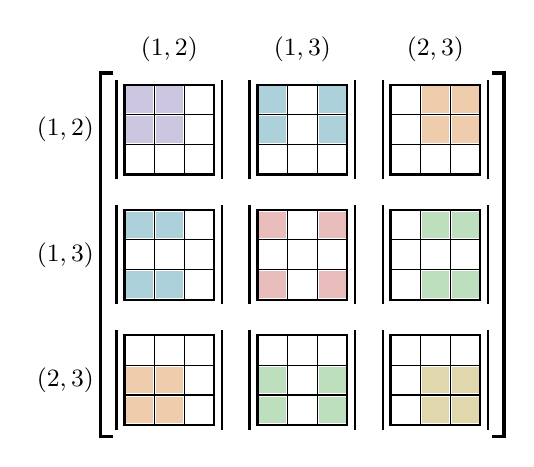
\begin{tikzpicture}[
    cell/.style={minimum size=0.38cm, inner sep=0pt},
    gridbox/.style={draw=black, thick, inner sep=0pt},
]

% We define a macro for drawing one 3x3 block at position (x,y)
% with a given color and list of highlighted cells.
% #1=x, #2=y, #3=fill color, #4=list of highlighted cells (row/col 0-indexed)
\newcommand{\drawgrid}[4]{%
  \begin{scope}[shift={(#1,#2)}]
    % Draw the grid background
    \draw[thick] (0,0) rectangle (3*0.38, 3*0.38);

    % Draw internal lines
    \foreach \i in {1,2} {
      \draw ({\i*0.38},0) -- ({\i*0.38},{3*0.38});
      \draw (0,{\i*0.38}) -- ({3*0.38},{\i*0.38});
    }

    % Fill highlighted cells
    \foreach \r/\c in {#4} {
      \fill[#3] ({\c*0.38+0.02},{(2-\r)*0.38+0.02}) 
        rectangle ({\c*0.38+0.36},{(2-\r)*0.38+0.36});
    }

    % Determinant bars
    \draw[thick] (-0.1, -0.06) -- (-0.1, {3*0.38+0.06});
    \draw[thick] ({3*0.38+0.1}, -0.06) -- ({3*0.38+0.1}, {3*0.38+0.06});
  \end{scope}
}

% ---- Define block size and spacing ----
\def\bs{1.14}    % block size = 3 * 0.38
\def\gapx{0.55}  % horizontal gap between blocks
\def\gapy{0.45}  % vertical gap between block rows

% Compute positions for the 3x3 grid of blocks
\pgfmathsetmacro{\colA}{0}
\pgfmathsetmacro{\colB}{\bs + \gapx}
\pgfmathsetmacro{\colC}{2*\bs + 2*\gapx}

\pgfmathsetmacro{\rowA}{2*\bs + 2*\gapy}
\pgfmathsetmacro{\rowB}{\bs + \gapy}
\pgfmathsetmacro{\rowC}{0}

% ---- Color definitions ----
\definecolor{colD1}{HTML}{9B8EC4}
\definecolor{colD2}{HTML}{D47B7B}
\definecolor{colD3}{HTML}{C4B05A}

\definecolor{colAB}{HTML}{5BA3B5}
\definecolor{colAC}{HTML}{E09B5A}
\definecolor{colBC}{HTML}{7BBF7B}

% ---- Draw all 9 blocks ----
\drawgrid{\colA}{\rowA}{colD1!50}{0/0, 0/1, 1/0, 1/1}

\drawgrid{\colB}{\rowA}{colAB!50}{0/0, 0/2, 1/0, 1/2}
\drawgrid{\colA}{\rowB}{colAB!50}{0/0, 0/1, 2/0, 2/1}

\drawgrid{\colC}{\rowA}{colAC!50}{0/1, 0/2, 1/1, 1/2}
\drawgrid{\colA}{\rowC}{colAC!50}{1/0, 1/1, 2/0, 2/1}

\drawgrid{\colB}{\rowB}{colD2!50}{0/0, 0/2, 2/0, 2/2}

\drawgrid{\colC}{\rowB}{colBC!50}{0/1, 0/2, 2/1, 2/2}
\drawgrid{\colB}{\rowC}{colBC!50}{1/0, 1/2, 2/0, 2/2}

\drawgrid{\colC}{\rowC}{colD3!50}{1/1, 1/2, 2/1, 2/2}

% ---- Large brackets ----
\pgfmathsetmacro{\matH}{3*\bs + 2*\gapy}
\pgfmathsetmacro{\matW}{3*\bs + 2*\gapx}
\pgfmathsetmacro{\bracketPad}{0.15}

% Left bracket
\draw[very thick] ({-\bracketPad}, {-\bracketPad}) 
  -- ({-\bracketPad - 0.15}, {-\bracketPad})
  -- ({-\bracketPad - 0.15}, {\matH + \bracketPad})
  -- ({-\bracketPad}, {\matH + \bracketPad});

% Right bracket
\draw[very thick] ({\matW + \bracketPad}, {-\bracketPad}) 
  -- ({\matW + \bracketPad + 0.15}, {-\bracketPad})
  -- ({\matW + \bracketPad + 0.15}, {\matH + \bracketPad})
  -- ({\matW + \bracketPad}, {\matH + \bracketPad});

% ---- Column labels (top) ----
\pgfmathsetmacro{\labelY}{\matH + 0.45}
\node[font=\small] at ({\colA + \bs/2}, \labelY) {$(1,2)$};
\node[font=\small] at ({\colB + \bs/2}, \labelY) {$(1,3)$};
\node[font=\small] at ({\colC + \bs/2}, \labelY) {$(2,3)$};

% ---- Row labels (left) ----
\pgfmathsetmacro{\labelX}{-0.75}
\node[font=\small] at (\labelX, {\rowA + \bs/2}) {$(1,2)$};
\node[font=\small] at (\labelX, {\rowB + \bs/2}) {$(1,3)$};
\node[font=\small] at (\labelX, {\rowC + \bs/2}) {$(2,3)$};

\end{tikzpicture}
    }
    \caption{\centering The second Gram field $G^{(2)}_M$ is constructed as a compound matrix of the first $G_M$.}
    \label{fig:compound-matrices}
\end{wrapfigure}

\paragraph{Gram fields} The \textit{$k$-th Gram field} is the mapping
\begin{equation}
    p \in M \, \, \mapsto \, \, G_M^{(k)}(p) := \Big[ \, \left\langle \iota^* dx^I,\iota^* dx^J \right\rangle_{M}(p) \, \Big]_{IJ} 
\end{equation} that assembles the collection of alignment fields into a parametrized symmetric matrix. As observed in \cite{jones2026manifolddiffusiongeometrycurvature, kawasaki2026diffusion}, the Gram field in dimension 1 is the matrix form of the projection operator
\begin{equation} 
    \Pi_p =G_M(p) : \R^D \to T_pM \subset \R^D
\end{equation} and thus recovers the tangent and normal spaces
\begin{equation}\label{eq:gramfield-decomposition}
    T_p M = \text{Im} \,G_M(p) \qquad  N_pM = \text{Ker} \, G_M(p)
\end{equation} as the respective image and kernel. As an object, the Gram field thus faithfully encodes the tangency and normal information of a submanifold as a family of $(D \times D)$-matrices parametrized by $p \in M$. Analogous decompositions hold for the $k$-th cotangent spaces (See App. \ref{app:background-diff-forms}, \ref{eq:k-normal-tangent-decomp}).


\paragraph{Inner products of forms} Define the local inner product on $k$-forms $\omega = f_I \cdot dx^I$ and $\eta = h_J \cdot dx^J$ by the mapping (using Einstein notation)
\begin{equation}
    p \, \, \mapsto \, \,  \Big(\, f^T G_M^{(k)} h\, \Big)(p) =  f_I(p) h_J(p)\left\langle \iota^* dx^I,\iota^* dx^J \right\rangle_{M}(p) 
\label{eqn:main-local-inner-product}
\end{equation} where $f$ and $h$ are the scaling vectors corresponding to $\omega$ and $\eta$ respectively. From this perspective, we interpret $G_M$ as a parametrized bilinear form on the scaling functions that preserves the tangential part and discards the normal part according to the decomposition in Equation \ref{eq:k-normal-tangent-decomp}. For a given measure $\mu$ on $M$, the \textit{global inner product} is given by
\begin{equation}
    \langle\!\langle \iota^* \omega, \iota^* \eta \rangle\!\rangle_M := \int_M \Big(f^T G_M^{(k)}h\Big)(p) d\mu,
\end{equation} i.e., the average local inner product with respect to $\mu$. Intuitively, the inner product scores the average alignment of submanifolds with pairs of ambient forms (Fig. 1).
% \begin{comment}
% \begin{intuitionbox}
%     The global inner product $ \langle\!\langle \iota^* \omega, \iota^* \eta \rangle\!\rangle_M$ is a sum of $L_2$ correlations between scaling function $$\int_M f_I(p) h_J(p)\left\langle \iota^* dx^I,\iota^* dx^J \right\rangle_{M}(p) d\mu$$ weighted by $\lrangle \iota^* dx^I,\iota^* dx^J \rangle_{M}$ . In particular, the diagonal entries measure the correlation 
%         \begin{equation}
%             \lvert f_I \rvert^2 \sim \lVert \iota^* dx^I \rVert^2_M 
%         \end{equation} between the magnitude of $I$ and the function $\lVert \iota^* dx^I \rVert^2_M$ describing the volume of the $k$-cube in $I$ projected onto $M$. {\color{red}K: is this even helpful LOL }
% \end{intuitionbox}
% \end{comment}

\begin{comment}
\section{Background Old}



Let $V$ be an inner product space with inner product $\langle-, -\rangle$. The \textit{Gram matrix} of a tuple $(v_1, \ldots, v_\ell)$ of vectors $v_i \in V$ is the matrix
\begin{equation}
    G(\mathbf{v}) = \Big[ \langle v_i,v_j \rangle \Big]_{i,j} \in \R^{\ell \times \ell}.
\end{equation}

\paragraph{Riemannian metrics} A Riemannian metric $g$ on a manifold $M$ corresponds to a family of inner products
\begin{equation}
    \langle -, - \rangle_g : T_p M \otimes T_pM \to \R
\end{equation} parametrized by points $p \in M$. Let $\Delta_g : C^\infty(M) \to C^\infty(M)$ be the Laplace-Beltrami operator on smooth functions. The \textit{Carré-du-champ} identity
\begin{equation}
    \big\langle \,df, dh \,\big\rangle_{g_M}(p) = \Gamma_{\Delta_g}(f,h) :=\dfrac{1}{2} \Big( f \Delta_g h + h \Delta_g f - \Delta_g(fh) \Big)(p)
\end{equation} relates the inner product on the differentials $df,dh \in \Omega^1(M)$ of smooth functions $f,h \in C^\infty(M)$ with the Laplace-Beltrami operator and the point-wise multiplication of functions. 


\paragraph{Differential forms} A formal and unhelpful definition of a \textit{differential $k$-form} $\omega \in \Omega^k(M)$ on a manifold $M$ is as a smooth section of the $k$-th exterior algebra of the cotangent bundle (See \ref{app:recollections}). Equivalently, $\omega \in \Omega^k(M)$ specifies a family of alternating functions
\begin{equation}
    \omega_p : T_pM \times \ldots \times T_pM \to \R
\end{equation} parametrized over points $p \in M$. This function $\omega_p$ takes as input $(k+1)$ \todo[P: why $k+1$ and not $k$?]{} tangent vectors $(v_0, \ldots, v_k)$ at $p$ and outputs a real number, loosely interpreted as volume spanned by $(v_0, \ldots, v_k)$ with respect to $\omega$.

\paragraph{Ambient forms} In Euclidean space, differential $k$-forms exhibit a convenient global structure. Explicitly, for coordinate functions $(x_1, \ldots, x_D)$ on $\R^D$, the differential $k$-forms in $\R^D$ satisfy the following isomorphism
\begin{equation}
    \Omega^k(\R^D) \cong C^\infty(M) \otimes \Lambda^k(dx_1, \ldots, dx_D)
\end{equation} \todo[V: $C^\infty(\mathbb R^D)$ I think] where the tensor product is over $\R$ and $\Lambda^k(dx_1, \ldots, dx_D)$ is the $k$-th exterior algebra over the symbols $dx_1, \ldots, dx_D$. In other words, this means that every differential $k$-form in $\R^D$ can be written in a canonical form\footnote{Employing Einstein notation.}
\begin{equation}
    \omega = f_I \cdot dx_I := \sum_I f_I \cdot dx_I
\end{equation} for some smooth \textit{scaling function} $f_I \in C^\infty(\R^D)$ and basis form $dx_I \in \Lambda^k(dx_1, \ldots, dx_D)$, where $I$ ranges over multi-indices $I = (1\leq i_1 < \cdots < i_k \leq D)$.
\end{comment}
\begin{comment}
\begin{intuitionbox}
Let $I = (1\leq i_1 < \cdots < i_k \leq D)$ be a multi-index. For a tangent vector $v \in T_p \R^D$, let $v^I$ denote the projection of $v$ under $T_p \R^D \to T_p\R^I$.
\begin{enumerate} 
    \item (Basis forms) For each $p \in \R^D$, the basis form $$dx^I = dx^{i_1} \wedge \ldots \wedge dx^{i_k}$$ corresponds to the alternating function
    \begin{equation}
        dx^I_p : T_p\R^D \times \ldots \times T_p\R^D \to \R; \hspace{3em} dx_p^I(v_1, \ldots, v_k) = \det_{s,r} \big[v_s^I, v_r^I \big],
    \end{equation} i.e., the Euclidean volume spanned by the tangent vectors in the $I$-subspace.
    \item (Scaling functions) The function $$f_I : \R^D \to \R$$ \textit{rescales} the volume in the $I$-subspace at $p$ by $f_I(p)$. A negative sign implies a reversal of orientation.
\end{enumerate}
\end{intuitionbox}
\end{comment} 
\begin{comment}
\paragraph{Pullbacks} Suppose we have a smoothly embedded manifold $\iota : M \hookrightarrow \R^D.$ Since $\iota$ is an embedding, there are natural inclusions and orthogonal projections of tangent spaces
\begin{equation}
    T_p M \hookrightarrow T_p \R^D \xrightarrow{\Pi_x} T_p M
\end{equation} at each point $p \in M$. Let $\omega \in \Omega^k(\R^D)$. The \textit{pullback form} $\iota^*\omega \in \Omega^k(M)$ of $\omega$ along $\iota$ is the differential $k$-form defined by the family of alternating functions
\begin{equation}
    \iota^*\omega_p : T_pM \times \ldots \times T_pM \to \R; \hspace{2em} \iota^*\omega_p(v_1, \ldots, v_k) = \omega_{\iota(p)}(v_1, \ldots, v_k)
\end{equation} where we have identified $v_p \in T_pM$ with its inclusion into $T_p\R^D$.

\begin{remark} Pullbacks of differential forms onto a submanifold detect meaningful tangency information. For example, any embedded submanifold $\iota : M \hookrightarrow \R^D$ satisfies
\begin{equation}
    T_pM \perp T_p \R^I \Rightarrow \iota^* dx^I_p = 0 \hspace{2em} \text{and} \hspace{2em} T_pM \subset T_p\R^I \Rightarrow \iota^* dx_p^I = dx_p^I
\end{equation} for any multi-index $I$. \end{remark}



\paragraph{Point-wise inner products} For a point $p$, the metric $g$ induces a family of inner products on the cotangent space
\begin{equation}
    \langle -, -\rangle_g : T_p^*M \otimes T_p^*M \to \R
\end{equation} For embedded submanifolds $\iota : M \hookrightarrow \R^D$ with induced metrics with orthogonal projections $\Pi_p : T_p \R^D \to T_p M$ onto the tangent space. Let $\partial_{x_i}(p) \in T_p\R^D$ be the tangent vector in direction $x^i$ at $p$. The inner product on basis $1$-forms satisfies
\begin{equation}
    \Big\langle \iota ^*dx^i_p, \iota^*dx^j_p \Big\rangle_g = \Big\langle \Pi_p \partial_{x_i}, \Pi_p \partial_{x_j} \Big\rangle_{\R^D}(p)
\end{equation} and, by linearity,
\begin{equation} \label{eq:innerprod-1forms}
    \Big\langle \iota^* f^idx^i_p, \iota^*h^jdx^j_p \Big\rangle_g =  f^i(p)h^j(p)\Big\langle \iota^* dx^i, \iota^* dx^j \Big\rangle_{g}(p) = f^i(p)h^j(p)\Big\langle \Pi_p \partial_{x_i}, \Pi_p \partial_{x_j} \Big\rangle_{\R^D}(p).
\end{equation} 

\begin{intuitionbox}
    The local inner product of two $1$-forms $\iota^* f^idx^i_p$ and $\iota^*h^jdx^j_p$ \todo[P: at $p$]{} is 
    \begin{enumerate}
        \item positive when scaling functions agree on tangential directions to $M$.
        \item negative when scaling functions disagree on tangential directions to $M$.
        \item zero in normal directions to $M$.
    \end{enumerate}
    \todo[P: What does "disagreeing on tangential directions" mean when we compare forms living in the same space? Is negativity/positivity more related to agreement in orientation?]{}
\end{intuitionbox}



Higher-order local inner products are defined by extending the
one-form pairing to exterior powers. For multi-indices
$I=(i_1<\cdots<i_k)$ and $J=(j_1<\cdots<j_k)$, set
\begin{equation}
\left\langle \iota^* dx^I,\iota^* dx^J \right\rangle_{g_M}(p)
:=
\det\left[
\left\langle
\iota^* dx^{i_a},
\iota^* dx^{j_b}
\right\rangle_{g_M}(p)
\right]_{a,b=1}^k .
\end{equation}
This extends to ambient $k$-forms $\omega = f_I dx^I$ and $\eta = h_J dx^J$ in $\Omega^k(\R^D)$ then
\begin{equation}
\left\langle \iota^*\omega,\iota^*\eta \right\rangle_{g_M}(p)
=
f_I(p)h_J(p)
\left\langle
\iota^* dx^I,\iota^* dx^J
\right\rangle_{g_M}(p)
\end{equation}



\paragraph{$L^2$ inner products}
The pointwise pairing of $k$-forms defines a real-valued function on $M$.
For $\alpha,\beta \in \Omega^k(M)$, we write this function as
\begin{equation}
p \longmapsto \langle \alpha,\beta\rangle_{g_M}(p).
\end{equation}
A global comparison is obtained by integrating this pointwise pairing over
the manifold. Given a measure $\mu$ on $M$, define
\begin{equation}
\left\langle\!\left\langle
\alpha,\beta
\right\rangle\!\right\rangle_{L^2(M,\mu)}
:=
\int_M
\left\langle
\alpha,\beta
\right\rangle_{g_M}(p)
\,d\mu(p).
\end{equation}
In the unweighted case, $\mu=dV_{g_M}$ is the Riemannian volume measure. If
$q:M\to\mathbb{R}_{\geq 0}$ is a sampling density \todo[P: at this point no notion of sampling introduced]{}, we may instead take
$\mu=q\,dV_{g_M}$. Since our forms arise by restricting ambient forms to $M$, for
$\omega,\eta\in\Omega^k(\mathbb{R}^D)$ we define
\begin{equation}
\left\langle\!\left\langle
\iota^*\omega,\iota^*\eta
\right\rangle\!\right\rangle_{L^2(M,\mu)}
=
\int_M
\left\langle
\iota^*\omega,\iota^*\eta
\right\rangle_{g_M}(p)
\,d\mu(p).
\end{equation}
This global inner product measures how similarly the ambient forms
$\omega$ and $\eta$ are activated \textit{on average} along the tangent geometry of $M$.
\end{comment}


\section{Neural Point-Forms}
\label{sec:formulation}
% Drawing heavily from ideas in \cite{jones2024manifold} and \cite{jones2026computing}, the central object from extrinsic manifold theory we approximate is the pullback matrix
% \begin{equation} 
% \langle \iota^* dx^I, \iota^*dx^J\rangle_{g_M}(p)
% \end{equation} of inner products of ambient basis forms. The key observation is that such quantities can estimated via the $0$-Laplacian (which has a well-established estimation theory) using the Carré-du-champ relation. 

%avoiding jumping too harshly from "laplacians have theory" to "our pairings are estimated" 

We now translate the theory above into the point cloud setting using the techniques of Diffusion Geometry \cite{jones2026manifolddiffusiongeometrycurvature, jonesComputingDiffusionGeometry2026}. We show our estimators are consistent, and detail how our constructions lead naturally to a algorithms for processing point clouds.

%Rather than approximating the manifold structure directly, the perspective introduced inin to use the Gram field as a manifold-like representation that is computable in practice. The key observation is that, under the smooth-manifold sampling assumptions used in Appendix~\ref{appendix:B}, the carré du champ identity lets us estimate the required contangent pairings from a graph operator that approximates the continuum diffusion generator. %\todo[P: I think we should point out here that we don't know the manifold or the map $\iota$ but want to learn it from the implied inner product that is related to laplace operator which can be approximated in a discrete setting.]{}

%Our main contributions are to show how this (1) combines with a theory of learnable differentiable form-based representations of space and (2) to work through the details of consistency results and their specific convergence properties. 


\begin{comment}
\paragraph{Gram fields of sub-manifolds}  Re-formalizing this for our setting, define the \textit{extrinsic Gram field} of an embedded submanifold $\iota : M \hookrightarrow \R^D$ as the function
\begin{equation}
    p \in M \mapsto G_M(p) = \Big[ \langle \iota^* dx^i, \iota^* dx^j \rangle_M(p)\Big] \in \text{Sym}\,\R^{D \times D}.
\end{equation} The inner product of pullbacks of $1$-forms $f^idx^i, h^j dx^j \in \Omega^1(\R^D)$  in \ref{eq:innerprod-1forms} can be written in matrix notation as
\begin{equation} 
     \Big\langle \iota^* f^idx^i, \iota^*h^jdx^j \Big\rangle_g(p) = \begin{bmatrix} f^1(p) & \cdots & f^D(p) \end{bmatrix} G_M(p) \begin{bmatrix} h^1(p) \\ \vdots \\ h^D(p) \end{bmatrix}
\end{equation} Analogously, the \textit{$k$-th extrinisc Gram field} is the mapping
\begin{equation}
    p \in M \mapsto G^{(k)}_M(p) :=  \Big[ \langle \iota^*dx_I, \iota^*dx_J\rangle_g(p) \Big]_{IJ} = \Big[ \det G^{IJ}_M(p) \Big]_{IJ} = \Bigg[  \det_{s, r \in [k]}[G^{i_{s}j_{r}}] \Bigg]_{IJ} \in \R^{\binom{D}{k} \times \binom{D}{k}}.
\end{equation} where $I$ and $J$ range over multi-indices
\begin{equation}
    I = (i_1 < \ldots < i_k) \hspace{2em} \text{and} \hspace{2em} J = (j_1 < \ldots < j_k).
\end{equation} As above, the inner product of pullbacks of $k$-forms $f_Idx^I, h_J dx^J \in \Omega^k(\R^D)$  in \ref{eq:innerprod-1forms} can be written in matrix notation as
\begin{equation} 
     \Big\langle \iota^* f_Idx^I, \iota^*h_Jdx^J \Big\rangle_{g_M}(p) = \begin{bmatrix} f^{I}(p) & \cdots & \end{bmatrix} G_M(p) \begin{bmatrix} h^J(p) \\ \vdots \\ 
     \end{bmatrix}
\end{equation}



\paragraph{Ambient Gram matrices of manifolds} Following \cite{jones2026manifolddiffusiongeometrycurvature}, the first quantity we approximate at a point $p \in M$ is the symmetric Gram matrix
\begin{equation}
    G_{M}(p)  := \Big[ \langle \iota^*dx_i, \iota^*dx_j\rangle_g(p) \Big] \in \R^{D \times D,} 
\end{equation} of pullback of pairs of ambient coordinate functions. Equivalently, this specifies a symmetric bilinear operator
\begin{equation}
    G_{M}(p) : T_p^* \R^D \otimes T_p^* \R^D  \to \R;\hspace{2em} (v,w) \mapsto v^T \, G_M \, w
\end{equation} on the cotangent space at $p$ where $v$ and $w$ are row vectors in the standard basis. A basic result (noted in \cite{Jones2024DiffGeom}) to highlight is the following.
\begin{proposition}
    Let $\iota : M \hookrightarrow \R^D$ be the inclusion of an embedded sub-manifold with induced metric $g$. For all $p \in M$ and $v,w \in T_p^*\R^D$
    \begin{equation}
        G_M(p)(v,w)= \langle \iota^*v,\iota^*w\rangle_g.
    \end{equation}
\end{proposition} Conceptually, approximating $G_M(p)$ permits approximation of the inner product on the cotangent space without access to the underlying manifold structure.

\begin{remark} To build intuition, consider the following consequence of the above -- if $N_p^* M$ is the normal cotangent space at $p$, this immediately implies that
\begin{equation}
    (v,v) \in \ker G_M(p) \Leftrightarrow v\in N_p M. 
\end{equation} 
\end{remark}

The same reasoning works perfectly well for the $k$-th cotangent space. At a point $p$, the \textit{$k$-th ambient gram matrix} is 
\begin{equation}
    G^{(k)}_M(p) :=  \Big[ \langle \iota^*dx_I, \iota^*dx_J\rangle_g(p) \Big]_{IJ} = \Big[ \det G^{IJ}_M(p) \Big]_{IJ} = \Bigg[  \det_{s, r \in [k]}[G^{i_{s}j_{r}}] \Bigg]_{IJ} \in \R^{\binom{D}{k} \times \binom{D}{k}}.
\end{equation} where $I$ and $J$ range over multi-indices
\begin{equation}
    I = (i_1 < \ldots < i_k) \hspace{2em} \text{and} \hspace{2em} J = (j_1 < \ldots < j_k).
\end{equation} Considering $G_M^{(k)}$ as an $M$-parametrized family of bilinear operators
\begin{equation}
    G_M^{(k)}(p) : \Lambda^k T_p^* \R^D \otimes \Lambda^kT_p^* \R^D  \to \R
\end{equation} on the $k$-th exterior power of the cotangent space at $p$, the following proposition holds by analogous arguments for the $1$-dimensional case. 

\begin{proposition}
    Let $\iota : M \hookrightarrow \R^D$ be the inclusion of an embedded sub-manifold with induced metric $g$. For all $p \in M$ and $v,w \in \Lambda^kT_p^*\R^D$
    \begin{equation}
        G_M^{(k)}(p)(v,w)= \langle \iota^*v,\iota^*w\rangle_g.
    \end{equation}
\end{proposition} 
\end{comment}

\paragraph{Discrete \CdC.}
Suppose now that $P \subset \mathbb{R}^D$ is a finite point cloud. Since $P$
is discrete, it does not have a nontrivial tangent or cotangent bundle. We
therefore replace the smooth Laplace--Beltrami operator by a discrete
Laplacian $L_P : \mathbb{R}^P \to \mathbb{R}^P$ where $\mathbb{R}^P$ is the set of functions $f: P \to \R$. In our implementation, $L_P$ is taken to be the discrete variable-bandwidth Laplacian, since it is well-equipped for dealing with noisy nonuniform samples in practice~\ref{discrete-variable-bandwidth-laplacian} from \cite{Berry2016}. The corresponding \textit{discrete \cdc} is the bilinear map
\begin{equation}
\Gamma_{L_P}(f,h)(p)
:=
\frac{1}{2}
\Big(
f(p)L_P h(p)
+
h(p)L_P f(p)
-
L_P(fh)(p)
\Big),
\qquad
f,h \in \mathbb{R}^P,\ p\in P,
\end{equation}
where $fh$ denotes pointwise multiplication.

\paragraph{Gram fields on point clouds} Let $x^i : P \to \mathbb{R}$ denote the restriction of the $i$th ambient
coordinate function to $P$. For $k\geq 1$, the $k$th extrinsic Gram field is the map $
G_P^{(k)} : P \to \R^{\binom{D}{k}\times \binom{D}{k}}$
whose entries are indexed by increasing multi-indices
$I=(i_1<\cdots<i_k)$ and $J=(j_1<\cdots<j_k)$ and are given by
\begin{equation}
\left(G_P^{(k)}(p)\right)^{IJ}
:=
\det
\left[
G_P^{i_a j_b}(p)
\right]_{a,b=1}^k
=
\det
\left[
\Gamma_{L_P}(x^{i_a},x^{j_b})(p)
\right]_{a,b=1}^k .
\end{equation}
Intutively, the discrete \cdc \textit{defines} the discrete alignment field, motivated by equality witnessed via the smooth \cdc formula \ref{smooth-carre-du-champ}. We thus think of $G_P^{(k)}(p)$ as the discrete analogue the smooth Gram field.

\begin{comment}
\paragraph{Comparison matrices} Now suppose we have a family of ambient differential forms $\mathbf{\omega} = (\omega^{(1)}, \ldots, \omega^{(\ell)})$ in $\Omega^k(\R^D)$. The \textit{comparison matrix} of a sub-manifold $\iota : M \hookrightarrow \R^D$ against $\mathbf{\omega}$ is
\begin{equation}
    \Big[ \big\langle \iota^* \omega^{(i)}, \iota^* \omega^{(j)}\big\rangle_{g_M} \Big] \in \R^{\ell \times \ell}.
\end{equation} The comparison matrix provides a mapping:
\begin{equation}
   \Big\{  \, \text{Embedded sub-manifolds: } \, \iota : M \hookrightarrow \R^D \,\Big\} \mapsto \Big\{ \, \text{Symmetric matrices:} \, \, \text{Sym} \, \R^{\ell \times \ell}  \, \Big\}
\end{equation} which we employ as a vectorization scheme for embedded manifold data in a shared ambient space. 

From this perspective, the differential forms $\omega^{(i)}$ are higher-order features on the ambient space $\R^D$. The data of a comparison matrix contain the information how ambient feature forms are activated and cross-activated by the tangency information of the manifold. 
\end{comment}

\paragraph{Discrete inner products of forms} Inner products on forms over a point cloud are defined analogously to smooth case, i.e., via the discrete Gram field as a parametrized bilinear operator. Explicitly,  $\omega = f_I \cdot dx^I$ and $\eta = h_J \cdot dx^J$ define the local inner product on $k$-forms over $P$ by the mapping
\begin{equation} \label{def:gramfield-innerproduct}
    p \, \, \mapsto \, \,  \big\langle \, \omega, \eta \, \big\rangle_P(p) := \Big(\, f^T G_P^{(k)} h\, \Big)(p).
\end{equation} Similarly, for a discrete measure $\mu_P$ on $P$, define the global inner product of $\omega$ and $\eta$ by
\begin{equation}
\label{def:gramfield-global-inner-product}
    \llangle \omega, \eta \rrangle_P = \sum_{p \in P} \langle \, \omega, \eta \, \rangle_P(p) \mu(p).
\end{equation}


\paragraph{Consistency results} We formalize the claim 

%suggestive notation\jake{notation or notion?}\kelly{notation} \jake{like viewing all of (19) as a piece of notation? haha} that
\begin{equation}
    \llangle \omega ,\eta \rrangle_P \qquad \text{is an estimator of} \qquad \llangle \iota^*\omega, \iota^*\eta\rrangle_M
\end{equation} when $P \subset \R^D$ is sampled from an embedded submanifold $\iota : M \hookrightarrow \R^D$. Appendix~\ref{appendix:B} contains a detailed discussion, from which we extract the following. 

\begin{informalthm}{Continuum Limits}{main-text-continuum-limits}
%\label{thm:main-text-continuum-limits}
% $q$, from which a point cloud $P=\{ p_{i} \overset{\text{i.i.d.}}{\sim} q \}_{i=1}^n$
    Let $M \subset_{\iota} \R^D$ be a manifold with probability density \( q \) from which point clouds $P_{n}=\{ p_{i} \overset{\text{i.i.d.}}{\sim} q \}_{i=1}^n$ are sampled. For each $P_n$, construct the local inner product \( \langle -,-  \rangle_{P_{n}}  \)~\ref{def:gramfield-innerproduct} using the variable-bandwidth Laplacian \( L_{P} \) as described in Appendix~\ref{appendix:B}.  Let $\omega, \eta \in \Omega^k(\mathbb{R}^{D})$. %Then:
  
    \begin{enumerate}
        \item \textit{(Local)}  For any $p \in M$,
    \begin{equation}
        \lim_{n \to \infty} \langle\, \omega, \eta \, \rangle_{P_n}(p) = \langle \iota^*\omega, \iota^*\eta\rangle_M(p) \text{ almost surely},
        \label{eqn:main-text-local-continuum}
    \end{equation} and this convergence is uniform in \( p \) provided \( M \) is compact.
        \item \textit{(Global)} If \( M \) is compact, then
    \begin{equation}
        \lim_{n \to \infty} \llangle\, \omega, \eta \, \rrangle_{P_n} = \llangle \iota^*\omega, \iota^*\eta\rrangle_M \text{ almost surely},
        \label{eqn:main-text-global-continuum}
    \end{equation} where the summation~\eqref{def:gramfield-global-inner-product} is against a standard choice of \( \mu \in \mathbb{R}^{P} \).
    
    %\todo[sampling-aware inner product-y stuff maybe]
    \end{enumerate}
   
\end{informalthm} 

\begin{proof}[Proof (Sketch)]
    


In order to prove Theorem~\ref{ithm:main-text-continuum-limits}, we first provide an expansion on the observation in~\cite{jones2026manifolddiffusiongeometrycurvature}, itself based on \cite{Berry2016}, that the discrete Gram field $G^{(1)}_{P}$ consistently estimates the continuous Gram field $G^{(1)}$. Specifically, we
\begin{enumerate}
    \item analyze how the variable-bandwidth Laplacian parameters affect convergence rates in low-sampling density regions likely to occur in practice (Corollary~\ref{cor:cdc-consistency});
    \item explicate exponential probability bounds under which consistency holds uniformly in the \( (i,j) \)-alignment fields comprising \( G^{(1)} \)(Lemma~\ref{lemma:uniformizing-in-f}); and
    \item explicate exponential probability bounds under which consistency holds uniformly in $p$ when $M$ is compact (Lemma \ref{lemma:uniformizing-in-i-with-compactness}). 
\end{enumerate}
These additional pieces allow us to push consistency estimates on $G^{(1)}$ (Proposition~\ref{prop:tangential-projector-consistency}) uniformly through the determinantal structure~\eqref{eqn:IJ-alignment-field}  in the \( (I,J) \)-alignment fields defining $G^{(k)}$ (Proposition~\ref{cor:kth-tangential-projector-consistency} and Corollary~\ref{cor:kth-tangential-projector-compactness-corollary}), and in turn the local inner product~\eqref{eqn:main-local-inner-product} (Theorem \ref{thm:locla-consistency-estimate}), from which we are able to extract the local continuum limit \eqref{eqn:main-text-local-continuum} almost surely by way of the probability bounds' exponentiality (Corollary~\ref{cor:local-continuum-limit}). Using $(3)$, we further deduce this convergence to be uniform in $p$ when $M$ is compact, and this underlies our further extraction of the global continuum limit~\eqref{eqn:main-text-global-continuum} (Corollary~\ref{cor:global-continuum-limit}). 
\end{proof}
 A feature of our theory is its faithfulness to practice. Our results hold, up to $k$-NN truncation, for the flexible class of variable-bandwidth Laplacians $\Delta_{P}$ used in our implementation. Moreover, they include explicit finite-sample dependence upon (and provable insensitivity to) estimation parameters for $\Delta_{P}$. All of our results also accommodate nonuniform sampling; in the local case \textit{arbitrarily} nonuniform from an unknown density. %\kelly{great} 

\begin{comment}

\begin{informalthm}{Local inner product convergence}{prop:local-inner-prod-convergence}
    Let $\iota : M \hookrightarrow \R^D$ be an embedded manifold, $q$ be a density of $M$ and $P_n = \{ p_1, \ldots, p_n \} \subset M$ be a set of $n$ points sampled i.i.d. with $p_i \sim q$. For each $P_n$, construct the discrete Gram field and inner product using the variable bandwidth Laplacian described in \ref{appendix:B}. Then for any $p \in M$ and $\omega, \eta \in \Omega^k(M)$, we have
    \begin{equation}
        \lim_{n \to \infty} \langle\, \omega, \eta \, \rangle_{P_n}(p) = \langle \iota^*\omega, \iota^*\eta\rangle_M(p)
    \end{equation} almost surely. and this convergence is uniform in \( p \) provided \( M \) is compact.
\end{informalthm} We note that result follows quickly from the observation in \cite{jones2026manifolddiffusiongeometrycurvature} that the discrete Gram field is an estimator of the continuous Gram field. We expand on the proof given there by analyzing how the parameters of the variable bandwidth Laplacian affect convergence rates in low-sampling density regions likely to occur in practice. The global statement is as follows. \jake{(from J to J: we can't and don't actually build on Iolo directly because of subtleties regarding uniformity, find a way to credit Iolo 3.2 without implying that we are a direct corollary of it)}

\begin{informalthm}{Global inner product convergence}{prop:global-inner-prod-convergence} Let $M, P_n, q$ and the inner product be defined as in Prop. \ref{prop:local-inner-prod-convergence}.  For each $P_n$, construct the discrete Gram field and inner product using the variable bandwidth Laplacian described in \ref{appendix:B}. Then for any $\omega, \eta \in \Omega^k(M)$, we have
    \begin{equation}
        \lim_{n \to \infty} \llangle\, \omega, \eta \, \rrangle_{P_n} = \llangle \iota^*\omega, \iota^*\eta\rrangle_M
    \end{equation} almost surely. \kelly{Add in two density correction cases? Also, which point cloud inner product notation are we using -- do you still prefer the pullback $\llangle P^* \omega, P^*\eta \rrangle?$} \jake{I personally prefer the `formal/implicit restriction/pullback' notation \( P^{*} \) (and likewise \( M^{*} \) in smooth setting, distinct from the earnest pullback/restriction \( \iota ^*\)) notation throughout to make it clear that we are never defining differential forms intrinsically on point clouds, only accessing them implicitly by way of formal restriction + pairing (and this is why we can get away with a large simplification of Iolo's definition)}
\end{informalthm}


{\color{red} TO DO: PUT INFORMAL VERSIONS OF CONSISTENCY THEOREMS}
\todo[J: maybe a sentence to although we choose to elide statement of assumptions underlying our theory here, these assumptions are in fact quite relaxed.. just something like 'up to X, our theory holds for the exact thing we implement (specifically we have flexible assumptions regarding sampling density (and knowledge of it), compactness, kernel construction (bandiwdith, hyperparams) ]

\todo[still need to update notation below (]
\begin{corollary}[Local Continuum - Informal]
    For any $p_{i} \in P$, $$\lim_{n \to \infty} \langle P^{*}\omega, P^{*} \eta \rangle_{P} (p_{i})=\langle \iota^{*}\omega, \iota^{*}\eta \rangle_{g}(p_{i})$$
almost surely, and this convergence may be taken uniform in $p_{i}$ provided $M$ is compact. 
\end{corollary}
\todo[P: introduce new symbols $n, \iota$. J: these will be standardized once decide \( \iota  \)vs \( \iota \) (plspls \( \iota \)). the \( g \) subscript maybe changes by now, did we decide on \( _{M}  \) or?] {\color{red} K: yes we will definitely change to iota}
\begin{corollary}[Global Continuum - Informal]
    If \( M \) is compact, then $$\lim_{n \to \infty} \langle \! \langle P^{*}\omega, P^{*}\eta \rangle  \! \rangle _{L^2(P,  \mu_{P})}=\langle \! \langle \iota^{*}\omega, \iota^{*}\eta \rangle \! \rangle_{L^2(M, \mu)} $$almost surely.
\end{corollary}


\begin{remark}[Contribution]
    \todo[I would like to be somewhat precise about our contribution here, given this is somewhat implicit already in Iolos' paper. The global one with and without density correction is definitely new, and I think it's worth mentioning we keep track of rates and are careful about uniformity in a detailled appendix. ] \todo[J: yes: locally-- the rates, uniformity, and explicit tracking of probability bounds are what we have for the cdc estimation that Iolo corollary 3.2 doesn't, and then we are able to use this more thorough characterization of cdc consistency to extend beyond \( k=1 \). I guess Iolo also doesn't show his estimate is uniform in \( p \) even though his manifolds are compact (in part because imo to do this rigorously one should precisely interface with BH, which he - very understandably I've learned - avoids). And then yeah the global stuff is not much Iolo ]
\end{remark}

\kelly{Jake, can you write the above in paper format instead of a comment?}
\end{comment}




\paragraph{Neural $k$-forms.} The key observation is that ambient differential forms are completely characterized by their scaling functions. This means that differential forms can be parametrized as neural networks and back-propagated over learning tasks \cite{maggs2023simplicial}. Let $\Theta$ denote the parameter space, and let
\begin{equation}
F_{\theta}:\mathbb{R}^D
\to
\mathbb{R}^{\ell \times \binom{D}{k}}
\end{equation}
be a neural network with parameters $\theta \in \Theta$. For each $a\in\{1,\ldots,\ell\}$, the $a$th row of
$F_\theta$ defines the scaling functions of an ambient $k$-form
\begin{equation}
\omega_{\theta}^{(a)}
=
\sum_I
F_{\theta}^{aI} \cdot dx^I
\in \Omega^k(\mathbb{R}^D),
\end{equation}
parametrized by $\theta$. 

\paragraph{Comparison matrices} The final step is to produce an interpretable, learnable vectorization of point-cloud data that depends parametrically on a collection of ambient neural $k$-forms. Given a point cloud $P$, the neural $k$-forms produce the learnable \textit{comparison matrix}
\begin{equation}
\left(C_P(\theta)\right)_{ab} := \llangle \omega^{(a)}, \omega^{(b)} \rrangle_P = 
\sum_{p\in P}
\,
F_{\theta}^{a}(p)^\top
G_P^{(k)}(p)
F_{\theta}^{b}(p) \mu_P(p)
\end{equation}
where $F_{\theta}^{a}(p)\in\mathbb{R}^{\binom{D}{k}}$ denotes the $a$th row of
$F_\theta(p)$. The comparison matrix mapping \begin{equation}
P \, \, 
 \mapsto \, \, 
C_P(\theta)
\in \R^{\ell \times \ell}
\end{equation} represents each point cloud as an $(\ell \times \ell)$-matrix and is permutation-invariant in the points of $P$. It's dimension depends on the number of features rather the number of points. It's entries correspond to inner products of global ambient features, and are across samples in the shared ambient feature space.


\paragraph{Architecture} A key point is that the above theory leads to a straightforward and efficient architecture. Fix an ambient space $\R^D$ consisting of the global features, form dimension $k$ and choice of Laplacian for each point cloud. Intialize a neural $k$-form 
\begin{equation} 
F_\theta: \R^D \to \R^{\ell \times \binom{D}{k}}
\end{equation} with $\ell$ features. Choose a density $\mu_P$ for each point cloud $P$ in the dataset.
\begin{enumerate}
    \item (Gram field transform) The first step performs the mapping
    \begin{equation} 
\Big\{ P \subset \R^D \Big\} \hspace{2em} \mapsto \hspace{2em} \Big\{ G_P^{(k)} : P \to  \R^{\binom{D}{k} \times \binom{D}{k}} \Big\}  
\end{equation} that represents each point cloud $P$ in a dataset by it's Gram field, in practice, a tensor of size $P \times \binom{D}{k} \times \binom{D}{k}$. Since this requires the (expensive) computation of compound matrices, this is performed as pre-computation step as in Algorithm \ref{alg:gram-field}.
\item (Comparison matrix pass) The comparison matrix layer is the mapping
 \begin{equation} 
\big(\,G_P^{(k)}\, , F_\theta \, \big)  \hspace{2em} \mapsto \hspace{2em}\left(C_P(\theta)\right)_{ab} := 
\sum_{p\in P}
\,
F_{\theta}^{a}(p)^\top
G_P^{(k)}(p)
F_{\theta}^{b}(p) \mu_P(p)
\end{equation} described in Algorithm  \ref{alg:comparison-matrix}. This layer is in the forward pass -- the parameters can be thus be back-propagated against any downstream learning task. As per the right-hand side above, this simply requires summing the evaluations of neural scaling vectors against the bilinear forms $G_P^{(k)}(p)$ over $p$ for each pair $1 \leq a\leq b \leq \ell$.  
\end{enumerate} In practice, we vectorize $C_P(\theta)$ with various readout layers, for example
by taking its upper triangular entries, and pass the resulting feature vector to a downstream classifier. 


\begin{comment}
\paragraph{Gram field transformation} In the precomputation step, we first eplace each point cloud with a Gram field to represent it as an discrete, manifold-like structure as per Algorithm \ref{alg:gram-field}. Explicitly, fix an ambient feature space $\R^D$. Each pointform
\begin{equation} 
\Big\{ P \subset \R^D \Big\} \hspace{2em} \mapsto \hspace{2em} \Big\{ G_P^{(k)} : P \to  \R^{\binom{D}{k} \times \binom{D}{k}} \Big\}  
\end{equation} by replacing each point cloud $P$ in the dataset by its corresponding Gram field $G^{(k)}_P$ for some choice of $k$. Since this requires the computation of many compound matrices, this is performed as pre-computation step via the following algorithm.


\paragraph{Comparison matrix forward pass} Our contribution to the forward pass is the passage from a point cloud $P$ to the learnable comparison matrix $G_P$ of \todo[P: finish this]{}


\paragraph{Pooling and readout}

\todo[J: pooling discussion would go around here i suppose]
\end{comment}
\begin{comment}
\paragraph{Comparison matrices of submanifolds.}
Let
\[
\boldsymbol{\omega}
=
(\omega^{(1)},\ldots,\omega^{(\ell)})
\subset \Omega^k(\mathbb{R}^D)
\]
be a collection of ambient $k$-forms. Given an embedded submanifold
$\iota:M\hookrightarrow\mathbb{R}^D$ and a measure $\mu$ on $M$, we define
the comparison matrix of $M$ against $\boldsymbol{\omega}$ by
\begin{equation}
C_M^{\boldsymbol{\omega}}
:=
\left[
\left\langle\!\left\langle
\iota^*\omega^{(a)},\iota^*\omega^{(b)}
\right\rangle\!\right\rangle_{L^2(M,\mu)}
\right]_{a,b=1}^{\ell}
\in \operatorname{Sym}_{\ell}.
\end{equation}
Thus $C_M^{\boldsymbol{\omega}}$ records the pairwise global activations of
the ambient forms after restriction to the tangent geometry of $M$.

Writing
\begin{equation}
\omega^{(a)}
=
\sum_I f_I^{(a)} dx^I,
\end{equation}
where $I$ ranges over increasing $k$-multi-indices, the entries of the
comparison matrix can be expressed in terms of the extrinsic Gram field as
\begin{equation}
\left(C_M^{\boldsymbol{\omega}}\right)_{ab}
=
\int_M
f^{(a)}(p)^\top
G_M^{(k)}(p)
f^{(b)}(p)
\,d\mu(p).
\end{equation}
Here $f^{(a)}(p)=(f_I^{(a)}(p))_I$ is the coefficient vector of
$\omega^{(a)}$ at $p$, and $G_M^{(k)}(p)$ is the $k$th extrinsic Gram field.
Equivalently, the comparison matrix is a matrix-valued readout obtained by
averaging local Gram-weighted inner products of form coefficients.

\paragraph{Comparison matrices of point clouds} In the point-cloud setting, we replace $M$ by a finite cloud
$P\subset\mathbb{R}^D$, the smooth extrinsic Gram field by $G_P^{(k)}$, and
$\mu$ by weights $\mu_P(p)$ on $P$. This gives the \textit{discrete comparison matrix}
\begin{equation}
\left(C_P^{\boldsymbol{\omega}}\right)_{ab}
:=
\sum_{p\in P}
f^{(a)}(p)^\top
G_P^{(k)}(p)
f^{(b)}(p)\, \mu_P(p).
\end{equation}
This matrix is the representation of the point cloud used downstream. Its
diagonal entries measure the total activation of each learned form, while its
off-diagonal entries measure how pairs of learned forms are co-activated by
the extrinsic tangent structure of the data.
\end{comment}




%\section{Architecture}
%\input{4_architecture}


\section{Experiments}
\label{sec:experiments}

\begin{comment}
\paragraph{Experimental organization.} The experiments test the same hypothesis used throughout this work: a point-cloud label can be a relation among measured features. A sample \(P=\{x_j\}_{j=1}^m\subset\mathbb{R}^D\), with empirical measure \(\mu_P=m^{-1}\sum_j\delta_{x_j}\), is not reduced to one coordinate or to a bag of independent feature values. The useful signal may be a level-set relation, a vector field, or a response-dependent cell-state distributions. Neural Point-Forms are built for this setting because \(G_P^{(k)}\) records how ambient feature direction align on the cloud, and the comparison matrix \(C_P(\theta)=\sum_{p\in P}\mu_P(p)F_\theta(p)G_P^{(k)}(p)F_\theta(p)^\top\) averages those alignments against learned forms. The controlled systems make the relation known. The PDO tasks ask whether the same representation is useful when the relation is unkown and must be inferred from response labels. 
\end{comment}

\begin{figure}[t]
  \centering
  \newlength{\eTenGridW}
  \setlength{\eTenGridW}{\linewidth}
  \begin{minipage}[c]{\eTenGridW}
    % ── Top panel ──────────────────────────────────────────────────
    \begin{minipage}[c]{\eTenGridW}
      \centering
      \includegraphics[
        width=\linewidth,
        height=0.15\eTenGridW,
        keepaspectratio
      ]{Figures/E10-ASSETS/e10_nonuniform_samples.pdf}
    \end{minipage}
    \vspace{0.012\eTenGridW}
    \noindent\textcolor{gray!40}{\rule{\linewidth}{0.4pt}}
    \vspace{0.008\eTenGridW}
    % ── Bottom panels ───────────────────────────────────────────────
    \begin{minipage}[c]{0.575\eTenGridW}
      \centering
      \includegraphics[
        width=\linewidth,
        height=0.28\eTenGridW,
        keepaspectratio
      ]{Figures/E10-ASSETS/e10_forms_fields.pdf}
    \end{minipage}
    \hfill
    \begin{minipage}[c]{0.385\eTenGridW}
      \centering
      \includegraphics[
        width=\linewidth,
        height=0.28\eTenGridW,
        keepaspectratio
      ]{Figures/E10-ASSETS/e10_kappa_stress_errors.pdf}
    \end{minipage}
  \end{minipage}
  \vspace{0.5em}
  \caption{%
    \textbf{Circle one-form density-correction check.}
    \emph{Top:} point clouds sampled from von-Mises densities on \(S^{1}\) as the concentration \(\kappa\) increases.
    \emph{Bottom left:} ambient representatives of the two one-forms used in the inner-product estimator.
    \emph{Bottom right:} MAE under nonuniform sampling shows that density correction substantially reduces the sampling-density bias.
  }
  \label{fig:circle-one-form-density-correction}
\end{figure}

\paragraph{Circles vs lines} We first generated a synthetic dataset consisting of two classes of solution trajectories to the ODEs
\begin{equation}
\text{circles } (\dot{x}, \dot{y}) = (y, -x) \qquad \text{and} \qquad
\text{lines } (\dot{x}, \dot{y}) = (x, y)
\end{equation}
in $\R^2$ over random initial conditions (Figure~\ref{fig:synthetic-form-diagnostics}a). In addition to achieving perfect test-train accuracy, the learned 1-forms appeared to recover the structure of the underlying ODE. Surprisingly, some common GNN benchmarks performed poorly on this relatively straightforward task as Table~\ref{tab:toy_auroc_comparison} shows. We additionally tested non-uniform sampling densities and Gaussian perturbations, finding that variable-bandwidth density correction behaved as expected by our theory (Figure~\ref{fig:circle-one-form-density-correction}).

% \paragraph{Controlled feature-relation checks.}
% The synthetic suite serves as a calibration mechanism alongside the main empirical claim. It moves from simple to more structured relations. The first examples use the same two coordiantes \((x,y)\) but different equations: circular trajectories follow \((\dot{x},\dot{y})=(y,-x)\) and preserve \(x^2+y^2=\mathrm{constant}\), while radial-line trajectories follow \((\dot{x},\dot{y})=(x,y)\) and preserve \(y/x=\mathrm{constant}\) away from the origin. The class is therefore not a coordinate threshold. It is the relation traced by the cloud.

% % The static examples separate support geometry from dynamics. Figure~\ref{fig:synthetic-geometry-gallery} shows clouds sampled from a cylinder level set \(x^2+y^2=0.9^2\), an affine plane \(0.45x-0.25y+z=0.3\), two complex leaves \(w=z^2+c\) and \(w=\sin(z)+c\) projected from \(\mathbb{R}^4\) to three principal components, a sphere \(\|x\|_2=1\), and a toroidal loop with \((p,q)=(5,6)\). These cases make the geometric target visible: local tangent directions, closed loops, curvature, and changes in ambient feature relations.

% The density-shift line/circle task then stresses the estimator rather than the class definition. Figure~\ref{fig:ts25-density-scenarios} keeps the line-vs-circle relation but changes sampling density, Gaussian perturbation, and on/off-manifold support. This is the empirical counterpart of the bandwidth and density terms in the discrete Gram-field estimator, hence the relation should remain readable when density changes, unless density itself is meant to be part of the label. 

\paragraph{RNA kinetics}
As a biologically motivated synthetic example, we replaced the synthetic ODEs above with a standard model of RNA transcription dynamics used in RNA velocity \cite{lamanno2018rna}. For each gene \(g\), the dynamics of unspliced and spliced RNA counts are given by
\begin{equation} \label{rna-velocity-eqn}
    \dot{u}_g = \alpha_g - \beta_g u_g, \qquad
    \dot{s}_g = \beta_g u_g - \gamma_g s_g,
\end{equation}
where the features $u_g$ and $s_g$ denote the unspliced and spliced RNA counts, respectively. The parameters $\alpha_g, \beta_g$ and $\gamma_g$ denote the transcription, splicing, and degradation rates.

As a toy model of a biological intervention, we generate one class of flow lines from a fixed parameter set and a second class from a small perturbation of those parameters (Figure~\ref{fig:synthetic-form-diagnostics}b).. The resulting classes correspond to perturbed RNA dynamics. Although the trajectories overlap in feature space, the learned comparison matrix is linearly separable in its first two principal components, showing that our algorithm distinguishes the two classes by their distinct tangency structure (Figure~\ref{fig:synthetic-form-diagnostics}b).




        \begin{figure}[!t]
  \centering

  \newlength{\storyheight}
  \setlength{\storyheight}{0.14\textheight}

  \begin{minipage}[c]{0.35\linewidth}
    \centering
    \includegraphics[
      height=\storyheight,
      keepaspectratio
    ]{Figures/EXPERIMENT_GRID/CIRCLES_LINES_v2.pdf}

    {\small\textbf{(a) Circle vs. Lines one-forms}}
  \end{minipage}
  \hfill
  \begin{minipage}[c]{0.6\linewidth}
    \centering
    \includegraphics[
      height=\storyheight,
      keepaspectratio
    ]{Figures/EXPERIMENT_GRID/RNA_GRID_V2.PDF}

    \vspace{0.25em}
    {\small\textbf{(b) RNA kinetic regimes}}
  \end{minipage}

  \caption{
  Qualitative diagnostics for learned point-form representations on controlled synthetic tasks.
  \textbf{(a)} Learned one-form channels separate linear and circular structure in the line--circle task.
  \textbf{(b)} Synthetic RNA-kinetic regimes generated by different \((\alpha,\beta,\gamma)\) parameters, with a PCA of learned comparison matrices showing class separation from global inner-product features.
  }
  \label{fig:synthetic-form-diagnostics}
  \end{figure}

   \begin{table*}[t]
            \centering
            % \caption{AUROC comparison synthetic data across methods.}
            \caption{\textbf{Synthetic AUROC comparison.} NPF methods are competitive on both synthetic tasks with at most \(68{,}866\) trainable parameters. NPF-Tri matches the best overall performance on Circles vs.\ Lines, while NPF-Gram is the best NPF variant on synthetic RNA velocity. Gap rows report AUROC differences to the best NPF for each task.}
            \label{tab:toy_auroc_comparison}
            \large
            \setlength{\tabcolsep}{6pt}
            \renewcommand{\arraystretch}{1.25}
            \begin{adjustbox}{max width=\textwidth}
            \begin{tabular}{
                l
                !{\vrule width 1.1pt}
                ccc
                !{\vrule width 1.1pt}
                cccccccc
            }
            \toprule
            &
            \multicolumn{3}{c!{\vrule width 1.1pt}}{\textbf{NPF methods}} &
            \multicolumn{8}{c}{\textbf{Baselines}} \\[4pt]
            \cmidrule(lr){2-4}\cmidrule(lr){5-12}
            \rule{0pt}{2.8ex}\textbf{Dataset / Metric}
            &
            \shortstack{NPF-Tri\\$k=1$}
            & \shortstack{NPF-Gram\\$k=1$}
            & \shortstack{NPF-Flat\\$k=1$}
            & \shortstack{GCN}
            & \shortstack{GIN}
            & \shortstack{Graph\\SAGE}
            & \shortstack{Graph\\Trans.}
            & \shortstack{MLP}
            & \shortstack{Point\\Net++}
            & \shortstack{Point\\Trans.}
            & \shortstack{TDL} \\
            \midrule
            \rowcolor{gray!6}
            \textit{Max params}
            &
            ${\leq}68{,}866$ & ${\leq}68{,}866$ & ${\leq}68{,}866$
            &
            23{,}303 & 23{,}305 & 45{,}447 & 173{,}063 & 31{,}111
            &
            1{,}481{,}735 & 2{,}165{,}767 & 23{,}815 \\[2pt]
            \midrule
            % Circles vs Lines top 3: NPF-Tri(1.000), Graph Trans.(1.000), PointNet++(1.000), PointTrans.(1.000) — highlight NPF-Tri & PointTrans as best, underline Graph Trans. & PointNet++ as top-3
            \textbf{Circles vs.\ Lines}
            &
            \bestcell{$1.000{\scriptstyle\pm0.000}$}
            & $0.997{\scriptstyle\pm0.003}$
            & $0.985{\scriptstyle\pm0.028}$
            &
            $0.735{\scriptstyle\pm0.020}$
            & $0.995{\scriptstyle\pm0.005}$
            & $0.726{\scriptstyle\pm0.031}$
            & \underline{$1.000{\scriptstyle\pm0.000}$}
            & $0.729{\scriptstyle\pm0.028}$
            & \underline{$1.000{\scriptstyle\pm0.000}$}
            & \bestcell{$1.000{\scriptstyle\pm0.000}$}
            & $0.731{\scriptstyle\pm0.024}$ \\
            \rowcolor{gray!12}
            \textit{\small Gap to best NPF}
            &
            \zerodelta & \npfdelta{0.003} & \npfdelta{0.015}
            &
            \npfdelta{0.265} & \npfdelta{0.005} & \npfdelta{0.274} & \zerodelta
            & \npfdelta{0.271} & \zerodelta & \zerodelta & \npfdelta{0.269} \\[3pt]
            \midrule
            % RNA velocity top 3: PointTrans.(0.982), Graph Trans.(0.973), PointNet++(0.958)
            \textbf{RNA velocity (Syn.)}
            &
            $0.941{\scriptstyle\pm0.012}$
            & \underline{$0.958{\scriptstyle\pm0.014}$}
            & $0.937{\scriptstyle\pm0.017}$
            &
            $0.717{\scriptstyle\pm0.024}$
            & $0.589{\scriptstyle\pm0.045}$
            & $0.725{\scriptstyle\pm0.027}$
            & \underline{$0.973{\scriptstyle\pm0.040}$}
            & $0.728{\scriptstyle\pm0.023}$
            & \underline{$0.958{\scriptstyle\pm0.010}$}
            & \bestcell{$0.982{\scriptstyle\pm0.009}$}
            & $0.861{\scriptstyle\pm0.014}$ \\
            \rowcolor{gray!12}
            \textit{\small Gap to best NPF}
            &
            \npfdelta{0.017} & \zerodelta & \npfdelta{0.021}
            &
            \npfdelta{0.241} & \npfdelta{0.369} & \npfdelta{0.233} & \npfdelta{0.009}
            & \npfdelta{0.230} & \zerodelta & \modeldelta{0.024} & \npfdelta{0.097} \\
            \bottomrule
            \end{tabular}
            \end{adjustbox}
            \end{table*}
            

        \begin{table}[t]
            % \caption{\textbf{PDO response results.} Values are mean \(\pm\) reported confidence interval over completed aggregate runs. Yellow cells mark the column-wise standout. Light-gray delta columns report the AUROC difference to the best selected NPF variant for that task, computed as best NPF minus row value. Green positive values indicate the best NPF is higher; red negative values indicate the row is higher. The size column gives audited trainable-parameter counts and depth summaries for the neural rows when available; classical baselines are marked as not directly comparable. NPF sizes use the conservative audited upper count used in the parameter-efficiency statement. The selected NPF variants are those that are best for at least one reported task; each selected row is then reported across all PDO response tasks.}
        \caption{\textbf{PDO response prediction.} AUROC values are reported as mean \(\pm\) confidence interval over completed aggregate runs. Delta columns show AUROC differences to the best selected NPF variant for each task. Positive values favor NPF; negative values favor the row model. Parameter counts are shown where comparable. Selected NPF variants are those best on at least one PDO response task.}
            \label{tab:pdo-main-response}
            \centering
            \tiny
            \setlength{\tabcolsep}{3pt}
            \renewcommand{\arraystretch}{1.04}
            \resizebox{\linewidth}{!}{%
            \begin{tabular}{@{}p{0.14\linewidth}>{\centering\arraybackslash}p{0.14\linewidth}*{3}{>{\centering\arraybackslash}p{0.13\linewidth}G}@{}}
            \toprule
            Model &
            \shortstack{Trainable\\params} &
            \shortstack{PDO response\\tumor-selective\\AUROC \(\uparrow\)} &
            \shortstack{Best NPF\\gap} &
            \shortstack{PDO response\\EFP\\AUROC \(\uparrow\)} &
            \shortstack{Best NPF\\gap} &
            \shortstack{PDO response\\CAF\\AUROC \(\uparrow\)} &
            \shortstack{Best NPF\\gap} \\
            \midrule
            Logistic regression & -- & 0.651 \(\pm\) 0.169 & \npfdelta{0.035} & 0.615 \(\pm\) 0.103 & \npfdelta{0.091} & 0.551 \(\pm\) 0.034 & \npfdelta{0.082} \\
            Random forest & -- & 0.551 \(\pm\) 0.121 & \npfdelta{0.135} & 0.501 \(\pm\) 0.104 & \npfdelta{0.205} & 0.516 \(\pm\) 0.078 & \npfdelta{0.117} \\
            SVM RBF & -- & 0.527 \(\pm\) 0.082 & \npfdelta{0.159} & 0.563 \(\pm\) 0.081 & \npfdelta{0.143} & 0.411 \(\pm\) 0.086 & \npfdelta{0.222} \\
            MLP & 26{,}562--31{,}111 & 0.554 \(\pm\) 0.062 & \npfdelta{0.132} & 0.652 \(\pm\) 0.110 & \npfdelta{0.054} & 0.577 \(\pm\) 0.115 & \npfdelta{0.056} \\
            PointNet & 1{,}465{,}666--1{,}481{,}735 & 0.611 \(\pm\) 0.080 & \npfdelta{0.075} & 0.494 \(\pm\) 0.083 & \npfdelta{0.212} & 0.448 \(\pm\) 0.095 & \npfdelta{0.185} \\
            PointNet++ & 1{,}465{,}666--1{,}481{,}735 & 0.611 \(\pm\) 0.080 & \npfdelta{0.075} & 0.494 \(\pm\) 0.083 & \npfdelta{0.212} & 0.448 \(\pm\) 0.095 & \npfdelta{0.185} \\
            PointTransformer & 2{,}154{,}882--2{,}165{,}767 & 0.587 \(\pm\) 0.067 & \npfdelta{0.099} & 0.558 \(\pm\) 0.117 & \npfdelta{0.148} & 0.518 \(\pm\) 0.074 & \npfdelta{0.115} \\
            GCN & 18{,}434--23{,}303 & 0.493 \(\pm\) 0.154 & \npfdelta{0.193} & 0.534 \(\pm\) 0.121 & \npfdelta{0.172} & 0.474 \(\pm\) 0.159 & \npfdelta{0.159} \\
            GIN & 18{,}436--23{,}305 & 0.618 \(\pm\) 0.124 & \npfdelta{0.068} & 0.685 \(\pm\) 0.116 & \npfdelta{0.021} & \bestcell{\underline{0.636 \(\pm\) 0.074}} & \modeldelta{0.003} \\
            GraphSAGE & 36{,}354--45{,}447 & 0.579 \(\pm\) 0.127 & \npfdelta{0.107} & 0.627 \(\pm\) 0.139 & \npfdelta{0.079} & 0.569 \(\pm\) 0.154 & \npfdelta{0.064} \\
            GraphTransformer & 155{,}522--173{,}063 & 0.544 \(\pm\) 0.112 & \npfdelta{0.142} & \bestcell{\underline{0.710 \(\pm\) 0.068}} & \modeldelta{0.004} & 0.565 \(\pm\) 0.100 & \npfdelta{0.068} \\
            TDL & 18{,}946--23{,}815 & 0.551 \(\pm\) 0.109 & \npfdelta{0.135} & 0.549 \(\pm\) 0.062 & \npfdelta{0.157} & 0.577 \(\pm\) 0.150 & \npfdelta{0.056} \\
            \specialrule{1.2pt}{2.5pt}{2.5pt}
            \multicolumn{8}{l}{\textit{Selected NPF variants: best for at least one reported task}} \\
            \specialrule{0.6pt}{1.2pt}{1.2pt}
            NPF-Tri \(k=1\) & \(\le 68{,}866\) & \underline{0.665 \(\pm\) 0.092} & \npfdelta{0.021} & \underline{0.700 \(\pm\) 0.050} & \npfdelta{0.006} & \underline{0.633 \(\pm\) 0.082} & \zerodelta \\
            NPF-Gram \(k=1\) & \(\le 68{,}866\) & \underline{0.664 \(\pm\) 0.057} & \npfdelta{0.022} & 0.664 \(\pm\) 0.102 & \npfdelta{0.042} & \underline{0.589 \(\pm\) 0.047} & \npfdelta{0.044} \\
            NPF-Flat \(k=1\) & \(\le 68{,}866\) & 0.629 \(\pm\) 0.082 & \npfdelta{0.057} & \underline{0.706 \(\pm\) 0.064} & \zerodelta & \underline{0.589 \(\pm\) 0.084} & \npfdelta{0.044} \\
            NPF-Flat \(k=2\) & \(\le 68{,}866\) & \bestcell{\underline{0.686 \(\pm\) 0.097}} & \zerodelta & \underline{0.704 \(\pm\) 0.148} & \npfdelta{0.002} & 0.581 \(\pm\) 0.073 & \npfdelta{0.052} \\
            \bottomrule
            \end{tabular}%
            }
        \end{table}
\paragraph{Patient-derived organoid response tasks.} For a more realistic real-world task, we adapted the benchmark from \cite{viswanath2025hiponet} on publicly available patient-derived organoids data (PDOs) \cite{RamosZapatero2023, mendeley2022pdo} where the underlying governing response equations are unknown. PDOs are three-dimensional cultures grown from patient tumors and are used to measure treatment response in a setting that preserves aspects of the original tissue. A sample is a condition-level empirical measure \(\mu_a=m_a^{-1}\sum_{\ell=1}^{m_a}\delta_{z_{a\ell}}\), where \(z_{a\ell}\in\mathbb{R}^D\) is the marker vector of one cell in condition \(a\). The label is \(y_a=\mathbf{1}\{S_a>\tau\}\), where \(S_a\)  is a matched response score. Based on interpretable biological markers we report three endpoints \: tumor-selective response, epithelial function perturbation (EFP), which measures treatment-induced changes in tumor epithelial cell state, and cancer-associated fibroblast (CAF)-mediated epithelial reprogramming, which measures how nearby support cells in the tumor microenvironment influence the behavior and identity of tumor cells (See. \ref{subsec:pdo-response-data-construction}). These endpoints are relevant from both the biological and geometric perspectives: they separate direct tumor killing, functional state change, and microenvironment-driven factors and we can detect response geometry in marker space: local direction, marker covariations, and population-level shifts that distinguish treated conditions from controls. 

\paragraph{PDO result pattern.} Table~\ref{tab:pdo-main-response} and support a bounded claim. The selected NPF rows give the highest point estimate for tumor-selective response. Differences are \emph{smaller than} the reported confidence intervals. A compact form-comparison representation is competitive with larger point-cloud and graph models on condition-level response clouds. We also observe that performance does not simply improve by increasing \(k\): tumor-selective endpoint is strongest for NPF-Flat \(k=2\), but EFP and CAF endpoints are strongest among selected NPF rows at \(k=1\). Geometrically, this points to first-order directions and pairwise marker covariants as the stable signal in these PDO tasks, with higer degree volume terms helping in a more endpoint-specific way. This matches the formulation defined in section~\ref{sec:formulation}: \(G_P^{(k)}\) can expose higher-order tangent information, but the data does not require every endpoint to use it. 

Regarding density kernels, synthetic tests treat density as a nuisance because the support relation is fixed while the sampling law changes. In PDO tasks, local cell abundance can itself be part of the response. The practical reading is therefore narrower: variable bandwidth is useful for adapting neighborhood scale, but \textit{removing all density variation can also remove biological signal}. 





\section{Discussion}
\paragraph{Experimental takeaway.} The consistency results justify \(G_P^{(k)}\) as a discrete estimator of restricted form pairings under the stated smooth-sampling assumptions. The experiments test whether the induced comparison matrix \(C_P(\theta)\) is useful as a learned point-cloud representation. On controlled systems, including line--circle trajectories and synthetic RNA-kinetic regimes, NPFs identify class structure tied to tangent directions and perturbations of an underlying vector field. On patient-derived organoid response tasks, where the governing biological relation is unknown, the same form-comparison layer remains competitive under a small parameter budget: the reported NPF variants use at most \(68{,}866\) trainable parameters, achieve the strongest point estimate on tumor-selective response, and are statistically comparable with the leading models on EFP and CAF. These results support a bounded empirical claim: compact comparisons of learned ambient forms can encode response-dependent cell-state geometry, including tangent, covariance, and density-related information, without relying on the parameter scale of the largest point-cloud baselines. 

% consistently estimating restricted form pairings under the stated sampling assumptions. The experiments ask whether this object is useful as a learned representation. On controlled datasets -- e.g., line--circle and RNA-kinectic -- NPFs recover relations that are expressed through tangent directions and dynamical perturbations. On PDO response tasks, whether the governing relation is unkown, the same comparison matrix gives competitive AUROC with at most \(68{,}866\) trainable parameters. The select NPF variants use a small fraction of the parameters of the largest point-cloud baselines, achieve the top point estimate on tumor-selective response, and remain within reported confidence intervals on EFP and CAF. We therefore conclude that the compact form comparison can expose tangent, density, and response-geomtry signals that standard point-cloud models either struggle to learn or require more computational power to achieve similar performance. 

% \paragraph{Experimental takeaway.} Synthetic tasks show that the representation can detect known feature relations, and that density correction behaves as expected when density is not itself the label. PDO tasks test the harder case in which the relevant relation is unknown. The results show competitive AUROC with at most \(68{,}866\) trainable NPF parameters, compared with millions of parameters for the largest point-cloud baselines. In particular, the selected NPF variants use at most \(3.2\%\) of the PointTransformer parameters on tumor-selective response and \(44.3\%\) of the GraphTransformer parameters on EFP, while achieving the top point estimate on tumor-selective response and confidence-interval-overlapping performance on EFP and CAF. These results support the claim that Neural Point-Forms provide \emph{a compact first-order geometric representation} for response-level point clouds, with endpoint-specific gains from higher-degree forms rather than a universal monotone benefit from larger \(k\).

\paragraph{Limitations} One limitation is the number of features required to parametrize a neural $k$-form grows factorially in both $k$ and in ambient dimension $D$. This is prohibitive even when applying low-dimensional differential forms in high-dimensional feature spaces. A second limitation is that complex-free geometric methods, including Diffusion Geometry, tend to scale poorly to higher dimensional datasets due to the curse of dimensionality.

\paragraph{Scaling properties} In this paper, we introduce an entirely novel architecture. Thus, our primary focus was on small synthetic and real-world datasets that illustrate the basic properties of the model. Competing message-passing approaches such as GNNs and TDL are known to suffer from over-smoothing \citep{li2018deeper,oono2019graph,cai2020note,rusch2023survey} and over-squashing \citep{alon2021bottleneck,topping2022understanding,di2023over}, making their utility limited on very large datasets. Given our architecture relies on a radically different foundation, one future work is to apply neural point forms on significantly bigger datasets to explore whether their scaling behaviour may overcome some of the limitations of other models. 

\paragraph{Interpretability} An important point is that our extrinsic architecture only makes sense in the context of a global feature space. In such situations, the extrinsic features have an application specific meaning. For example, the features in our biological example and in RNA sequencing correspond to concentrations of certain biological molecules. As discussed above, the post-trained ambient $k$-forms $F_\theta$ encode which $k$-dimensional feature subspaces were most salient for the learning task. A direction of future work is to design methods whereby the learned forms may be interpreted, for example, to understand and describe higher order combinations of features are relevant to applications. 


%\paragraph{Gram fields and point bundles} Inspired by \cite{jones2026manifolddiffusiongeometrycurvature}, we have centered the Gram field as a discrete representation of a manifold on sampled data, coining the terminology for convenience. Formally, a Gram field is equivalent to a section of symmetric matrices on the matrix bundle on a discrete set of points. The practicality of this construction motivates a more thorough investigation of its mathematical properties in the context of diffusion geometry.

%\bruno{@Everyone: what do you think?} \jake{beautiful}
\paragraph{Beyond.} Beyond the experiments in this paper, Neural Point-Forms suggest a broader route for using geometry inside modern ML systems, including agentic pipelines that must store, retrieve, and act over structure state spaces \citep{ha2018worldmodels,yao2023react,park2023generative}. The featurization presented in this project could complement standard point-set and embedding methods by exposing local tangent structure, density, orientation, and multiscale organization, which are precisely the kinds of signals lost in purely nearest-neighbor retrieval \citep{qi2017pointnet,bronstein2021geometric,coifman2006diffusion}. Future work could also consider whether these geometric summaries improve memory, planning, and intervention modules in domains like cell states, proteins, materials, robotics, and scientific simulations \citep{hirani2003discrete,desbrun2003discrete,lewis2020retrieval}.



% \section{Reproducibility Statement}
% \todo





% \begin{ack}
% Use unnumbered first level headings for the acknowledgments. All acknowledgments
% go at the end of the paper before the list of references. Moreover, you are required to declare
% funding (financial activities supporting the submitted work) and competing interests (related financial activities outside the submitted work).
% More information about this disclosure can be found at: \url{https://neurips.cc/Conferences/2026/PaperInformation/FundingDisclosure}.


% Do {\bf not} include this section in the anonymized submission, only in the final paper. You can use the \texttt{ack} environment provided in the style file to automatically hide this section in the anonymized submission.
% \end{ack}







{
\small


\bibliographystyle{unsrtnat}
\bibliography{references}
}

%%%%%%%%%%%%%%%%%%%%%%%%%%%%%%%%%%%%%%%%%%%%%%%%%%%%%%%%%%%%
\newpage
\appendix

\section*{Appendices}

% \todo[appendix abstract]
% Appendices~\ref{appendix:A} and~\ref{appendix:B} justify our definition (Definition~\toref) of restricted \( k \)-form comparison (R\( k \)FC) based on formal \( k \)-forms. Appendix~\toref[A] approaches this from a continuous perspective, proving Theorem~\toref[in main text] by demonstrating agreement with the standard definition when \( P \) is replaced with a smooth manifold \( M \) and \( A_{P}\) with the algebra \( C^\infty (M) \) of smooth functions on \( M \). The relevant notions from Riemannian geometry are introduced in a self-contained manner; fortunately, our setting is simple enough that these notions are less burdensome than usual. Appendix~\ref{appendix:B} approaches this from a discrete perspective, laying out the definition, implementation, and practical aspects of discrete \( k \)FCs on data together with theoretical results guaranteeing their faithfulness to the continuum.


% ACKNOWLEDGMENTS: Uncomment once anonymity is lifted
% Michael Bronstein, Iolo Jones, who else? Shrimon?

%%%%%%%%%%%%%%%%%%%%%%%%%%%%%%%%%%%%


\tableofcontents

\section{Riemannian Metrics, Differential Forms and $L^2$-inner Products}
\label{app:background-diff-forms}
\label{appendix:A-smooth-review}

In this section, we provide a rigorous exposition of differential forms, pullbacks and their $L^2$-inner products induced by Riemannian metrics. In particular, we justify the expository definitions provided in the main text. A more comprehensive overview can be found in either \cite{Lee2018} or \cite{Jost2017}.


\paragraph{Gram matrices} Let $V$ be an inner product space with inner product $\langle-, -\rangle$. The \textit{Gram matrix} of a tuple $(v_1, \ldots, v_\ell)$ of vectors $v_i \in V$ is the matrix
\begin{equation}
    G(\mathbf{v}) = \Big[ \langle v_i,v_j \rangle \Big]_{i,j} \in \R^{\ell \times \ell}.
\end{equation}



\paragraph{Differential forms} A concise and unhelpful definition of a \textit{differential $k$-form} $\omega \in \Omega^k(M)$ on a manifold $M$ is as a smooth section of the $k$-th exterior algebra of the cotangent bundle. Equivalently, $\omega \in \Omega^k(M)$ specifies a family of alternating functions
\begin{equation}
    \omega_p : T_pM \times \ldots \times T_pM \to \R
\end{equation} parametrized over points $p \in M$. This function $\omega_p$ takes as input $k$  tangent vectors $(v_1, \ldots, v_k)$ at $p$ and outputs a real number, loosely interpreted as volume spanned by $(v_1, \ldots, v_k)$ with respect to $\omega$.



\paragraph{Ambient forms} In Euclidean space, differential $k$-forms exhibit a convenient global structure. Explicitly, for coordinate functions $(x^1, \ldots, x^D)$ on $\R^D$, the differential $k$-forms in $\R^D$ satisfy the following isomorphism
\begin{equation}
    \Omega^k(\R^D) \cong C^\infty(\R^D) \otimes \Lambda^k(dx_1, \ldots, dx_D)
\end{equation}  where the tensor product is over $\R$ and $\Lambda^k(dx^1, \ldots, dx^D)$ is the $k$-th exterior algebra over the symbols $dx^1, \ldots, dx^D$. In other words, this means that every differential $k$-form in $\R^D$ can be written in a canonical form\footnote{Employing Einstein notation.}
\begin{equation}
    \omega = f_I \cdot dx^I := \sum_I f_I \cdot dx^I
\end{equation} for some smooth \textit{scaling function} $f_I \in C^\infty(\R^D)$ and basis form $dx_I \in \Lambda^k(dx^1, \ldots, dx^D)$, where $I$ ranges over multi-indices $I = (1\leq i_1 < \cdots < i_k \leq D)$.

\paragraph{Pullbacks} Suppose we have a smoothly embedded manifold $\iota : M \hookrightarrow \R^D.$ Since $\iota$ is an embedding, there are natural inclusions and orthogonal projections of tangent spaces
\begin{equation}
    T_p M \hookrightarrow T_p \R^D \xrightarrow{\Pi_p} T_p M
\end{equation} at each point $p \in M$. Let $\omega \in \Omega^k(\R^D)$. The \textit{pullback form} $\iota^*\omega \in \Omega^k(M)$ of $\omega$ along $\iota$ is the differential $k$-form defined by the family of alternating functions
\begin{equation}
    \iota^*\omega_p : T_pM \times \ldots \times T_pM \to \R; \hspace{2em} \iota^*\omega_p(v_1, \ldots, v_k) = \omega_{\iota(p)}(v_1, \ldots, v_k)
\end{equation} where we have identified $v_p \in T_pM$ with its inclusion into $T_p\R^D$.
\begin{figure}[H]
    \centering
    \begin{subfigure}[t]{0.4\textwidth}
        \centering
        \includegraphics[width=\linewidth, height=0.7\textheight, keepaspectratio]{Figures/restriction-cartoon/fig1_1form.pdf}
        \caption{\(k=1\)}
        \label{subfig:k1}
    \end{subfigure}
    \hfill
    \begin{subfigure}[t]{0.4\textwidth}
        \centering
        \includegraphics[width=\linewidth, height=0.7\textheight, keepaspectratio]{Figures/restriction-cartoon/fig2_2form.png}
        \caption{\(k=2,\ D=3\)}
        \label{subfig:k2}
    \end{subfigure}
    \caption{\( \ref{subfig:k1}\): The pullback of a \( 1 \)-form on \( \mathbb{R}^{2} \) (viewed as a vector field) to a \( 1 \)-manifold. \( \ref{subfig:k2}\): The pullback of a \( 2 \)-form on \( \mathbb{R}^{3} \) (viewed as a normal field) to a \( 2 \)-manifold.}
    \label{fig:restricted-forms}
\end{figure}


\paragraph{Riemannian metrics} A Riemannian metric $g$ on a manifold $M$ corresponds to a family of inner products
\begin{equation}\label{eq:tangent-innerprod}
    \langle -, - \rangle_M(p): T_p M \otimes T_pM \to \R
\end{equation} parametrized by points $p \in M$. The inner product induces an isomorphism
\begin{equation} 
    \flat : T_{p}M \underset{\sharp}{\overset{\flat}{\rightleftarrows}} T_{p}^{*}M  : \ \sharp
\end{equation} between tangent and cotangent space for all $p$, and specifies a family of inner products
\begin{equation} \label{eq:cotangent-innerprod}
    \langle -, - \rangle_M(p) :T_p^* M \otimes T_p^*M \to \R
\end{equation} where we have abused notation by conflating \ref{eq:tangent-innerprod} and \ref{eq:cotangent-innerprod}. 

\paragraph{Smooth \textit{Carré-du-champ}} Let $\Delta_M : C^\infty(M) \to C^\infty(M)$ be the Laplace-Beltrami operator on smooth functions. The \textit{Carré-du-champ} identity
\begin{equation}
    \big\langle \,df, dh \,\big\rangle_{M}(p) = \Gamma_{\Delta_M}(f,h)(p) :=\dfrac{1}{2} \Big( f \Delta_M h + h \Delta_M f - \Delta_M(fh) \Big)(p)
\end{equation} relates the inner product on the differentials $df,dh \in \Omega^1(M)$ of smooth functions $f,h \in C^\infty(M)$ with the Laplace-Beltrami operator and the point-wise multiplication of functions.


\paragraph{Point-wise inner products on forms} For two differential $1$-forms $\alpha,\beta \in \Omega^1(M)$, the point-wise inner product $\langle \alpha, \beta \rangle_M(p)$ is directly defined in  Equation \ref{eq:cotangent-innerprod}. In local coordinates $(y^1, \ldots, y^d)$, $k$-forms $\alpha$ and $\beta$ can be written as
\begin{equation}
    \alpha = f_I \cdot dy^I \qquad \beta = h_J \cdot dy^J
\end{equation} where $I = (1\leq i_1 < \ldots < i_k \leq d)$. The inner product of $\alpha$ and $\beta$ at $p$ is then given by
\begin{equation}
    \langle \, \alpha, \beta \, \rangle_M(p) = f_I(p) h_J(p) \det_{a,b} \Big[ \, \langle \,dy^{i_a}, dy^{i_b} \,\rangle_M(p) \Big].
\end{equation}

\begin{comment}
For a point $p$, the metric $g$ induces a family of inner products on the cotangent space
\begin{equation}
    \langle -, -\rangle_g : T_p^*M \otimes T_p^*M \to \R
\end{equation} For embedded submanifolds $\iota : M \hookrightarrow \R^D$ with induced metrics with orthogonal projections $\Pi_p : T_p \R^D \to T_p M$ onto the tangent space. Let $\partial_{x_i}(p) \in T_p\R^D$ be the tangent vector in direction $x^i$ at $p$. The inner product on basis $1$-forms satisfies
\begin{equation}
    \Big\langle \iota ^*dx^i_p, \iota^*dx^j_p \Big\rangle_g = \Big\langle \Pi_p \partial_{x_i}, \Pi_p \partial_{x_j} \Big\rangle_{\R^D}(p)
\end{equation} and, by linearity,
\begin{equation} \label{eq:innerprod-1forms}
    \Big\langle \iota^* f^idx^i_p, \iota^*h^jdx^j_p \Big\rangle_g =  f^i(p)h^j(p)\Big\langle \iota^* dx^i, \iota^* dx^j \Big\rangle_{g}(p) = f^i(p)h^j(p)\Big\langle \Pi_p \partial_{x_i}, \Pi_p \partial_{x_j} \Big\rangle_{\R^D}(p).
\end{equation} 
\end{comment}
\begin{comment}
\begin{intuitionbox}
    The local inner product of two $1$-forms $\iota^* f^idx^i_p$ and $\iota^*h^jdx^j_p$ \todo[P: at $p$]{} is 
    \begin{enumerate}
        \item positive when scaling functions agree on tangential directions to $M$.
        \item negative when scaling functions disagree on tangential directions to $M$.
        \item zero in normal directions to $M$.
    \end{enumerate}
    \todo[P: What does "disagreeing on tangential directions" mean when we compare forms living in the same space? Is negativity/positivity more related to agreement in orientation?]{}
\end{intuitionbox}
\end{comment}

\begin{comment}
Higher-order local inner products are defined by extending the
one-form pairing to exterior powers. For multi-indices
$I=(i_1<\cdots<i_k)$ and $J=(j_1<\cdots<j_k)$, set
\begin{equation}
\left\langle \iota^* dx^I,\iota^* dx^J \right\rangle_{g_M}(p)
:=
\det\left[
\left\langle
\iota^* dx^{i_a},
\iota^* dx^{j_b}
\right\rangle_{g_M}(p)
\right]_{a,b=1}^k .
\end{equation}
This extends to ambient $k$-forms $\omega = f_I dx^I$ and $\eta = h_J dx^J$ in $\Omega^k(\R^D)$ then
\begin{equation}
\left\langle \iota^*\omega,\iota^*\eta \right\rangle_{g_M}(p)
=
f_I(p)h_J(p)
\left\langle
\iota^* dx^I,\iota^* dx^J
\right\rangle_{g_M}(p)
\end{equation}
\end{comment}

\paragraph{Gram fields} Suppose we have two ambient $k$-forms
\begin{equation}
    \omega = f_I \cdot dx^I \qquad \text{and} \qquad \eta = h_J \cdot dx^J.
\end{equation} The pullback $\iota^*$ commutes with multiplication of basis forms by scaling functions. In conjunction with the pointwise bilinearity of the inner product, this shows that
\begin{equation}
    \langle\, \iota^* \omega, \iota^*\eta\, \rangle_M(p) = \Big\langle f_I \cdot \iota^*dx^I, h_J \cdot \iota^* dx^J \, \Big \rangle_M(p) = \Big( \,f^T \, G^{(k)}_M \, h\, \Big)(p)
\end{equation} where we have conflated $f_I$ and $h_J$ with their restrictions $\iota^* f_I$ and $\iota^* h_J$. This shows that the expression on the right-hand side, which was given as the \textit{definition} of the inner product in the main text \ref{def:gramfield-innerproduct}, is consistent with the standard, intrinsic inner product of forms. 



\paragraph{Gradient interpretation} Let 
\begin{equation} 
\nabla_M : C^\infty(M) \to \mathfrak{X}(M)
\end{equation}be the gradient operator on $M$ and 
\begin{equation} 
\nabla : C^\infty(\R^D) \to \mathfrak{X}(\R^D)
\end{equation} be the ambient Euclidean gradient. When $\iota : M \hookrightarrow \R^D$ is a submanifold, the two gradient operators are related by
\begin{equation} \label{eq:extrinsic-exterior-derivative}
    \nabla_M \iota^*f(p) = \Pi_p \nabla f(p)
\end{equation} for all $p$. In the main text, we \textit{defined} the inner product on basis $1$-forms to satisfy
\begin{equation} \label{eq:pullback-projection-equiv}
    \Big\langle \iota ^*dx^i, \iota^*dx^j \Big\rangle_M(p) = \Big\langle \Pi_p \nabla x^i, \Pi_p \nabla x^j\Big\rangle_{\R^D}(p).
\end{equation} To see this is equivalent, recall that the Riemannian metric identifies
\begin{equation}
    \langle \, df,dh \, \rangle_M(p ) = \langle \, \nabla_M f, \nabla_Mh \, \rangle_M(p)
\end{equation} for all $f,h \in C^\infty(M)$ and $p \in M$. Combining this with \ref{eq:extrinsic-exterior-derivative} and using the fact that the exterior derivative commutes with pullbacks, we get
\begin{equation}
    \Big\langle \iota ^*dx^i, \iota^*dx^j \Big\rangle_M(p) = \Big\langle d\iota ^*x^i, d\iota^*x^j \Big\rangle_M(p) = \Big\langle \Pi_p \nabla x^i, \Pi_p \nabla x^j\Big\rangle_{\R^D}(p).
\end{equation} as claimed.


 \paragraph{Normal-tangent decompositions} In \ref{eq:gramfield-decomposition} we claimed that the tangent and normal spaces were
\begin{equation}
    \text{Im} \,G_M(p) = T_pM \qquad \text{Ker} \, G_M(p) = N_pM.
\end{equation} To see this, note that \ref{eq:pullback-projection-equiv} implies that the entries of the Gram field at $p$ are
\begin{equation}
    G_M(p)_{i,j} = \Big\langle \Pi_p \nabla x^i, \Pi_p \nabla x^j\Big\rangle_{\R^D}(p) = \Big\langle  \nabla x^i, \Pi_p \nabla x^j\Big\rangle_{\R^D}(p),
\end{equation} where the second equation follows from the fact that the orthogonal projection operator $\Pi_p$ is self-adjoint and idempotent $\Pi_p^2 = \Pi_p$. This shows that the Gram field $G_M(p)$ is the matrix representation of $\Pi_p$ in the standard directional coordinate basis $\nabla x^i$, with the decomposition thus following immediately. For $k > 1$ and $p \in M$, the general decomposition
\begin{equation} \label{eq:k-normal-tangent-decomp}
    \text{Im}\,G_M^{(k)}(p) = \Lambda^k T_pM \qquad \quad \text{Ker} \, G_M^{(k)}(p) = \big(\,\Lambda^kT_pM \,\big)^\perp
\end{equation}follows from the fact that $G_M^{(k)}$ is the matrix form of the induced operator
\begin{equation}
    \Lambda^k \Pi_p^* : \Lambda^k T^*_p \R^D \to  \Lambda^kT^*_pM
\end{equation} over the wedge basis and, thus, also an orthogonal projection.



\paragraph{$L^2$ inner products}
The pointwise pairing of $k$-forms defines a real-valued function on $M$.
For $\alpha,\beta \in \Omega^k(M)$, we write this function as
\begin{equation}
p \mapsto \langle \alpha,\beta\rangle_{M}(p).
\end{equation}
A global comparison is obtained by integrating this pointwise pairing over the manifold. Given a measure $\mu$ on $M$, define
\begin{equation}
\left\langle\!\left\langle
\alpha,\beta
\right\rangle\!\right\rangle_{L^2(M,\mu)}
:=
\int_M
\left\langle
\alpha,\beta
\right\rangle_{M}(p)
\,d\mu(p).
\end{equation}
We assume $\alpha$ and $\beta$ are compactly supported to avoid issues with the integral being undefined. In the unweighted case, $\mu=dV_M$ is the Riemannian volume measure. If $q:M \to \R_{\geq 0}$ is a sampling density, we may instead take
$\mu=q\,dV_M$. Since our forms arise by restricting ambient forms to $M$, for
$\omega,\eta\in\Omega^k(\mathbb{R}^D)$ we define
\begin{equation}
\left\langle\!\left\langle
\iota^*\omega,\iota^*\eta
\right\rangle\!\right\rangle_{L^2(M,\mu)}
=
\int_M
\left\langle
\iota^*\omega,\iota^*\eta
\right\rangle_{M}(p)
\,d\mu(p).
\end{equation}





\newpage
\section{Algorithms}
In this section we present the basic pseudocode for the two main algorithms. In our implementation of Algorithm \ref{alg:gram-field}, the Laplacian we construct is always the variable bandwidth Laplacian specified in \ref{discrete-variable-bandwidth-laplacian}.

\begin{algorithm}[H]
\caption{Gram field precomputation}
\label{alg:gram-field}
\begin{algorithmic}[1]
\Require Point cloud $P=\{p_1,\ldots,p_n\}\subset\mathbb{R}^D$, degree $k$
\Ensure $G_P^{(k)}:P\to\operatorname{Sym}_{\binom{D}{k}}$

\State Construct a discrete Laplacian $L_P:\mathbb{R}^P\to\mathbb{R}^P$.
\State Let $x^i\in\mathbb{R}^P$ be the $i$th coordinate function on $P$.

\For{$i,j\in\{1,\ldots,D\}$}
    \State $G_P^{ij}\gets
    \frac{1}{2}\left(
    x^i\odot L_Px^j+x^j\odot L_Px^i-L_P(x^i\odot x^j)
    \right)$
\EndFor

\State Let $\mathcal{I}_k=\{(i_1<\cdots<i_k)\subset\{1,\ldots,D\}\}$.

\For{$p\in P$}
    \For{$I,J\in\mathcal{I}_k$}
        \State $\left(G_P^{(k)}(p)\right)^{IJ}
        \gets
        \det\left[G_P^{i_a j_b}(p)\right]_{a,b=1}^k$
    \EndFor
\EndFor

\State \Return $G_P^{(k)}$
\end{algorithmic}
\end{algorithm}


\begin{algorithm}[H]
\caption{Comparison matrix forward pass}
\label{alg:comparison-matrix}
\begin{algorithmic}[1]
\Require Point cloud $P$, Gram field $G_P^{(k)}$, weights $\mu_P$, neural $k$-form $F_\theta:\mathbb{R}^D\to
\mathbb{R}^{\ell\times\binom{D}{k}}$
\Ensure Comparison matrix $C_P(\theta)\in\operatorname{Sym}_{\ell}$

\State $C_P(\theta)\gets 0_{\ell\times\ell}$

\For{$p\in P$}
    \State $F_p\gets F_\theta(p)$
    \State $C_P(\theta)\gets C_P(\theta)
    +\mu_P(p)\,F_pG_P^{(k)}(p)F_p^\top$
\EndFor

\State \Return $C_P(\theta)$
\end{algorithmic}
\end{algorithm}




\begin{figure}[H]
    \centering

% \resizebox{\linewidth}{!}{%
% \begin{tikzpicture}[
%     >=Stealth,
%     arr/.style={->, thick},
%     mapsto/.style={|->},
%     label/.style={font=\small, midway, above},
% ]
 
% % ============ TOP ROW ============
 
% \node (RD) {$\mathbb{R}^D$};
 
% \node[right=1.0cm of RD] (RLDk) {$\mathbb{R}^{L \times \binom{D}{k}}$};
% \draw[arr] (RD) -- node[label] {MLP} (RLDk);
 
% \draw[decorate, decoration={brace, amplitude=5pt, raise=18pt}] 
%     (RD.north west) -- (RLDk.north east)
%     node[midway, above=23pt, font=\small] {$L$-many $k$-forms $\omega_\ell$ on $\mathbb{R}^D$};
 
% \node[right=0.8cm of RLDk] (AP) {$A(P;\, \mathbb{R}^{L \times n})$};
% \draw[arr] (RLDk) -- (AP);
 
% \node[above=0.6cm of AP] (RLnn) {$\mathbb{R}^{L \times n \times n}$};
% \draw[thick] (AP) -- node[midway, right=2pt, font=\small] {$\cong$} (RLnn);
 
% \node[right=0.8cm of AP] (RLL) {$\mathbb{R}^{L \times L}$};
% \draw[arr] (AP) -- node[label] {$\int_P$} node[below=1pt, midway, font=\footnotesize] {readout} (RLL);
 
% \node[right=0.5cm of RLL] (task) {Downstream};
% \draw[arr] (RLL) -- (task);
 
% % ============ BOTTOM ROW ============
 
% \def\cx{2.1} \def\cy{-4.8}
% \def\cs{2.5}
% \def\cd{0.9}
 
% \node at (\cx - 1.6, \cy+0.5*\cs) (input) {$\bigl(\ell,\; \omega^{(\ell)}\bigr)$};
 
% % Back face
% \draw[thick, fill=white] (\cx+\cd, \cy+\cd) rectangle +(\cs, \cs);
% % Side face
% \draw[thick, fill=gray!10] (\cx+\cs, \cy) -- +(\cd, \cd) -- +({\cd}, {\cd+\cs}) -- +(0, \cs) -- cycle;
% % Top face  
% \draw[thick, fill=gray!10] (\cx, \cy+\cs) -- +(\cd, \cd) -- +({\cd+\cs}, \cd) -- +(\cs, 0) -- cycle;
% % Front face
% \draw[thick, fill=white] (\cx, \cy) rectangle +(\cs, \cs);
 
% % Label inside cube
% \node[font=\normalsize] at (\cx+0.5*\cs, \cy+0.5*\cs) {$\langle \omega^{(\ell)}\!,\omega^{(\ell')}\rangle(p_i)$};
 
% % p_i line along depth
% \coordinate (pLineL) at ($({\cx+\cs}, {\cy}) + (0, -0.45)$);
% \coordinate (pLineR) at ($({\cx+\cs+\cd}, {\cy+\cd}) + (0, -0.45)$);
% \draw[thick, {|}-{|}] (pLineL) -- (pLineR);
% \node[font=\footnotesize, below=2pt] at ($(pLineL)!0.5!(pLineR)$) {$p_i$};
 
% % Mapsto to cube
% \draw[mapsto, thick] (input.east) -- (\cx-0.15, \cy+0.5*\cs);
 
% % Gram matrix
% \def\mx{7.3} \def\my{-4.8}
% \draw[thick, fill=white] (\mx, \my) rectangle +(\cs, \cs);
% \node[font=\normalsize] at (\mx+0.5*\cs, \my+0.5*\cs) 
%     {$\langle\!\langle \omega^{(\ell)}\!,\omega^{(\ell')}\rangle\!\rangle$};
 
% % Mapsto cube -> matrix
% \draw[mapsto, thick] (\cx+\cs+\cd+0.2, \cy+0.5*\cs) -- (\mx-0.15, \my+0.5*\cs);
 
% % Dotted alignment
% \draw[gray, densely dotted] (\cx+0.5*\cs, \cy+\cs+\cd+0.15) -- (AP.south);
% \draw[gray, densely dotted] (\mx+0.5*\cs, \my+\cs+0.15) -- (RLL.south);
 
% \end{tikzpicture}%
% }



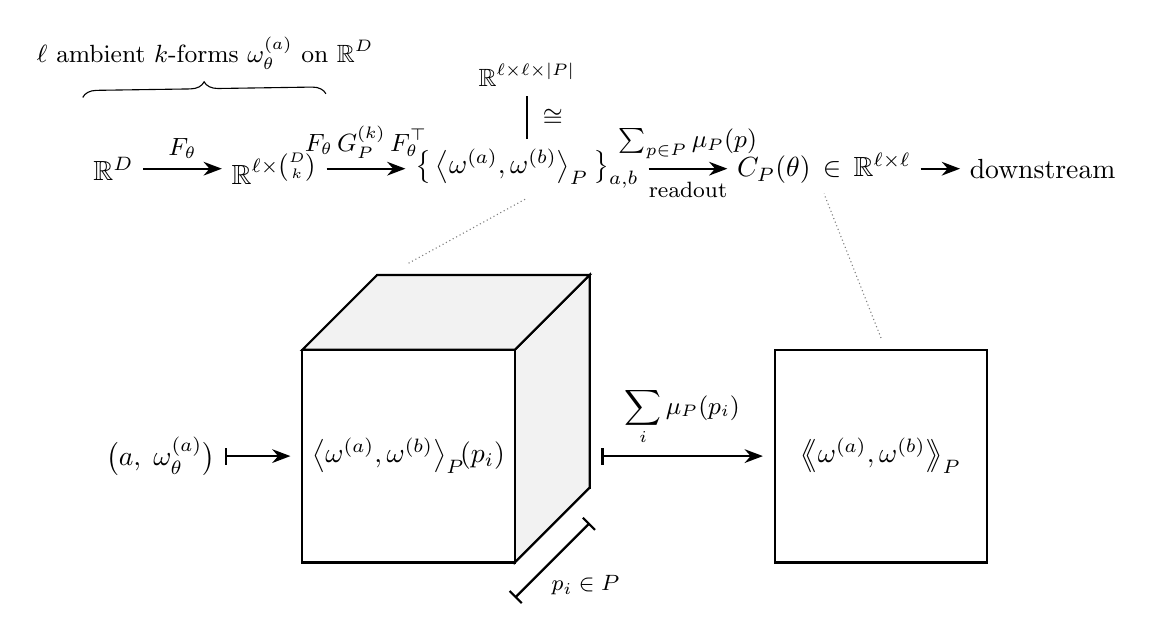
\begin{tikzpicture}[
    >=Stealth,
    arr/.style={->, thick},
    mapsto/.style={|->, thick},
    lbl/.style={font=\small, midway, above},
]

% ============ TOP ROW: PIPELINE ============

\node (RD) {$\mathbb{R}^{D}$};

\node[right=1.0cm of RD] (FRange) {$\mathbb{R}^{\ell \times \binom{D}{k}}$};
\draw[arr] (RD) -- node[lbl] {$F_\theta$} (FRange);

\draw[decorate, decoration={brace, amplitude=5pt, raise=18pt}]
    (RD.north west) -- (FRange.north east)
    node[midway, above=24pt, font=\small]
    {$\ell$ ambient $k$-forms $\omega^{(a)}_\theta$ on $\mathbb{R}^{D}$};

\node[right=1.0cm of FRange] (PerP)
    {$\bigl\{\,\bigl\langle \omega^{(a)}, \omega^{(b)}\bigr\rangle_{P}\,\bigr\}_{a,b}$};
\draw[arr] (FRange) -- node[lbl] {$F_\theta\, G^{(k)}_P\, F_\theta^{\top}$} (PerP);

\node[above=0.55cm of PerP, font=\small] (Shape)
    {$\mathbb{R}^{\ell \times \ell \times |P|}$};
\draw[thick] (PerP) -- node[midway, right=2pt, font=\small] {$\cong$} (Shape);

\node[right=1.0cm of PerP] (CP) {$C_P(\theta)\,\in\,\mathbb{R}^{\ell \times \ell}$};
\draw[arr] (PerP) -- node[lbl] {$\sum_{p\in P}\mu_P(p)$}
    node[below=1pt, midway, font=\footnotesize] {readout} (CP);

\node[right=0.5cm of CP] (task) {downstream};
\draw[arr] (CP) -- (task);

% ============ BOTTOM ROW: CUBE + GRAM MATRIX ============

\def\cx{2.4} \def\cy{-5.0}
\def\cs{2.7}
\def\cd{0.95}

\node at (\cx - 1.8, \cy+0.5*\cs) (input) {$\bigl(a,\; \omega^{(a)}_\theta\bigr)$};

% Back face
\draw[thick, fill=white] (\cx+\cd, \cy+\cd) rectangle +(\cs, \cs);
% Side face
\draw[thick, fill=gray!10]
    (\cx+\cs, \cy) -- +(\cd, \cd) -- +({\cd}, {\cd+\cs}) -- +(0, \cs) -- cycle;
% Top face
\draw[thick, fill=gray!10]
    (\cx, \cy+\cs) -- +(\cd, \cd) -- +({\cd+\cs}, \cd) -- +(\cs, 0) -- cycle;
% Front face
\draw[thick, fill=white] (\cx, \cy) rectangle +(\cs, \cs);

% Label inside cube
\node[font=\normalsize] at (\cx+0.5*\cs, \cy+0.5*\cs)
    {$\bigl\langle \omega^{(a)}, \omega^{(b)} \bigr\rangle_{P}\!(p_i)$};

% p_i line along depth
\coordinate (pLineL) at ($({\cx+\cs}, {\cy}) + (0, -0.45)$);
\coordinate (pLineR) at ($({\cx+\cs+\cd}, {\cy+\cd}) + (0, -0.45)$);
\draw[thick, {|}-{|}] (pLineL) -- (pLineR);
\node[font=\footnotesize, below=2pt, xshift=12pt] at ($(pLineL)!0.5!(pLineR)$) {$p_i \in P$};

% mapsto: form pair -> cube entry
\draw[mapsto] (input.east) -- (\cx-0.15, \cy+0.5*\cs);

% Comparison matrix C_P(theta)
\def\mx{8.4} \def\my{-5.0}
\draw[thick, fill=white] (\mx, \my) rectangle +(\cs, \cs);
\node[font=\normalsize] at (\mx+0.5*\cs, \my+0.5*\cs)
    {$\bigl\langle\!\!\bigl\langle \omega^{(a)}, \omega^{(b)} \bigr\rangle\!\!\bigr\rangle_{P}$};

% sum arrow with weighted readout
\draw[mapsto] (\cx+\cs+\cd+0.15, \cy+0.5*\cs) --
    node[midway, above, font=\small] {$\displaystyle\sum_{i} \mu_P(p_i)$}
    (\mx-0.15, \my+0.5*\cs);

% Dotted alignment between bottom panels and the top-row pipeline
\draw[gray, densely dotted] (\cx+0.5*\cs, \cy+\cs+\cd+0.15) -- (PerP.south);
\draw[gray, densely dotted] (\mx+0.5*\cs, \my+\cs+0.15) -- (CP.south);

\end{tikzpicture}

    \caption{NPF Learning Pipeline.}
    \label{fig:placeholder}
\end{figure}





%\section{Related Work}
%\input{6_related-work}

% \printbibliography



%\section{Practices of \( k \)-Form Comparison (Discrete)}
\section{Discretization}
\label{appendix:B}

The purpose of this appendix section is to investigate in detail the theoretical and practical groundwork for neural point-forms. In Section~\ref{Appendix:subsec:discrete-kfcs} we further discuss the relevant definitions and implementation details used in our experiments, and in Section~\ref{Appendix:Subsec:theory} we prove consistency results justifying these definitions and practices. Future appendices apply this groundwork in experiments.

Throughout this section, $M \subset \mathbb{R}^{D}$ is a \( d \)-manifold with nonvanishing probability density $q \in C^3(M) \cap L^1(M)$, from which a point cloud $P=\{ p_{i} \overset{\text{i.i.d.}}{\sim} q \}_{i=1}^n$ is sampled.

\subsection{Point Form Estimation}
\label{Appendix:subsec:discrete-kfcs}
\label{appendix:B1}

In this subsection, we provide details regarding the definition and implementation of point forms on data. As seen in Appendix~\ref{appendix:A-smooth-review} and the main text, the continuous pipeline relies on three components: the metric \( g \) with which to locally compare \( 1 \)-forms, a formalism extending this construction to the local comparison of general \( k \)-forms, and a measure \( \mu \) against which one may average local comparisons to obtain a global comparison. We elaborate upon the discretization of each notion in turn. 



\subsubsection{Estimating the Carré du Champ From Data}
\label{subsubsec:cdc-estimation-from-data-including-variable-bandwidth-laplacian-contruction}



In this section we assume $M$ potentially noncompact, as we wish to accommodate the possibility that the sampling density $q>0$ can become arbitrarily close to zero. 

\paragraph{Variable-Bandwidth Diffusion Kernels and Laplacians}

One approach to estimating the carré du champ $\Gamma$ on $P$ is to directly estimate a diffusion generator $\Delta$ on \( M \) and from it mimic Equation~\ref{eqn:one-of-many-cdc-identities}.\footnote{There are similar but distinct approaches which bypass intermediate Laplacian estimation, see e.g.~\cite{bamberger2025carr, jonesComputingDiffusionGeometry2026}.} This is generally accomplished by defining a particular transition kernel on the data and examining the ``discrete generator" of a corresponding Markov chain. Our practice and theory both work with the flexible class of \textbf{variable-bandwidth diffusion kernels}, following the construction in~\cite{Berry2016} given by the following sequence of operations:
\begin{enumerate}
    \item Select $\beta < 0.$
    \item Define a ``bandwidth function" \( \rho:M \to \mathbb{R}_{+} \). In the ideal setting, one takes
    \begin{equation}
        \rho(p_i) := q(p_i)^\beta 
    \end{equation} using the true sampling density. 
    \item Select a global bandwidth parameter $\varepsilon > 0$. 
    \item Define the \textit{unnormalized} variable bandwidth kernel 
    \begin{equation}
       K_{\varepsilon}(x,y)=h\left(\frac{\|x-y\|^{2}}{\varepsilon \rho(x) \rho(y)}\right)     \end{equation}for some $h$ with exponential decay. By default, we take $h(u):=e^{-u/4}$. 



    \item Define the unnormalized density estimate
    \begin{equation}
        q_\varepsilon(p_i) = \sum_{j=1}^N \dfrac{K_\varepsilon^{}(p_i,p_j)}{\rho(p_i)^d}.
    \end{equation}
    \item Select a density sensitivity parameter $\alpha > 0.$
    \item Define the symmetric \textit{$\alpha$-density weighted kernel} 
    \begin{equation}
        K_{\varepsilon,\alpha}^{}(p_i, p_j) := \dfrac{{K_\varepsilon}^{}(p_i,p_j)}{q_\varepsilon^{}(p_i)^\alpha q_\varepsilon^{}(p_j)^\alpha}.
    \end{equation}
    \item In order to normalize into a Markov (probability) kernel, first take the row sums
    \begin{equation}
        q_{\varepsilon,\alpha}^{}(p_i) := \sum_{j=1}^N K_{\varepsilon,\alpha}^{}(p_i,p_j),
    \end{equation}
    \item and then define 
    \begin{equation}
        \hat{K}^{}_{\varepsilon,\alpha}(p_i,p_j) := \dfrac{K_{\varepsilon,\alpha}^{}(p_i,p_j)}{q_{\varepsilon,\alpha}^{}(p_i)}.
    \end{equation}
    \item Define the ``discrete diffusion generator"
    \begin{equation} \label{discrete-variable-bandwidth-laplacian}
       L_{P}:= L_{\varepsilon,\alpha,\beta}^{}(p_i,p_j) := \dfrac{ \hat{K}_{\varepsilon,\alpha}^{}(p_i,p_j)-\delta_{ij}}{\varepsilon \rho(p_i)^2} =  \dfrac{ \hat{K}_{\varepsilon,\alpha}^{}(p_i,p_j)-\delta_{ij}}{\varepsilon q(p_i)^{2\beta}}.
    \end{equation} where we have set $\rho = q^\beta$. 
\end{enumerate}

\begin{remark}
The above construction is an instantiation for variable-bandwidth kernels of a general  ``3-kernel procedure" within the diffusion maps literature:
    \begin{enumerate}
        \item An unnormalized variable bandwidth kernel $K_\varepsilon^{}$
        \item An $\alpha$-density weighted kernel $K_{\varepsilon,\alpha}^{}$. 
        \item The row-normalized (Markov) kernel $\hat{K}_{\varepsilon,\alpha}$.
    \end{enumerate} 
    Note that when $\alpha=0$ the second step is skipped. When $\beta = 0$ then the recovered operator equals the classical (fixed-bandwidth) diffusion maps Laplacian \cite{coifman2006diffusion}.
\end{remark}




There are a number of quantities from the idealized discussion above that need to estimated in order to calculate the discrete Laplacian in practice. These are:
\begin{enumerate}
    \item Empirical density estimate $q_0$ of the true sampling density $q$. 
    \item Number of \( k \)-nearest neighbors to use (rather than fully-connected).
    \item Bandwidth choice $\varepsilon$.
    \item Dimension parameter $d$, or estimate thereof. 
\end{enumerate}
We discuss these in turn.

\paragraph{Empirical density estimate} In practice, we do not have access to the ground truth sampling density $q$, so it needs to be estimated. We follow the estimator offered in~\cite{Berry2016}. For each $p_i \in P$, let $I(i,j)$ denote the index of the $j$th nearest neighbor of $p_i$.
Define the local scale
\[
\rho_0(p_i)
:=
\left(
\frac{1}{k_0-1}\sum_{j=2}^{k_0} \|p_i-p_{I(i,j)}\|^2
\right)^{1/2}.
\]
Set
\[
\varepsilon_0^{1/2}
:=
\frac{1}{N}\sum_{i=1}^N \rho_0(x_i),
\qquad
\widetilde{\rho}_0(p_i)
:=
\frac{\rho_0(x_i)}{\varepsilon_0^{1/2}}.
\]

%It is shown in \cite{Berry2016} that \( \rho_{0}=\rho +O(\varepsilon) \) for \( \rho=q^{\beta}  \) defined in terms of the true density \( q \). 


%\paragraph{Berry--Harlim variable-bandwidth construction.}
Now let $\{p_i\}_{i=1}^n \subset \mathbb{R}^D$ be data sampled from a density $q$ on a
$d$-dimensional manifold $M \subset \mathbb{R}^n$. Using the symmetric kernel with local bandwidth $\rho_0$, define
\[
q_0(p_i)
:=
(2\pi)^{-d/2}\frac{1}{\rho_0(p_i)^d\,N}
\sum_{l=1}^N
\exp\!\left(
-\frac{\|x_i-x_l\|^2}{2\,\rho_0(p_i)\rho_0(p_l)}
\right).
\]
Equivalently,
\[
q_0(x_i)
=
(2\pi\varepsilon_0)^{-d/2}\frac{1}{\widetilde{\rho}_0(p_i)^d\,N}
\sum_{l=1}^N
\exp\!\left(
-\frac{\|p_i-p_l\|^2}
{2\varepsilon_0\,\widetilde{\rho}_0(p_i)\widetilde{\rho}_0(p_l)}
\right).
\] %Equation (10) in \cite{Berry2016} implies that this empirical density estimate $q_0$ approximates the true density by
%\begin{equation}
%    q_0(p_i) = q(p_i) + {O}(\varepsilon_0).
%\end{equation}
In \cite{Berry2016} it is shown that choosing \( \rho := q_{0}^\beta \) entails \( \rho=q^\beta + O(\varepsilon) \) with high probability. Our local theory (Sections~\ref{subsubsec:kolmogorov-convergence}-\ref{subsubsec:local-kfc-consistency}) is stated under the assumption \( \rho=q^\beta + O(\varepsilon) \), and thus applies to this empirically-determined bandwidth choice with high probability. 
%\footnote{\todo[global theory will want more guarantees on the estimate of \( q \) itself]} is stated under the assumption \( \rho=q^\beta + O(\varepsilon) \), and thus applies to this empirically-determined bandwidth choice with high probability. \todo[i think this is the thing to say]

 

%Since the theory in \cite{Berry2016} holds assuming that \( \rho=q^{\beta}+O(\varepsilon) \), it holds upon replacing the oracle \( q \) with \( q_{0} \). %It is very likely that much of our own theory in Appendix~\ref{Appendix:Subsec:theory}, being an extension of that in \cite{Berry2016}, does too, even though we work directly with the oracle \( q \) for clarity. \todo[actually let me track this a little bit]



\begin{remark}
The theory in \cite{Berry2016}, and in turn our own (Appendix~\ref{Appendix:Subsec:theory}), are written in terms of the fully connected graph Laplacian. Following \cite{Berry2016}, we use the \( k \)-NN graph as an approximation for efficiency in practice, but note that our forthcoming convergence results are not strictly applicable in this case.
\end{remark}

\paragraph{Notation} To reduce ambiguity, for the remainder of this appendix, we will notate discrete quantities on \( P \) with subscripts tracking the explicit hyperparameters they depend on (such as \( \varepsilon\)) in lieu of the notation \( (\_) _{P}\) adopted in the main text. Similarly, we will variously denote quantities associated to the Riemannian manifold \( (M,g) \) with subscripts \( (\_)_{M} \) or \( (\_)_{g} \), whichever is less ambiguous given the context. Finally, we will employ the `formal pullback' notation \( \langle P^{*} \omega, P^{*} \eta \rangle  \)  to denote the local inner product on discrete \( k \)-forms in order to emphasize that \( \omega, \eta \) live on the ambient space \( \mathbb{R}^{D} \).


\paragraph{Bandwidth estimation}
All of our experiments fix \( \varepsilon=1 \) without further tuning.  
%We perform bandwidth sweeps.. for details, see Section~\toref.

%\todo[In practice, for time constraints, we should just perform bandwidth sweeps $$\varepsilon \in \{2^j \mid -6 \leq j \leq -3 \}$$ with default $\varepsilon = 2^{-5}$. We could alternatively implement a scheme for estimating bandwidth. ]

\paragraph{Dimension estimation}
 The empirical density estimation with theoretical guarantees as described above requires explicit knowledge of the intrinsic dimension \(d\) of the manifold \( M \), and therefore our theory does too. In practice, we estimate intrinsic dimension via local PCA a la~\cite{fukunaga1971algorithm} when it is unknown. 
 %\footnote{For the purposes of estimating \( \Gamma \), one could of course bypass this in practice via an empirical density estimator (or heuristic thereof). However, we again need an empirical density estimate to correct against when defining our density-corrected global inner product, }

%\todo[Not exactly sure what to do about this right now. Do we follow the heiritic of BH based in varepsilon-tuning curve?]






%  \subsubsection{Discrete Local Inner Products}
%  \label{subsubsec:discrete-local-inner-product}

%  \todo[i guess we wait here to find out what actually won't make it into the main text]
% \jake{not sure if there is more to say here, }
\subsubsection{Discrete Inner Products}
\label{subsubsec:discrete-global-inner-product}
%\todo[appendix E.late and maybe other places]



Recall (cf.~\eqref{def:gramfield-global-inner-product}) that in the smooth setting, the global (\( L^2 \)) inner product between restricted \( k \)-forms is given by $$\langle \! \langle \iota ^*\omega,  \iota^* \eta \rangle \! \rangle_{g}=\int_{x \in M} \langle \iota^* \omega,  \iota^* \eta \rangle_{g}(x) \, dV(x) , $$
i.e. the average over $M$ with respect to the volume form. If the sampling density $q$ is taken into account, there is a second inner product $$\langle \! \langle \iota ^* \omega , \iota^*\eta \rangle \! \rangle_{g, q}= \int_{x \in M} \langle \iota^*\omega, \iota^*\eta \rangle_{g}(x) q(x)\, dV(x),  $$
which weighs this average by assigning higher weights to dense regions. Which inner product to emulate in the discrete case depends on whether one would like to classify manifolds or manifolds \textit{with densities}. These correspond to averaging the discrete local inner product $\langle \_, \_ \rangle_{\varepsilon}$ against one of the following discrete measures on $P$:
\begin{enumerate}
    \item (Density-corrected) 
 \begin{equation}
        \langle \! \langle P^*\omega,P^* \eta \rangle \! \rangle_{\varepsilon} := \dfrac{1}{N}\sum_{p_i} \langle \omega ({p_i}), \eta({p_i})\rangle_{\varepsilon} \dfrac{1}{q(p_i)} { \approx \dfrac{1}{N}\sum_{p_i} \langle \omega_{p_i}, \eta_{p_i}\rangle_P \dfrac{1}{q_0(p_i)}}
    \end{equation}
    \item (Non-density corrected)
    \begin{equation}
        \langle \! \langle \omega, \eta \rangle \! \rangle_{\varepsilon,q}:= \dfrac{1}{N}\sum_{p_i} \langle \omega({p_i}), \eta({p_i})\rangle_{\varepsilon}
    \end{equation}
\end{enumerate}

Corollary~\ref{cor:global-continuum-limit} will formalize the validity of this intuition.


\subsection{Consistency Theory for \( k \)FC Discretization}
\label{Appendix:Subsec:theory}


\label{appendix:B2}
% \todo[consistency theory]
% \todo[we reserve the subscript i to index points \( p_{i} \in P \) and the super script \( i \) to index coordinate functions \( x^i \)]
% \todo[i think for \( C_{A} \) and \( C_{B} \) they are actually usually equal to regular numbers like 2 or 4 mostly so maybe we do that?]

% \todo[light overview] \todo[maybe note at some point that A feature of the consistency theory introduced in this section is its generality... it accomodates nonuniform sampling, noncompactness, variable-bandwidths, is largely agnostic to the implementation pipeline, is provably insensitive to cetain parameter choicees, etc... basically it handles the exact pipeline from in practice, no idealizations except perhaps (1) knn truncation (2) knowledge of intrinsic dimension \( d \) just realizing how much easier life would get if  ]




% {\color{red}
% \begin{itemize}

%     \item optimal choice of \( \alpha \) the minimize the third term in \( \delta \)? (constraint: \( c_{2}<0, c_{1} \geq 0\))
%     \item I elected to take the expositional approach of not locally redefining things in the statements of results, but maybe that is unwise for a paper where people go to reference stuff rather than read chronologically like a textbook. for the main three results we have can be more thorough
    
% \end{itemize}
% }

The goal of this subsection is to prove a (formal version of) Theorem~\ref{ithm:main-text-continuum-limits} from the main text and examine its consequences. Our central result, from which Theorem~\ref{ithm:main-text-continuum-limits} is derived, is as follows. 


\newtheorem*{theorem*}{Theorem~\ref{thm:locla-consistency-estimate} (Informal)} \begin{theorem*}
    Let $p_{i} \in M$, $\omega,\eta \in \Omega^{k}(\mathbb{R}^{D})$. With high probability, $$\langle P^{*}\omega, P^{* }\eta \rangle_{\varepsilon, n}(p_{i})= \langle \iota^{*}\omega, \iota^{*}\eta \rangle_{g}(p_{i}) + O_{k, \omega ,\eta,p_{i}} \left(  \varepsilon, \frac{q(p_{i})^{(1-d \beta)/2}}{\sqrt{ n } \varepsilon^{2+d/4}}, (1+2\max_{ \ell }  |x^{\ell}(p_{i})|) \frac{q(p_{i})^{-c_{2}}}{\sqrt{ n } \varepsilon^{1/2+d/4}}  \right)  $$
for a constant \( c_{2} \) depending on \( \alpha, \beta \), and this estimate can be made uniform in $p_{i}$ provided $M$ is compact. 

\end{theorem*}

Our theory diverges from implementation in two main ways. First, it assumes fully connected kernel graphs, whereas the implementation uses \(k\)-NN truncation for efficiency. Certifying compatibility with \( k \)-NN truncation is nontrivial and left for future work.
%The second is that it assumes access to the oracle density \( q \), although we will see that relaxing Theorem~\ref{thm:locla-consistency-estimate} to hold for any estimate \( \hat{q} \) accurate to order-\( \varepsilon \) (such as the estimate \( q_{0} \) used in our experiments) is likely straightforward. 
% Second, it requires knowledge of \( d=\dim M \). These caveats aside, a feature of our theory is its faithfulness to practice: our results treat nonuniform sampling, unknown \( q \), noncompactness, and variable bandwidths and are hyperparameter-insensitive. 
Second, it assumes knowledge of the intrinsic dimension \(d=\dim M\). Beyond these two assumptions, a feature of our theory is its faithfulness to practice. Our results treat nonuniform sampling from an unknown density, variable bandwidths, and explicit finite-sample dependence upon (and provable insensitivity to) normalization parameters. 

%Subject to these standard assumptions, the theory still captures several practical features: nonuniform sampling, variable bandwidths, and explicit finite-sample dependence on normalization parameters. 



% Throughout this section, we assume \( \rho=q^\beta + O(\varepsilon) \). This holds with high probability e.g. for the empirical \( \rho \) used in our experiments (cf. Section~\ref{subsubsec:cdc-estimation-from-data-including-variable-bandwidth-laplacian-contruction}) \cite{Berry2016}. In particular, we do not require the true sampling density \( q \) to be known to achieve consistency.

Throughout this section, we assume \( \rho=q^\beta + O(\varepsilon) \). This holds with high probability e.g. for the empirical \( \rho \) used in our experiments (cf. Section~\ref{subsubsec:cdc-estimation-from-data-including-variable-bandwidth-laplacian-contruction}) \cite{Berry2016}. In particular, our central consistency result (Theorem~\ref{thm:locla-consistency-estimate}) does not require the true sampling density \( q \) to be known. 

%For the local pairing results, oracle access to \(q\) is not required if the empirical bandwidth satisfies \( \rho=q^\beta + O(\varepsilon) \). Density-corrected consistency have different proof obligations. 


% \paragraph{other} 
% Other caveats on the results of this section include:
% - fully-connected (in practice one truncates knn)
% - global inner products on noncompact manifolds
% - data might not actually be manifolds... things like locally manifold/union of manifold data we don't treat
% - we do not assume any noise in the sampling procedure (indeed, how does noise affect the diffusion maps theory?)



% (actually just here put the "caveats" section that rn is way below?



% \subsubsection{\todo[i am just collecting random stuff in this subsubsection right now]}

%\( q \in C^3(M) \cap L^1(M) \cap L^\infty(M) \)

%to specialized $\rho=q^{\beta }+O(\varepsilon)$*
%- use general shape function $h$ like they do, $k_{\varepsilon,\beta}=h( \frac{\|x-y\|^{2}}{\varepsilon \rho(x) \rho(y)} )$  for $\rho=q^{\beta}+O(\varepsilon)$.  this most just to keep track of $m$

% $\overline{J}_{i} = \overline{J}(i)= \frac{1}{n-1} \sum_{j \neq i}J_{i}(j)$ for \( J_{i}\) a function of \( j \in [n] \) .

% {\color{red}
% Originally (Theorem 1 of BH), it is written
% \begin{align}
% (S_{\varepsilon, \alpha, \beta} f)(p_{i})=\sum_{j=1}^{n} f(p_{j}) P_{\varepsilon, \alpha, \beta}(p_{i}, \{ p_{j} \})&=\frac{\sum_{j=1}^{n} \overbrace{ f(p_{j}) {k_{\varepsilon,\alpha, \beta}(p_{i}, \{ p_{j} \})} }^{ =:F_{i}(p_{j}) }}{\sum_{j=1}^{n} \underbrace{ k_{\varepsilon. \alpha, \beta}(p_{i}, \{ p_{j} \} }_{ =: G_{i}(p_{j}) })} .
% \end{align}
% But note that Berry-Harlim update the definitions $F_{i}, G_{i}$ on page $2 2$ as
% - $F_{i}(p_{j})\leftarrow aF_{i}(p_{j})$  
% - $G_{i}(p_{j})\leftarrow aG_{i}(p_{j})$
% where $a:=n \varepsilon^{d/2}q_{\varepsilon, \beta}(p_{i})^{\alpha}$. We'll use these new notatin from now on.  The modification is immaterial because in the ratio they care about everything else will cancel (some factors for obvious reasons, others less obvious ones but they discuss it). In particular, we still have\footnote{We write '$\approx$' because notation $\overline{J}$ is strictly speaking leave-one-out average rather than the true averages used to define $S_{\varepsilon, \alpha, \beta}$. } 
% $$\frac{\overline{F}_{i}}{\overline{G}_{i}}\approx S_{\varepsilon, \alpha, \beta }f (p_{i})$$
% and so $\check{L}f(p_{i})=\frac{S_{\varepsilon, \alpha, \beta}f(p_{i})-f(p_{i})}{\varepsilon} \approx  \frac{\frac{\overline{F}_{i}}{\overline{G}_{i}}- f(p_{i})}{\varepsilon}$, whence

% $$L_{\varepsilon, \alpha, \beta}f(p_{i})=\frac{1}{ m \rho(p_{i})^{2}} \check{L} f(p_{i}) \approx \frac{1}{m \rho(p_{i})^{2}\varepsilon}\left(  \frac{\overline{F}_{i}}{\overline{G}_{i}}- f(p_{i})  \right).$$
% Replacing the empirical averages with population expectations, we make the definition
% $$\mathcal{L}_{\varepsilon, \alpha, \beta }f(p_{i}):=\frac{1}{m \rho(p_{i})^{2}} \check{\mathcal{L}}f(p_{i}), \text{ where }\check{\mathcal{L}}f(p_{i}):=\frac{\frac{\mathbb{E}[F_{i}]}{\mathbb{E}[G_{i}]}- f(p_{i})}{\varepsilon}.$$  



% }

% Also define $\varepsilon^{d/2}H_{j}(x_{\ell}):=\overbrace{  \frac{1}{\rho(p_{j})^{d}} k_{\varepsilon, \beta}(p_{j}, p_{\ell}) }^{ \ell \text{th}  \text{ term  of }q_{\varepsilon, \beta}(p_{j}) }$, so that $\overline{H}_{j}=\frac{1}{n-1} \varepsilon^{-d/2}(q_{\varepsilon, \beta}(p_{j})- H_{j}(p_{j}) \varepsilon^{d/2}) \approx \frac{\varepsilon^{-d/2}}{n}q_{\varepsilon, \beta}(p_{j})$. 



\subsubsection{Kolmogorov Convergence}


\label{subsubsec:kolmogorov-convergence}
The theory of variable-bandwidth diffusion kernels is supported by the following result, due to Berry and Harlim~\cite{Berry2016}. 
\begin{proposition}[\cite{Berry2016}, Corollary \( 1 \)]
\label{prop:BH-cor1}
Assume \( \rho=q^\beta  + O(\varepsilon)\). Let \( p_{i} \in M \), \( f \in L^2 \cap C^3(M) \). Define $$\delta_{\varepsilon, n, \alpha, \beta, f}(p):=\max \left(\varepsilon, \frac{q(p_{i})^{(1- d \beta) / 2}}{\sqrt{ n }\varepsilon^{2+d/4}}, \frac{\|\nabla f(p_{i})\| q(p_{i})^{-c_{2}}}{\sqrt{ n } \varepsilon^{1/2+d/4}}\right).$$
With high probability,
$$L_{\varepsilon, \alpha, \beta}f(p_{i})= \mathcal{L} _{\alpha, \beta}+ O\big(\delta_{\varepsilon, n, \alpha, \beta ,f}\big)(p_{i}) ,$$
where $$\mathcal{L}_{\alpha, \beta}= \frac{1}{q^{c_{1}}} \operatorname{div}(q^{c_{1}} \nabla f) = \Delta f +  c_{1} \nabla f \cdot \frac{\nabla q}{q}$$
for $c_{1}=2-2\alpha + d \beta + 2 \beta$ and $c_{2}=1 / 2 - 2\alpha + 2d \alpha + d \beta / 2 + \beta$. 

\end{proposition}

The Laplacian \( \Delta \) on \( M \) is recovered provided \( c_{1}=0 \), for instance when \( \alpha= \frac{1}{2} - \frac{d}{4} \), \( \beta=- \frac{1}{2} \). 

\begin{remark}
\label{remark:BH-purpose}
    If \( q \) is not bounded below (i.e. sampling is permitted to be arbitrarily sparse), then \( \delta_{\varepsilon, n, \alpha, \beta, f}  \) can explode as \( q \to 0 \) provided \( c_{2} > 0 \). The fixed-bandwidth case \( \beta=0 \) \textit{forces} \( c_{2} >0\); this concretely motivates variable-bandwidth kernels. Note that this scenario cannot occur if \( M \) is compact, since then \( q \) must be bounded below.\footnote{We will exploit this simple principle at length in Section~\ref{Appendix:Subsec:theory}.} While convergence results akin to Proposition~\ref{prop:BH-cor1} have been established for compact \( M \) since~\cite{coifman2006diffusion}, and bare convergence results in the variable-bandwidth case since~\cite{ting2010analysis}, the focus of \cite{Berry2016} is the explicit characterization of the bound in terms of the parameters \( \alpha, \beta \) and the true sampling density \(  q\) in the potentially noncompact case. Other heuristic justifications for variable-bandwidth diffusion kernels include:
    \begin{enumerate}
        \item They are less sensitive to \( \varepsilon \) than their fixed-bandwidth counterparts;
        \item They more effectively and transparently account for density.
    \end{enumerate}
\end{remark}

\begin{remark}
\label{rmk:whp-explanation}
   {By "with high probability", we mean the conclusion of Proposition~\ref{prop:BH-cor1} holds on an event $E_{\varepsilon, n, i , f}=A_{\varepsilon, n} \cap B_{\varepsilon, n, i ,f}$ satisfying}
\begin{equation}
\mathbb{P}(E_{\varepsilon, n, i, f}^{c}) \leq C_A n  \, e^{- c_{A}n \varepsilon^{4+ d/ 2}}+C_{B}e^{-c_{B,i, f}n \varepsilon^{3+d/2}}
\end{equation}
{for some constants $C_{A},C_{B},c_{A},c_{B,i, f}>0$ corresponding to the latter two terms of \( \delta_{\varepsilon, n, \alpha, \beta, f} \).}\footnote{Specifically, the event $A_{\varepsilon, n}$ corresponds to the second term $\frac{q(p_{i})^{(1- d \beta)/2}}{\sqrt{ n }\varepsilon^{2+ d/ 4}}$ of $\delta_{\varepsilon, n, \alpha, \beta, f}(p_{i})$ uniformly in $i$ and independent of $f$, while $B_{\varepsilon, n, i, f}$ corresponds to the third term $\frac{\|\nabla f(p_{i})\| q(p_{i})^{-c_{2}}}{\sqrt{ n } \varepsilon^{1/2+d/4}}$. (The first term $\varepsilon$ of $\delta_{\varepsilon, n, \alpha, \beta, f}(p)$ is deterministic, cf. Appendix A of~\cite{Berry2016}.); because they can be black-boxed without loss of continuity, we further defer a detailed derivation of these bounds to Appendix~\ref{subsubsec:the-bh-good-event}.}

%\kelly{please get rid of the tiny font its driving me insane aha}\jake{i evicted it to Section~\ref{subsubsec:the-bh-good-event}, what do you think?}


\end{remark}

We are ultimately interested in estimating maps built from quantities of the form \( L_{\varepsilon, \alpha, \beta} f\) as \( f \) \textit{varies} over some finite function family \( F \). Toward this end, we collect the following corollary of Proposition~\ref{prop:BH-cor1}.

%\todo[i have not been careful about \( L^2(M) \) vs \( L^2(M,q) \), so should go through later and correct that]
\begin{lemma}[Uniformizing in \( f \)] Let \( p_{i} \in M. \). Given ${F} \subset C^{3}(M) \cap L^{2}(M, q) $ finite, define $$\delta_{\varepsilon, n, \alpha, \beta, {F}}(p_{i}):=\max_{f \in {F}} \{ \delta_{\varepsilon, n, \alpha, \beta, f}(p_{i})\}.$$
 With high probability, 
    \begin{equation}
        L_{\varepsilon, \alpha, \beta}f(p_{i})= \mathcal{L} _{\alpha, \beta}f(p_{i})+ O\big(\delta_{\varepsilon, n, \alpha, \beta ,F}(p_{i})\big) \text{ for all }f \in F.
        \label{eqn:unif-f}
    \end{equation}
    Specifically, the above holds on an event \( E_{\varepsilon, n, i} \) with failure probability \( \mathbb{P}(E_{\varepsilon, n, i}^{c})  \leq C_{A} n e^{-c_{A}n \varepsilon^{4+d/2}}+C_{B} \# F e^{-c_{B, i, F}n \varepsilon^{3+d/2}}\).
    \label{lemma:uniformizing-in-f}
\end{lemma}

\begin{proof}
    Importing the notation and context of Remark~\ref{rmk:whp-explanation}, we see that the claim holds on the event $E_{\varepsilon, n, i}:=A_{\varepsilon, n} \cap \bigcap_{f \in F}^{}B_{\varepsilon, n, i , f}$, whose failure probability may be estimated $$\mathbb{P}(E^{c}_{\varepsilon, n, i}) \leq \mathbb{P}(A_{\varepsilon, n}^{c})+ \sum_{f \in F}\mathbb{P}(B^{c}_{\varepsilon, n,i,f})\leq C_{A} n e^{-c_{A}n \varepsilon^{4+d/2}}+C_{B} \# F e^{-c_{B, i}n \varepsilon^{3+d/2}},$$
where $c_{B,i}=\min_{f \in F} c_{B,i,f}$. 
\end{proof}


At times, we will also be interested in statements holding uniformly on \( P \). A sufficient condition is compactness of \( M \).\footnote{We reiterate that compactness of \( M \) is not a standing assumption of the present section; indeed, Lemma~\ref{lemma:uniformizing-in-i-with-compactness} will not see heavy use until the global convergence proofs of Section~\ref{subsubsec:global-kfc-consistency}. }
\begin{lemma}
Assume in addition that $M$ is compact. Let $F \subset C^{3}(M) \cap L^{2}(M,q)$ be finite, and define
\begin{equation}
\overline{\delta}_{\varepsilon, n, \alpha, \beta, F}:=\sup_{p \in M}\delta_{\varepsilon,n,\alpha, \beta, F}(p).
\end{equation}
Then $\overline{\delta}_{\varepsilon, n, \alpha, \beta ,F}<\infty$, and with high probability,
\begin{equation}
L_{\varepsilon, \alpha, \beta}f(p_{i}) = L_{\alpha, \beta}f(p_{i})+O(\overline{\delta}_{\varepsilon, n, \alpha, \beta, F}) \text{ for all }i \in [n] \text{ and }f \in F.
\end{equation}
Specifically, the above holds on an event $E_{\varepsilon, n}$ with failure probability
\begin{equation}
\mathbb{P}(E_{\varepsilon, n}^{c}) \leq C_{A} n e^{-c_{A}n \varepsilon^{4+d/2} }+C_{B} n \# F e^{-c_{B}n\varepsilon^{3+d/2}}.
\end{equation}
\label{lemma:uniformizing-in-i-with-compactness}
\end{lemma}


\begin{proof}

Import the notation and context of Remark~\ref{rmk:whp-explanation} and Lemma~\ref{lemma:uniformizing-in-f}. 

Since $M$ is compact and $q>0$ is continuous, there exist constants $q_{\text{min}}$, $q_{\text{max}}$ such that $0<q_{\text{min}} \leq q \leq q_{\text{max}}$. Since $F \subset C^{3}(M)$, each $\|\nabla f\|_{\infty}<\infty$, and then since $F$ is finite, $Z_{F}:=\max_{f \in F}\|\nabla f\|_{\infty}<\infty$.  Therefore $\delta_{\varepsilon, n, \alpha, \beta, F}:M \to \mathbb{R}$ is bounded on $M$, hence $\overline{\delta}_{\varepsilon, n, \alpha, \beta, F}<\infty$, and moreover the pointwise constant $c_{B,i}=\min_{f \in F} c_{B, i, f}$, $c_{B,i,f}=c_{B,i,f}(\hat{a}_{2}, c_{2}, c, \|\nabla f(p_{i})\|, q(p_{i}))$, is uniformly bounded in $i$, say, by some $0<c_{B}\leq \inf_{i \in [n]}c_{B,i}$. 

We see that the claim holds on the event $E_{\varepsilon, n}:= \bigcap_{i=1}^{n} E_{\varepsilon , n, i}=A_{\varepsilon, n} \cap \bigcap_{i=1}^{n}B_{\varepsilon, n, i}$, whose failure probability may be estimated
\begin{align}
\mathbb{P}(E_{\varepsilon, n}^{c})&\leq \mathbb{P}(A_{\varepsilon, n}^{c})+ \sum_{i=1}^{n} \mathbb{P}(B_{\varepsilon, n, i}^{c}) \\
&\leq C_{A}n e^{-c_{A}n \varepsilon^{4+d/2}}+C_{B}n\# F e^{-c_{B}n \varepsilon^{3+d/2}}
\end{align}
where we have used Lemma~\ref{lemma:uniformizing-in-f}. Since $\delta_{\varepsilon, n ,\alpha, \beta, F}(p_{i})\leq  \overline{\delta}_{\varepsilon, n , \alpha, \beta, F},$ the claimed uniform error follows. 

\end{proof}




\subsubsection{Carré du Champ Consistency}
\label{subsubsec:cdc-consistency}
An emerging paradigm in geometric data analysis leverages the convergence of the Laplacian \( \Delta \) to approximate the Riemannian metric $g$ of a `submanifold' specified through point cloud data \cite{giannakis-berry2020,jones2024diffusiongeometry}. Access is provided via the carré du champ identity
\begin{equation}
    \Gamma_{}(f,h)(p) := \Big( f \Delta_M h + h \Delta_M f - \Delta_M(fh)\Big)(p) = \langle df,dh\rangle_g(p)
    \label{eqn:one-of-many-cdc-identities}
\end{equation} characterizing the metric \( g \) in terms of \( \Delta \) (See Appendix~\ref{app:background-diff-forms}). The work~\cite{jones2026manifolddiffusiongeometrycurvature} applies Proposition~\ref{prop:BH-cor1} to consistently estimate \( \Gamma \) on compact \( M \). We expand the brief argument provided there to examine the roles of \( \alpha \), \( \beta \), and noncompactness. Put \[
2\Gamma_{\varepsilon, \alpha, \beta}(f,h):=\hat{f} L_{\varepsilon, \alpha, \beta}\hat{h} + \hat{h}L_{\varepsilon, \alpha, \beta}\hat{f}-L_{\varepsilon, \alpha, \beta}(\hat{f}\hat{h}),
\]
where $\hat{f}:=P^{*}f$, $\hat{h}=P^{*}h$. 
\begin{corollary}[Based on~\cite{jones2026manifolddiffusiongeometrycurvature}, Corollary 3.2]
\label{cor:cdc-consistency}
Let \( p_{} \in M \), and assume \( F:= \{ f,h, fh \}  \subset C^{3}(M) \cap L^{2}(M,q) \). With high probability, 
% \[
% \Gamma_{\varepsilon, \alpha, \beta}(f,h)(p_{i})= \langle df, dh \rangle_{g}(p_{i}) + O\big(\delta_{\varepsilon,n, \alpha, \beta, {F}:=\{ f,h, fh \}}(p_{i})\big) .
% \]

\[
\Gamma_{\varepsilon, \alpha, \beta} (f, h)(p_{i}) = \langle df, dh \rangle_{g} (p_{i}) + O \big( ( 1 + |f(p_{i})| + |h(p_{i})| ) \delta_{\varepsilon, n, \alpha, \beta, F}(p_{i}) \big).
\]

Specifically, the above holds on an event \( E_{\varepsilon, n, i} \) with failure probability \( \mathbb{P}(E_{\varepsilon, n, i}^{c})  \leq C_{A} n e^{-c_{A}n \varepsilon^{4+d/2}}+C_{B} \# F  e^{-c_{B, i, F}n \varepsilon^{3+d/2}}\).

\begin{remark}
    If in fact \( f,h \in L^\infty (M) \) (such as when \( M \) is compact), then automatically \( f h \in C^3(M) \cap L^2(M) \) and Corollary~\ref{cor:cdc-consistency} applies to produce 
\[
\Gamma_{\varepsilon,\alpha,\beta}(f,h)(p_i)
=
\langle df,dh\rangle_g(p_i)
+
O\!\left(
\varepsilon,\,
\frac{q(p_i)^{(1-d\beta)/2}}{\sqrt n\,\varepsilon^{2+d/4}},\,
\frac{\bigl(\|f\|_\infty+\|h\|_\infty+\|\nabla f(p_i)\|+\|\nabla h(p_i)\|\bigr)\,q(p_i)^{-c_2}}
{\sqrt n\,\varepsilon^{1/2+d/4}}
\right)
\]
with (the same) high probability. Upon setting \( \alpha=\frac{1}{2}-\frac{d}{4} \), \( \beta=-\frac{1}{2} \), this statement specializes to recover Corollary 3.2 in~\cite{jones2026manifolddiffusiongeometrycurvature}. 

\end{remark}


\end{corollary}

% \begin{proof}
% The continuum operator \( \mathcal{L}_{\alpha, \beta} \) consists of a diffusion term \( \Delta \) and a drift term $c_{1} \frac{\nabla q}{q} \cdot \nabla$. The carré du champ constructed via \( \Delta \), by~\toref[standard cdc identity from way earlier], recovers \( \langle df, dh \rangle  _{g}\). The carré du champ constructed via $c_{1} \frac{\nabla q}{q} \cdot \nabla$, 
%  \begin{equation} 
%     \Gamma_{ c_1 \nabla q/q \cdot \nabla} (f,h)(p) =c_1 \dfrac{\nabla q}{q} \Big(  f \nabla h + h \nabla f - \nabla(fh) \Big)(p) ,
%     \end{equation}
% is zero by the Leibniz rule for \( \nabla \). The event fails with the stated probability by Lemma~\ref{lemma:uniformizing-in-f}, which applies because \( f,h \in L^\infty(M) \) (so that \( fh \in L^2(M) \)). 

% \todo[need to relax the conditions ]
% \end{proof}

Applying Lemma~\ref{lemma:uniformizing-in-f} to $F$ produces an event $E_{\varepsilon, n ,i}$ with the stated failure probability on which $$L_{\varepsilon, \alpha, \beta}f'(p_{i}) = \mathcal{L}_{\alpha, \beta}f'(p_{i}) +O(\overbrace{ \delta_{\varepsilon, n, \alpha, \beta, F}(p_{i}) }^{ =: \delta_{F}(p_{i}) }) \text{ for all } f' \in F.$$
We have \begin{align}
2 \Gamma_{\varepsilon, \alpha, \beta}(f,h)(p_{i}) &= f(p_{i}) [\mathcal{L}_{\alpha, \beta}h(p_{i}) + O\big(\delta_{F}(p_{i})\big)] + h(p_{i})[\mathcal{L}_{\alpha, \beta}f(p_{i})+O\big( \delta_{F}(p_{i}) \big)] - \mathcal{L}_{\alpha, \beta}(fh)(p_{i})+O\big( \delta_{F}(p_{i}) \big) \\
&= 2 \Gamma_{\mathcal{L}_{\alpha, \beta}} (f, h)(p_{i}) + O \big ( (1 + |f(p_{i})|+|h(p_{i})|) \delta_{F}(p_{i}) \big).
\end{align}
where $\Gamma_{\mathcal{L_{\alpha, \beta}}}$ is the carré du champ associated to the continuum Kolmogorov operator $\mathcal{L_{\alpha, \beta}}$. In fact, we claim $\Gamma_{\mathcal{L}_{\alpha, \beta}}(f, h)=\underbrace{ \langle df, dh \rangle_{g} }_{ \Gamma(f,h) }$, the carré du champ~\eqref{eqn:one-of-many-cdc-identities} on $(M,g)$. Indeed, $\mathcal{L}_{\alpha, \beta}$ consists of a diffusion term $\Delta$ and a drift term $c_{1} \frac{\nabla q}{q} \cdot \nabla$. The carré du champ constructed via \( \Delta \) recovers \( \langle df, dh \rangle  _{g}\). The carré du champ constructed via $c_{1} \frac{\nabla q}{q} \cdot \nabla$, 
 \begin{equation} 
    \Gamma_{ c_1 \nabla q/q \cdot \nabla} (f,h)(p) =c_1 \dfrac{\nabla q}{q} \Big(  f \nabla h + h \nabla f - \nabla(fh) \Big)(p) ,
    \end{equation}
is zero by the Leibniz rule for \( \nabla \). 

\begin{remark}[Parameter choices]
We see the parameters \( \alpha, \beta \) do not affect the limiting form, only rates (through their interaction with \( q \)). It is suggested in~\cite{Berry2016} to take \( \beta=-\frac{1}{2} \). From there, \( \alpha \) only has to be chosen to produce \( c_{2}<0 \) (so that \( \delta_{\varepsilon, n ,\alpha, \beta, F} \) does not explode in sparsely sampled regions where \( q \) is small, cf. Remark~\ref{remark:BH-purpose}). A sufficient choice is just \( \alpha=0 \). This suggests that \textit{\( \alpha \)-normalization is not necessary to do diffusion geometry}, although rigorous experimentation to confirm or deny such a hypothesis is tangential to the scope of this work and hence omitted. 
%Two other relatively canonical choices of \( (\alpha, \beta) \) correspond to 
        % \begin{equation} 
        %     c_1 = 0 \Rightarrow \alpha = -1/2-d/4 \Rightarrow \mathcal{L}_{\alpha,\beta} = \Delta_M + \dfrac{\nabla q}{q} 
        % \end{equation} or
        % \begin{equation}
        %     c_1 = 1 \Rightarrow \alpha =  -d/4 \Rightarrow \mathcal{L}_{\alpha,\beta} = \Delta_M.
        % \end{equation} Since neither of choices affect the CDC, however, we default to the more basic $\alpha = 0$.
    \label{rmk:parameter-choices}
\end{remark}

\subsubsection{Consistency of the Gram Fields \( G^{(k)} \)}
\label{subsubsec:tangential-projector-consistency}
% \todo[i am not sure if we want Appendix E.4 (tangential projectors in the smooth category) of the ideating document right here in or Appendix A] 


For the remainder of this appendix subsection (Appendix~\ref{appendix:B2}), we suppress \( \alpha \) and \( \beta \) from the notation to emphasize that our results depend on them only by way of finite-sample bounds rather than limiting operators (cf. Remark~\ref{rmk:parameter-choices}). Officially, the norm \( \|A\| \) of a matrix \( A \) in this section is the max-norm, although our estimates would hold for any other norm as well due to finite-dimensionality. 

\begin{proposition}[tangential projector consistency]

Let $p \in M$. Assume that for all $i,j \in[D]$, $\{ x^{i}|_{M}, x^{j}|_{M}, x^{i}x^{j} |_{M} \} \subset C^{3}(M) \cap L^{2}(M,q)$. Set $F:=\{ x^{i} |_{M} \}_{i=1}^{D} \cup \{ x^{i}x^{j} |_{M} \}_{1 \leq i \leq j \leq D} \subset C^{3}(M) \cap L^{2}(M)$. Define \[
\mathfrak{e}_{\varepsilon, n}(p):=\max \{  \varepsilon, \frac{q(p)^{(1-d \beta)/2}}{\sqrt{ n } \varepsilon^{2+d/4}}, (1+2\max_{1 \leq \ell \leq D}  |x^{\ell}(p)|) \frac{q(p)^{-c_{2}}}{\sqrt{ n } \varepsilon^{1/2+d/4}}  \}
\]. With high probability,  

\[
\| G_{M}(p) - G_{\varepsilon, n}(p)  \|_{} = O( \mathfrak{e}_{\varepsilon, n}(p) ),
\]
that is, 

$$\big(G_{\varepsilon, n}(p)\big)^{ij}=G ^{ij}(p)+O( \mathfrak{e}_{\varepsilon, n}(p) ) \text{ for all }i,j \in [D] .$$

Specifically, the above holds on an event $E_{\varepsilon, n,p}$ with failure probability $$\mathbb{P}(E_{\varepsilon, n, p}^{c}) \leq C_{A} n e ^{-c_{A}n \varepsilon^{4+d/2}}+ \frac{D(D+3)}{2} C_{B}e^{-c_{B, i, F}n \varepsilon^{3+d/2}}$$
\label{prop:tangential-projector-consistency}
\end{proposition}
%We observe that this bound is uniform over the pairings of coordinate functions $(x^i)$, and so works uniformly over entries of $G_{P}(p)$. 
The bound above works uniformly over all entries of $G_{\varepsilon, n}^{(k)}(p)$ up to a $k$-dependent constant:

\begin{corollary}[k$th$ tangential projector consistency]
Fix assumptions and notation as in Proposition~\ref{prop:tangential-projector-consistency}, and let \( k \geq 1 \). With high probability,
$$\|G^{(k)}_{M}(p)-G^{(k)}_{\varepsilon, n}(p)\| \leq R^{(k)}_{\varepsilon, n}(p),$$
where $|R^{(k)}_{\varepsilon, n}(p)|\lesssim k!\big( (1+{e}_{\varepsilon, n}(p))^{k}-1\big)^{}$ and $e_{\varepsilon,n}(p)$ is $O(\mathfrak{e}_{\varepsilon,n}(p))$. It follows that $$\|G_{M}^{(k)}(p) - G_{\varepsilon, n}^{(k)}(p)\|=O_{k}(\mathfrak{e}_{\varepsilon, n}(p)).$$

Specifically, the above holds on the same event \( E_{\varepsilon, n ,p} \) as Proposition~\ref{prop:tangential-projector-consistency}. 



\label{cor:kth-tangential-projector-consistency}
\end{corollary}

\begin{remark}
    Assuming the data is mean-centered, this implies an intuitive (although less tight) bound in terms of the diameter of $M$. 
\end{remark}



\begin{proof}[Proof of Proposition~\ref{prop:tangential-projector-consistency}]
Set $F:=\{ x^{i} |_{M} \}_{i=1}^{D} \cup \{ x^{i}x^{j} |_{M} \}_{1 \leq i \leq j \leq D} \subset C^{3}(M) \cap L^{2}(M)$. 
Applying Lemma~\ref{lemma:uniformizing-in-f} to the finite family \( F \) produces an event
\(E_{\varepsilon,n,p}\) with \[\mathbb P(E_{\varepsilon,n,p}^c)\leq C_A n e^{-c_A n\varepsilon^{4+d/2}}+\frac{D(D+3)}2\,C_B e^{-c_{B,p,F_{}}n\varepsilon^{3+d/2}}
\]
on which, for all \( i, j \in [D] \), the operators
\( L_{\varepsilon,\alpha,\beta}(x^i|_M)(p), L_{\varepsilon,\alpha,\beta}(x^j|_M)(p), L_{\varepsilon,\alpha,\beta}(x^i x^j|_M)(p) \) simultaneously satisfy the estimate~\eqref{eqn:unif-f}. Applying the estimates from Lemma~\ref{lemma:uniformizing-in-f} yields
\[(G_{\varepsilon, n}(p))^{ij}=\langle dx^i,dx^j\rangle_g(p)+O\left(\varepsilon, \frac{q(p)^{(1-d\beta)/2}}{\sqrt n\varepsilon^{2+d/4}}, \frac{\Xi(p)\,q(p)^{-c_2}}{\sqrt n\varepsilon^{1/2+d/4}}\right),
\] where we have used pullback naturality to obtain $\Gamma_{M}(\iota^{*}x^{i}, \iota^{*}x^{j})=\langle \iota^{*}dx^{i}, \iota^{*}dx^{j} \rangle$ and 
\[
\Xi(p):=\max\Bigl\{\|\overbrace{ \nabla(x^i|_M)(p)\| }^{ \leq 1 },\overbrace{ \|\nabla(x^j|_M)(p)\| }^{ \leq 1 },\overbrace{ \|\nabla(x^i x^j|_M)(p)\| }^{=\overbrace{ \| x^{i} \nabla(x^{j} |_{M}) +x^{j} \nabla(x^{i} |_{M}) \| }^{ \leq 1 + 2 \max_{\ell \in [D]}|x^{\ell}(p)| } }\Bigr\}\leq 1+2 \max_{\ell \in [D]}|x^{\ell}(p)|. 
\]
\end{proof}



\begin{proof}[Proof of Corollary~\ref{cor:kth-tangential-projector-consistency}]
The proof is combinatorial. Assume the event \( E_{\varepsilon, n, p} \) from the proof of Proposition~\ref{prop:tangential-projector-consistency} holds. Obtain $C>0$ such that, on $E_{\varepsilon, n, p}$, 
$$|\big( G_{\varepsilon, n}(p) \big)^{ij} - \big(G_{M}(p)\big)^{ij}| \leq e_{\varepsilon, n}(p):= C \max \left\{ \varepsilon, \frac{q(p)^{(1-d \beta)/2}}{\sqrt{ n } \varepsilon^{2+d/4}}, (1+2\max_{1 \leq \ell \leq D}  |x^{\ell}(p)|) \frac{q(p)^{-c_{2}}}{\sqrt{ n } \varepsilon^{1/2+d/4}}  \right\}\text{ for all }i,j \in [D].$$
In the following, we suppress $p$ from the notation.
Let $I,J \in \operatorname{Asc}(k,D)$. Writing $G_{\varepsilon, n}^{i_{s}j_{r}}=G^{i_{s}j_{r}}+\kappa^{i_{s}j_{r}}$ for some $|\kappa^{i_{s}j_{r}}|\leq e_{\varepsilon, n}$, for all $i_{s} \in I$, $j_{s} \in J$, one has
\begin{align} \det  {{G}^{}}^{IJ}_{\varepsilon, n}&= 
\det_{s,r \in [k]} [{G}_{\varepsilon, n}^{i_{s}, j_{r}}] \\&= \det_{s,r \in [k]}[ G^{i_{s}j_{r}}+ \kappa^{i_{s}j_{r}}] \\
&= \sum_{\sigma \in S_{k}} \operatorname{sgn}(\sigma) \prod_{s=1}^{k} ( G^{i_{s} j_{\sigma(s)}} + \kappa^{s, \sigma(s)}) \\
&= \sum_{\sigma \in S_{k}} \operatorname{sgn}(\sigma) \sum_{L \in  2^{[k]}} \left( \overbrace{  \prod_{s \in L}^{}  G^{i_{s} j_{\sigma(s)}}  }^{ |\cdot| \leq 1 } \right) \left(\overbrace{  \prod_{s \not \in L}^{} \kappa^{s, \sigma(s)} }^{ |\cdot| \leq e_{\varepsilon, n} ^{\#L^{c}}} \right)  \\
&= \sum_{\sigma \in S_{k}} \operatorname{sgn}(\sigma) \prod_{s=1}^{k} G^{i_{s }j_{\sigma(s)}  }+ \sum_{\sigma \in S_{k}} \operatorname{sgn}(\sigma) \sum_{[k] \neq L \in  2^{[k]}}^{} \left( \overbrace{  \prod_{s \in L}^{}  G^{i_{s} (j_{\sigma(s)})}  }^{ |\cdot| \leq 1 } \right) \left(\overbrace{  \prod_{s \not \in L}^{} \kappa^{s, \sigma(s)} }^{ |\cdot| \leq e_{\varepsilon, n} ^{\#L^{c}}} \right) \\
&= \det G^{IJ} + R_{\varepsilon, n} ^{IJ}\text{ on }E_{\varepsilon, n, p}, \text{ where } |R_{\varepsilon, n}^{IJ}| \leq k! \sum_{a=1}^{k} {k \choose a} e_{\varepsilon, n}^{a}=k ! \big( ( 1+ e_{\varepsilon, n} )^{k} -1 \big).
\end{align}

%\todo[The matrix norm being used throughout this discussion has officially been the max norm, but i have not written it out expliictly since we're in finite dimensions and they're all equivalent. probably safest to write it out (and then maybe leave a remark saying we could have put in any other norm) but i'll hold off for now]


\end{proof}
If \( M \) is compact, then Corollary~\ref{cor:kth-tangential-projector-consistency} and Lemma~\ref{lemma:uniformizing-in-i-with-compactness} immediately combine to obtain the following. 



\begin{corollary}
\label{cor:kth-tangential-projector-compactness-corollary}
    Fix and assumptions and notations as in Corollary~\ref{cor:kth-tangential-projector-consistency}. Further assume \( M \) is \emph{compact}. Define \[\overline{\mathfrak{e}}_{\varepsilon,n}:=\sup_{p\in M} \mathfrak{e}_{\varepsilon,n}(p).\] Then \( \overline{\mathfrak{e}}_{\varepsilon, n} <\infty \), and with high probability,
\[ \|G_{M}^{(k)}(p_{i}) - G_{\varepsilon, n}^{(k)}(p_{i})\|=O_{ k}(\overline{\mathfrak{e}}_{\varepsilon, n})   \text{ for all } i\in[n].\]
Specifically, the above holds on an event \(E_{\varepsilon,n}\) with failure probability
\[
\mathbb{P}(E_{\varepsilon,n}^{c})
\le
C_{A} n e^{-c_{A}n \varepsilon^{4+d/2}}
+
\frac{D(D+3)}{2} C_{B} n e^{-c_{B}n \varepsilon^{3+d/2}}.
\]


    
\end{corollary}





\subsubsection{Local \( k \)FC Consistency}
\label{subsubsec:local-kfc-consistency}


We arrive at the central result of this section.%\todo[which means we might consider setting notation again for easy reference]


\begin{theorem}[Local Consistency Estimate]
\label{thm:locla-consistency-estimate}
Let $\omega, \eta \in \Omega^{k}(\mathbb{R}^{D})$.
\begin{enumerate}
    \item[(1 - Pointwise)] Let $p \in M$. With high probability, \begin{equation}
        \langle P^{*}\omega, P^{*}\eta \rangle_{\varepsilon, n}(p) = \langle \iota^{*}\omega, \iota^{*}\eta \rangle_{g}(p)  +R_{\varepsilon, n, \omega, \eta}(p),
\label{eqn:local-pointwise-consistency}
    \end{equation} 
where $|R^{}_{\varepsilon, n, \omega, \eta}(p)|\leq C_{\omega, \eta, p} k!\big( (1+{e}_{\varepsilon, n}(p))^{k}-1\big)^{}$and $e_{\varepsilon,n}(p)$ is $O(\mathfrak{e}_{\varepsilon,n}(p))$. It follows that $$ | (\langle \iota^{*}\omega, \iota^{*}\eta \rangle_{g} - \langle P^{*}\omega, P^{*}\eta \rangle_{\varepsilon, n})(p) | =O_{k, \omega, \eta }(\mathfrak{e}_{\varepsilon, n}(p)).$$

Specifically, the above holds on an event $E_{\varepsilon, n,p}$ with failure probability $$\mathbb{P}(E_{\varepsilon, n, p}^{c}) \leq C_{A} n e ^{-c_{A}n \varepsilon^{4+d/2}}+ \frac{D(D+3)}{2} C_{B}e^{-c_{B, p}n \varepsilon^{3+d/2}}.$$
\item[(2 - Uniform)] If \(M\) is \emph{compact}, define \[\overline{\mathfrak{e}}_{\varepsilon,n}:=\sup_{p\in M} \mathfrak{e}_{\varepsilon,n}(p).\] Then \( \overline{\mathfrak{e}}_{\varepsilon, n} <\infty \), and with high probability,
%\[\big|\langle P^{*}\omega, P^{*}\eta \rangle_{\varepsilon,n}(p_i)-\langle \iota^{*}\omega, \iota^{*}\eta \rangle_{g}(p_i)\big|\leq C_{\omega,\eta}\,k!\big((1+\overline{e}_{\varepsilon,n})^{k}-1\big)\qquad \text{for all } i\in[n].\]
\[\big|\langle P^{*}\omega, P^{*}\eta \rangle_{\varepsilon,n}(p_i)-\langle \iota^{*}\omega, \iota^{*}\eta \rangle_{g}(p_i)\big|=O_{ k,\omega, \eta}(\overline{\mathfrak{e}}_{\varepsilon, n})   \text{ for all } i\in[n]. \label{eqn:local-uniform-consistency}\]
Specifically, the above holds on an event \(E_{\varepsilon,n}\) with failure probability
\[
\mathbb{P}(E_{\varepsilon,n}^{c})
\le
C_{A} n e^{-c_{A}n \varepsilon^{4+d/2}}
+
\frac{D(D+3)}{2} C_{B} n e^{-c_{B}n \varepsilon^{3+d/2}}.
\]
\end{enumerate}






\end{theorem}

\begin{proof}
\textbf{Pointwise estimate.} For notational ease, we employ the Einstein summation convention and suppress $p$ unless its inclusion is required to avoid ambiguity. Using that $\Omega^{k}(\mathbb{R}^{D})$ is a free $C^{\infty}(\mathbb{R}^{D})$-module, write $\omega=\omega_{I} \, dx^{I}$, $\eta=\eta_{J}\,dx^{J}$ for unique $\omega_{I} \in C^{\infty}(\mathbb{R}^{D})$. Invoking Corollary~\ref{cor:kth-tangential-projector-consistency}, we have on $E_{\varepsilon, n, p}$ that \begin{align}
\langle P^{*} \omega, P^{*}\eta \rangle_{\varepsilon, n} &= P^{*}\omega_{I}P^{*}\eta_{J} \langle P^{*} dx^{I}, P^{*}dx^{J} \rangle_{\varepsilon, n}  \\
&=  P^{*}\omega_{I}  P^{*}\eta_{J} (\det   {G} _{\varepsilon, n}^{IJ}) \\
&= P^{*}\omega_{I} P^{*}\eta_{J} (\det G^{IJ}+R_{\varepsilon, n}^{IJ}) \\
&= \underbrace{ P^{*}\omega_{I} P^{*}\eta_{J} \det G^{IJ}  }_{ =\langle \iota^{*} \omega, \iota^{*} \eta \rangle_{g}  }+ P^{*} \omega_{I} P^{*} \eta_{J} R_{\varepsilon, n}^{IJ}  \, (*).
\end{align}
Now \begin{align}
|P^{*}\omega_{I} P^{*}\eta_{J} R_{\varepsilon,n}^{IJ}| &\leq |P^{*}\omega_{I}||P^{*}\eta_{J}||R_{\varepsilon, n}^{IJ}| \\
& \leq \sum_{I, J } |\omega_{I}(p)| |\eta_{J}(p)|  k! \big( (1 + \mathfrak{e}_{\varepsilon,n}(p))^{k}-1 \big) \\
& \leq \underbrace{ \|\omega(p)\|_{\ell^{1}\big(\mathbb{R}^{{D \choose k}}\big)} \|\eta(p)\|_{\ell^{1}\big(\mathbb{R}^{{D \choose k}}\big)}  }_{ =: C_{\omega, \eta,p} }  k! \big( (1 + \mathfrak{e}_{\varepsilon,n}(p))^{k}-1 \big) ,\label{eqn:local-k-form-bound}
\end{align}
where in defining \( C_{\omega, \eta, p} >0\) we have identified \( \omega(p) \) with its coordinate vector in the \( (dx^I) \) basis to take the \( \ell^1 \)-norm.


\textbf{Uniform estimate.} Now assume \( M \) is compact. This will allow us to uniformize both the tangential projector error \( e_{\varepsilon, n}(p) \) and constant \( C_{\omega, \eta, p} \) in \( p \) with high probability, so that \eqref{eqn:local-k-form-bound} admits the further \( p \)-independent estimate \[
\eqref{eqn:local-k-form-bound} \leq C_{\omega, \eta} k! \big( (1 + \overline{\mathfrak{e}}_{\varepsilon, n} )^{k}-1  \big), \overline{\mathfrak{e}}_{\varepsilon, n}:= \sup_{p \in M}\mathfrak{e}_{\varepsilon, n}(p).
\]
Indeed, compactness and continuity of \( \omega_{I}, \eta_{J} \) allow us to immediately write \[
C_{\omega, \eta,p}=\|\omega_{}(p)\|_{\ell^{1}\big(\mathbb{R}^{{D \choose k}}\big)} \|\eta_{}(p)\|_{\ell^{1}\big(\mathbb{R}^{{D \choose k}}\big)}\leq \max_{p \in M} \|\omega(p)\|_{\ell^{1}\big(\mathbb{R}^{{D \choose k}}\big)}\, \max_{p \in M} \|\eta(p)\|_{\ell^{1}\big(\mathbb{R}^{{D \choose k}}\big)}=:C_{\omega, \eta}<\infty,
\]
and the required control of \( \mathfrak{e}_{\varepsilon, n} \) is supplied by Corollary~\ref{cor:kth-tangential-projector-compactness-corollary}.





% \todo[ this is just Lemma~\ref{lemma:uniformizing-in-i-with-compactness} and then controlling the forms with \( C_{\omega, \eta}:= \sum_{I} \|\omega_{I}\|_{\infty} \cdot \sum_{J}\|\eta_{J}\|_{\infty} \) . from the old document: We can bound the second term using that $| P^{*}\omega_{I} |\leq \|\iota^{*}\omega_{I}\|_{\infty}<\infty$, $|P^{*}\eta_{J}| \leq \|\iota^{*} \eta_{J}\|_{\infty}<\infty$, $|R_{\varepsilon, n}^{IJ}| \leq k!\big( (1+\delta_{\varepsilon, n})^{k}-1 \big)$ and that the  summation is over ${D \choose k}^{2}$ terms. This yields \begin{align}
% | P^{*} \omega_{I} P^{*} \eta_{J} R^{IJ}_{\varepsilon, n}  | &\leq \sum_{I,J \in \operatorname{Asc}(k, D)}^{} \|\iota^{*} \omega_{I}\|_{\infty} \|\iota^{*} \eta_{J}\|_{\infty}   k!\big( (1+\mathfrak{e}_{\varepsilon, n})^{k}-1 \big) \\
% &\leq \underbrace{ {D \choose k}^{2} ( \max_{I} \|\iota^{*}\omega_{I}\|_{\infty } ) (\max_{J} \|\iota^{*} \eta_{J}\|_{\infty}) }_{ =: C_{\omega, \eta} }k!\big( (1+ \delta_{\varepsilon, n})^{k}-1 \big) \\
% &= C_{\omega, \eta} k ! \big( (1 + \delta_{\varepsilon, n})^{k} - 1 \big),
% \end{align} which upon combining with $(*)$ proves the result. it'll be something like that, gtg rn] 


\end{proof}

\begin{corollary}[Local Continuum Limit]
\label{cor:local-continuum-limit}
Upon taking \( \varepsilon_{n}:=n^{-\vartheta} \) for \( 0<\vartheta < \frac{2}{d+8} \), one has 
\begin{enumerate}
    \item[1. (Pointwise)] \refstepcounter{enumi}%  
    For any \( p_{i}  \in P\), $$\lim_{n \to \infty} \langle P^{*}\omega, P^{*} \eta \rangle_{\varepsilon_{n}, n} (p_{i})=\langle \iota^{*}\omega, \iota^{*}\eta \rangle_{g}(p_{i}) \text{ a.s.}$$

   
    \item[2. (Uniform)] \refstepcounter{enumi}\label{item:local-continuum-limit-item-2}% 
    If \( M \) is \emph{compact}, then \[ \sup_{i \in [n]}|\langle P^{*}\omega, P^{*}\eta \rangle_{\varepsilon_{n}, n}(p_{i})-\langle \iota^{*}\omega, \iota^{*}\eta \rangle_{g}(p_{i})| \xrightarrow{n\to \infty}0 \text{ a.s.} \] 
    
\end{enumerate}
    
\end{corollary}


\begin{proof}
\textit{Pointwise.} The idea is that by choosing an appropriate coupling of $\varepsilon$ and $n$ we get an explicit continuum limit out of Equation~\ref{eqn:local-pointwise-consistency}, in the sense that $\mathfrak{e}_{\varepsilon_{n}, n} \to 0$ as $n \to \infty$. Perhaps the most evident such coupling is $\varepsilon_{n}:=n^{-\vartheta}$ for $0<\vartheta< \frac{2}{d+8}$, which clearly sends each argument of $\mathfrak{e}_{\varepsilon_{n}, n}(p_i)$ to zero as $n\to \infty$. Define $r_{n}(i):=C_{\omega, \eta, p_{i}}k!\big( (1 + e_{\varepsilon_{n}, n}(p_{i}))^{k}-1 \big)$; note $r_{n}(i) \xrightarrow{n \to \infty}0$. By Theorem~\ref{thm:locla-consistency-estimate}, Part 1, there exists an event $E_{\varepsilon_{n},n,p_{i}}$ on which $$\underbrace{ |\langle P^{*}\omega, P^{*}\eta \rangle_{\varepsilon_{n},n}(p_{i}) -\langle \iota^{*}\omega, \iota^{*}\eta \rangle_{g}(p_{i}) | }_{ |R_{\varepsilon_{n}, n, \omega, \eta}(p_{i})| }\leq r_{n}(i)$$
with $\mathbb{P}(E_{\varepsilon_{n}, n, {i}}^{c})\leq C_{A}n e^{-c_{A}n \varepsilon_{n}^{4+d/2}}+C_{B}e^{-c_{B,i}n \varepsilon_{n}^{3+d/2}}$ up to independent constants. Substituting  $\varepsilon_{n}=n^{- \vartheta}$ gives $\mathbb{P}(E_{\varepsilon_{n}, n, i}^{c}) \leq ne^{-c_{A}n^{1-\vartheta(4+d/2)}}+e^{-c_{B, i}n^{1 - \vartheta(3+d/2)}}$ up to constants. Both exponents tend to $+\infty$ since $\vartheta< \frac{1}{4+\frac{d}{2}}=\frac{2}{d+8}$, implying $\sum_{n=1}^{\infty}\mathbb{P}(E_{\varepsilon_{n},n,i}^{c})<\infty$. Thus $\mathbb{P}(E_{\varepsilon_{n}, n, i}^{c} \text{ i.o.})=0$ by Borel-Cantelli, meaning that with probability $1$ there is $N$ large enough that $|R_{\omega, \eta, \varepsilon_{n}, n}(p_{i})| \leq r_{n}(i) \to 0$ for all $n \geq N$, i.e., $|R_{\omega, \eta, \varepsilon_{n}, n}(p_{i})| \to 0 \text{ a.s.}$

\textit{Uniform.} Assume $M$ is compact. The idea is again that by choosing an appropriate coupling of $\varepsilon$ and $n$ we get an explicit continuum limit out of Equation \ref{eqn:local-uniform-consistency}, now in the sense that $\overline{\mathfrak{e}}_{\varepsilon_{n}, n} \to 0$ as $n \to \infty$, where $\overline{\mathfrak{e}}_{\varepsilon,n}:=\sup_{p \in M}\mathfrak{e}_{\varepsilon,n}(p)$. The coupling $\varepsilon_{n}:=n^{-\vartheta}$, $0<\vartheta< \frac{2}{d+8}$, clearly sends each argument of $\overline{\mathfrak{e}}_{\varepsilon_{n}, n}$ to zero as $n\to \infty$. Define $\overline{r}_{n}:=C_{\omega, \eta}k!\big( (1 + \overline{e}_{\varepsilon_{n}, n})^{k}-1 \big)$; note $\overline{r}_{n} \xrightarrow{n \to \infty}0$. By Theorem~\ref{thm:locla-consistency-estimate}, Part 2, there exists an event $E_{\varepsilon_{n},n}$ on which
$$\sup_{i \in [n]}|\langle P^{*}\omega, P^{*}\eta \rangle_{\varepsilon_{n},n}(p_{i}) -\langle \iota^{*}\omega, \iota^{*}\eta \rangle_{g}(p_{i}) |
\leq \overline{r}_{n}$$
with $\mathbb{P}(E_{\varepsilon_{n}, n}^{c})\leq C_{A}n e^{-c_{A}n \varepsilon_{n}^{4+d/2}}+C_{B}n e^{-c_{B}n \varepsilon_{n}^{3+d/2}}$ up to independent constants. Substituting $\varepsilon_{n}=n^{- \vartheta}$ gives $\mathbb{P}(E_{\varepsilon_{n}, n}^{c}) \leq ne^{-c_{A}n^{1-\vartheta(4+d/2)}}+ne^{-c_{B}n^{1 - \vartheta(3+d/2)}}$ up to constants. Both exponents tend to $+\infty$ since $\vartheta< \frac{1}{4+\frac{d}{2}}=\frac{2}{d+8}$, implying $\sum_{n=1}^{\infty}\mathbb{P}(E_{\varepsilon_{n},n}^{c})<\infty$. Thus $\mathbb{P}(E_{\varepsilon_{n}, n}^{c} \text{ i.o.})=0$ by Borel-Cantelli, meaning that with probability $1$ there is $N$ large enough that
$$\sup_{i \in [n]}|\langle P^{*}\omega, P^{*}\eta \rangle_{\varepsilon_{n},n}(p_{i}) -\langle \iota^{*}\omega, \iota^{*}\eta \rangle_{g}(p_{i}) |
\leq \overline{r}_{n} \to 0$$
for all $n \geq N$, i.e.,
$$\sup_{i \in [n]}|\langle P^{*}\omega, P^{*}\eta \rangle_{\varepsilon_{n},n}(p_{i}) -\langle \iota^{*}\omega, \iota^{*}\eta \rangle_{g}(p_{i}) |
\xrightarrow{n \to \infty} 0 \text{ a.s.}$$
and so the convergence is uniform.

% \begin{remark}[Consistency for Empirically Determined Measures]
% While Theorem~\ref{thm:locla-consistency-estimate} and its corollaries assume knowledge of the true sampling density \( q \) on \( M \), 

% We briefly remark on the extent to which the results of Sections~\ref{subsubsec:tangential-projector-consistency}-\ref{subsubsec:local-kfc-consistency} hold upon replacing the true density \( q \) with an empirical estimate \( \hat{q} \)..

    %\todo[brief remark justifying why we think replacing \( q \) with some \( \hat{q} =q+O(\varepsilon)\) would get the same result , appealing to berry-harlim ]
    %\todo[basically the story should be: all good from the perspective of using \( \hat{q}\)  to define the (variable bandwidth) kernels provided \( \hat{q} \) is accurate to order-\( \varepsilon \) (because we allow for \( \rho \) to disagree with \( q^{\beta} \) up to order-\( \varepsilon \), in particular the \( \hat{q}:=q_{0} \) we defined in Section~\ref{subsubsec:cdc-estimation-from-data-including-variable-bandwidth-laplacian-contruction} could (i am pretty sure) be plugged into our results and everything would go through. the subtler point is  if the global inner products still converge when integrating wrt a measure that corrects the empirical denisty \( '\hat{q} \) instead of the true density \( q \). We suspect this is true, but leave a precise discussion to future inquiry. ]
% \end{remark}


\end{proof}

\subsubsection{Global \( k \)FC Consistency}
\label{subsubsec:global-kfc-consistency}
%\todo[here we assume compact throughout - there is mateiral in appendix E of ideating document to be brought over]
%\todo[i think we extract the discussion on measures and stuff to be able to stand on its own outside, probably there will be a section involving the kFC. assuming there is enough to say about thme on their own]


For global considerations, we will assume $M$ is compact. This will enable uniform bounds on pointwise estimates that greatly simplify the upgrading of local $k$FC convergence to global $k$FC convergence. Fixing notation as in Section~\ref{subsubsec:discrete-global-inner-product}, let $\langle \! \langle \_, \_ \rangle \! \rangle_{\varepsilon, n}$ denote the global inner product with respect to the density-corrected measure, $$\langle \! \langle P^{*} \omega , P^{*}\eta \rangle \! \rangle  _{\varepsilon, n }=\frac{1}{n}\sum_{i=1}^{n}\big(\langle P^{*}\omega, P^{*} \eta \rangle(p_{i}) \big)  \, \frac{1}{q(p_{i})},$$
and let $\langle \! \langle \_,  \_ \rangle \! \rangle_{\varepsilon, n, q}$ denote the global inner product with respect to the uniform (non-density corrected) measure: $$\langle \! \langle P^{*}\omega, P^{*}\eta \rangle \! \rangle_{\varepsilon, n,q} = \frac{1}{n} \sum_{i=1}^{n} \langle P^{*}\omega, P^{*}\eta \rangle  (p_{i}).$$
Similarly, $\langle \! \langle \_,\_ \rangle \! \rangle_{g}$ denotes the continuous inner product on $M$ with respect to the standard volume form $dV$ and $\langle \! \langle \_, \_ \rangle \! \rangle_{g, q}$ the inner product with respect to a weighting $q\, dV$ on \( M \). 


% Local $k$FC convergence entails global $k$FC convergence when $M$ is compact. 

\begin{corollary}[Global Continuum Limit]

\label{cor:global-continuum-limit}
Assume \( M \) is \emph{compact}. Upon taking $\varepsilon_{n}:= n^{-\vartheta}$ for $0<\vartheta< \frac{2}{d+8}$, one has $$\lim_{n \to \infty} \langle \! \langle P^{*}\omega, P^{*} \eta \rangle \! \rangle_{\varepsilon_{n}, n} = \langle \! \langle \iota^{*} \omega, \iota^{*} \eta \rangle \! \rangle_{g} $$
and $$\lim_{n \to \infty} \langle \! \langle P^{*}\omega, P^{*}\eta \rangle  \! \rangle _{\varepsilon_{n}, n, q}=\langle \! \langle \iota^{*}\omega, \iota^{*}\eta \rangle \! \rangle_{g, q} $$
    almost surely.
\end{corollary}



\begin{proof}

    First consider that for $(\mu_{n})_{n=1}^{\infty}$ any sequence of measures on $[n]$ with $\sup_{n} \mu_{n}(P)<\infty$ and $\mu_{n} \to \mu$ for $\mu$ some measure on $M$, we may write \begin{align}
& \left | \langle \!  \langle P^{*}\omega, P^{*}\eta \rangle \! \rangle_{\varepsilon_{n}, n}   - \langle \! \langle \iota^{*}\omega, \iota^{*}\eta \rangle \! \rangle_{g}  \right|  = \left  | \sum_{i=1}^{n} \langle P^{*} \omega, P^{*}\eta \rangle(p_{i})\mu_{n}(p_{i}) - \int _{p \in M} F(p) \, d\mu       \right|, \, \, F(p):=\langle \iota^{*} \omega, \iota^{*} \eta \rangle_{g}(p), \\
& \leq \underbrace{ \sum_{i=1}^{n} |  \langle P^{*}\omega, P^{*}\eta \rangle_{\varepsilon_{n}, n} (p_{i} ) -   F(p_{i})  | \mu_{n}(p_{i})  }_{ \mathrm{(1)} }+ \underbrace{ | \sum_{i=1}^{n} F(p_{i}) \mu_{n}(p_{i} )  - \int _{p \in M} F \,d \mu  | }_{ \mathrm{(2)} }
\end{align}
where $(\mathrm{1}) \xrightarrow{n \to \infty} 0$ a.s. by Corollary~\ref{cor:local-continuum-limit}\eqref{item:local-continuum-limit-item-2} and $\sup_{n} \mu_{n}(P)<\infty$. It remains to show $\mathrm{(2)} \to 0$ almost surely; this follows from the law of large numbers and casework on $\mu_{n}$. 

\textit{$\mu_{n}=\operatorname{uniform}$}. Compactness of $M$ ensures $F$ is bounded, whence $\sum_{i=1}^{n} F(p_{i}) \mu_{n}(p_{i})=\frac{1}{n}\sum_{i=1}^{n} F(p_{i}) \to \int_{p \in M}F(p)q(p)\, dV(p)$ a.s. and the result follows.

\textit{$\mu_{n}=\operatorname{density-corrected}.$} Because $M$ is compact and $q>0$ is continuous, $\frac{1}{q}$ is bounded, hence $\mu_{n}=\frac{1}{n} \sum_{i=1}^{n} \frac{\delta}{q}$ satisfies $\sup_{n}\mu_{n}(P)<\infty$. Now $$\frac{1}{n} \sum_{i=1}^{n} \frac{F(p_{i})}{q(p_{i})} \to \int_{p \in M} \frac{F(p)}{q(p)}q(p)\, dV(p)=\int_{p \in M} F \, dV \text{ a.s.}$$
and the result follows.

\end{proof}

\begin{remark}
While the discussion and proof above hold assuming knowledge of the true \( q \) for clarity, the argument holds with apparent modifications upon replacing with an empirical measure \( \hat{q} _{n}\) provided \( \| \hat{q} _{n}- q\|_{L^\infty(M)}=O(\varepsilon_{n}) \).
\end{remark}





\subsubsection{Elaboration on Proposition~\ref{prop:BH-cor1}}
\label{subsubsec:the-bh-good-event}
\textit{Justification of Remark~\ref{rmk:whp-explanation}.} In Remark~\ref{rmk:whp-explanation}, we claimed without justification that conclusion of Proposition~\ref{prop:BH-cor1} holds on an event $E_{\varepsilon, n, i , f}=A_{\varepsilon, n} \cap B_{\varepsilon, n, i ,f}$ satisfying
\begin{equation}
\mathbb{P}(E_{\varepsilon, n, i, f}^{c}) \leq C_A n  \, e^{- c_{A}n \varepsilon^{4+ d/ 2}}+C_{B}e^{-c_{B,i, f}n \varepsilon^{3+d/2}}
\end{equation}
{for some constants $C_{A},C_{B},c_{A},c_{B,i, f}>0$ corresponding to the latter two terms of \( \delta_{\varepsilon, n, \alpha, \beta, f} \).}

Indeed, mining Appendix B of~\cite{Berry2016}, one finds the following.

\textbf{Setup.} Let \( S_{\varepsilon, \alpha, \beta} \) be the Markov operator corresponding to \( \hat{K} \), that is, \begin{align}
(S_{\varepsilon, \alpha, \beta} f)(p_{i})=\sum_{j=1}^{n} f(p_{j}) \hat{K}_{\varepsilon, \alpha, \beta}(p_{i}, \{ p_{j} \})&=\frac{\sum_{j=1}^n \overbrace{f(p_j)\,K_{\varepsilon,\alpha,\beta}(p_i,\{p_j\})}^{=: a_i^{-1} F_i(p_j)}}{\sum_{j=1}^n \underbrace{K_{\varepsilon,\alpha,\beta}(p_i,\{p_j\})}_{=: a_i ^{-1}G_i(p_j)}},  \, a_{i}= n \varepsilon ^{d/2} /  q_{\varepsilon, \beta}(p_{i})^\alpha.
\end{align}

Fix notation  $\overline{J}_{i} = \overline{J}(i)= \frac{1}{n-1} \sum_{j \neq i}J_{i}(j)$ for \( J_{i}\) a given function of \( j \in [n] \) . Note\footnote{We write '$\approx$' because notation $\overline{J}$ is strictly speaking leave-one-out average rather than the true averages used to define $S_{\varepsilon, \alpha, \beta}$. } 
$$\frac{\overline{F}_{i}}{\overline{G}_{i}}\approx S_{\varepsilon, \alpha, \beta }f (p_{i})$$
and so $\check{L}f(p_{i})=\frac{S_{\varepsilon, \alpha, \beta}f(p_{i})-f(p_{i})}{\varepsilon} \approx  \frac{\frac{\overline{F}_{i}}{\overline{G}_{i}}- f(p_{i})}{\varepsilon}$, whence

$$L_{\varepsilon, \alpha, \beta}f(p_{i})=\frac{1}{ m \rho(p_{i})^{2}} \check{L} f(p_{i}) \approx \frac{1}{m \rho(p_{i})^{2}\varepsilon}\left(  \frac{\overline{F}_{i}}{\overline{G}_{i}}- f(p_{i})  \right).$$
Replacing the empirical averages with population expectations, we make the definition
$$\mathcal{L}_{\varepsilon, \alpha, \beta }f(p_{i}):=\frac{1}{m \rho(p_{i})^{2}} \check{\mathcal{L}}f(p_{i}), \text{ where }\check{\mathcal{L}}f(p_{i}):=\frac{\frac{\mathbb{E}[F_{i}]}{\mathbb{E}[G_{i}]}- f(p_{i})}{\varepsilon}.$$ Also define $\varepsilon^{d/2}H_{j}(x_{\ell}):=\overbrace{  \frac{1}{\rho(p_{j})^{d}} k_{\varepsilon, \beta}(p_{j}, p_{\ell}) }^{ \ell \text{th}  \text{ term  of }q_{\varepsilon, \beta}(p_{j}) }$, so that $\overline{H}_{j}=\frac{1}{n-1} \varepsilon^{-d/2}(q_{\varepsilon, \beta}(p_{j})- H_{j}(p_{j}) \varepsilon^{d/2}) \approx \frac{\varepsilon^{-d/2}}{n}q_{\varepsilon, \beta}(p_{j})$. 

{\textbf{The event $A_{\varepsilon,n}$. (\cite{Berry2016}, Appendix B.1)}}  In Appendix B.1 of \cite{Berry2016} it is shown that the second term $\frac{q(p_{i})^{(1- d \beta)/2}}{\sqrt{ n }\varepsilon^{2+ d/ 4}}$ of $\delta_{\varepsilon, n, \alpha, \beta, f}(p)$ arises from the requirement that $\overline{H}_{j}$ matches the population expectation $\mathbb{E}[H_{j}]$ up to order-$\varepsilon^{2}$.\footnote{Explicitly, Appendix B.1 of~\cite{Berry2016} manufactures the estimate \( \frac{q(p_{i})^{1/2} \rho(p_{i})^{-d/2}}{\sqrt{n} \varepsilon ^{2+d/4}} \), into which we have substituted our assumed $\rho=q^{\beta}+O(\varepsilon)$.} For a single point $p_{j}$, the event $A_{\varepsilon, n , j}:=\{ \overline{H}_{j}= \mathbb{E}[H_{j}]+O(\varepsilon^{2}) \}$ has failure estimated by the pointwise Chernoff bound (\cite{Berry2016}, B.5)
\begin{equation}
\mathbb{P}( |\overline{H}_{j}- \mathbb{E}[H_{j}]|> a_{1} )\leq  2 e ^{\frac{- {a}_{1}^{2}(n-1)\varepsilon^{d/2}}{4 \hat{m}_{0} } \frac{\rho(p_{j})^{d}}{q(p_{j})} }, \hat{m}_{0}=\int_{\mathbb{R}^{d}}h(\|z\|^{2})^{2} \, dz, a_{1}=\hat{a}_{1}\varepsilon^{2}
\end{equation}
Writing $\zeta:=\zeta(\rho):=\inf_{p \in M} \frac{\rho(p)^{d}}{q(p)} \in [0, \infty]$, the uniform event $A_{\varepsilon, n}:= \bigcap_{j=1}^{n}A_{\varepsilon, n ,j}$ has failure estimated by the union bound
\begin{equation}
\mathbb{P}(\underbrace{ \text{For some }j \in [n], |\overline{H}_{j}- \mathbb{E}[H_{j}]|>\hat{a}_{1} \varepsilon^{2} }_{ A_{\varepsilon, n}^{c} }) \leq  2n\, e ^{\frac{- {a}_{1}^{2}(n-1)\varepsilon^{d/2}}{4 \hat{m}_{0} } \zeta }
\label{eqn:label}
\end{equation}
Note that substituting $\rho=q^{\beta}+O(\varepsilon)$ gives $\frac{\rho(p_{})^{d}}{q(p_{})}=q(p_{})^{d \beta -1}+O(\varepsilon)$; since $\beta<0$ and $\|q\|_{\infty}<\infty$ one has $\zeta=\zeta(\rho=q^{\beta}+O(\varepsilon)) \geq \|q\|_{\infty}^{d \beta - 1} >0$. Substituting $\rho=q^{\beta}+O(\varepsilon)$, $a_{1}=\hat{a}_{1}\varepsilon^{2}$ into \eqref{eqn:label} attains
\begin{equation}
\mathbb{P} (A_{\varepsilon, n}^{c}) \leq 2n \, e^{- c_{A}n \varepsilon^{4+ d/ 2}}
\end{equation}
for a constant $c_{A}=c_{A}(\hat{a}_{1}, \hat{m}_{0},  \|q\|_{\infty})>0$.

%\todo[BH skip mention of the uniform event but i think they need it in appendix B.2, it is straightforward enough that i don't think it is confusing for us to keep it]

{\textbf{The event $B_{\varepsilon,n ,i ,f}$. (\cite{Berry2016} Appendix B.2)}}
Assume $A_{\varepsilon, n}$ holds. In Appendx B.2 of \cite{Berry2016} it is shown that, on $A_{\varepsilon,n}$, the third term $\frac{\|\nabla f(p_{i})\| q(p_{i})^{-c_{2}}}{\sqrt{ n } \varepsilon^{1/2+d/4}}$ in $\delta_{\varepsilon, n, \alpha, \beta, f}$ arises from the requirement that $L_{\varepsilon,\alpha, \beta }f(p_{i})$ matches $\mathcal{L}_{\varepsilon,\alpha, \beta}f(p_{i})$ to order-$\varepsilon$\footnote{Explicitly, Appendix B.2 of \cite{Berry2016} manufactures the estimate $\frac{\|\nabla f(p_{i})\|\, q(p_{i})^{-(1/2 - 2\alpha + 2d\alpha)}\, \rho(p_{i})^{-(d/2+1)}}{\sqrt{n}\, \varepsilon^{1/2 + d/4}}$, into which we have substituted our assumed $\rho = q^{\beta} + O(\varepsilon)$, collapsing the combined $q$-exponent to $-c_{2} = -(1/2 - 2\alpha + 2d\alpha + d\beta/2 + \beta)$.}, i.e., that the event
\begin{equation}
B_{\varepsilon, n ,i, f}:=\left\{ \overbrace{ \frac{1}{\varepsilon m \rho(p_{i})^{2}} \left| \frac{\overline{F}_{i}}{\overline{G}_{i}}- \frac{\mathbb{E}[F_{i}]}{\mathbb{E}[G_{i}]} \right| }^{= |L_{\varepsilon, \alpha , \beta}f(p_{i})-\mathcal{L}_{\varepsilon, \alpha, \beta}f(p_{i})| } \leq  \hat{a}_{2}\varepsilon \right\}
\end{equation}
holds. Appendix B.2 of \cite{Berry2016} proceeds to justify that
\begin{equation}
\mathbb{P}\left\{ \overbrace{ \frac{1}{\varepsilon m \rho(p_{i})^{2}} \left| \frac{\overline{F}_{i}}{\overline{G}_{i}}- \frac{\mathbb{E}[F_{i}]}{\mathbb{E}[G_{i}]} \right| }^{= |L_{\varepsilon, \alpha , \beta}f(p_{i})-\mathcal{L}_{\varepsilon, \alpha, \beta}f(p_{i})| }  >  \hat{a}_{2}\varepsilon \right\}=\mathbb{P} (\overline{Y}_{j}> a(n-1) \mathbb{E}[G_{i}]^{2} \varepsilon m \rho^{2})
\end{equation}
for any $0<a< 1$, where $Y_{j}:=\mathbb{E}[G_{i}] F_{i}(p_{j})- \mathbb{E}[F_{i}]G_{i}(p_{j})+ a \varepsilon m \rho(p_{i})^{2} \mathbb{E}[G_{i}](\mathbb{E}[G_{i}]-G_{i}(p_{j}))$as defined in~\cite{Berry2016}. Using the variance estimate (B.10) in~\cite{Berry2016} and subsequent Chernoff bound with $a=\hat{a}_{2} \varepsilon$, one has
\begin{equation}
\mathbb{P}\big((B_{\varepsilon,n,i,f}^{+})^{c}\big) \leq 2 e^{-\hat{a}_{2}^{2}(n-1)c \rho(p_{i})^{d+2}q(p_{i})^{1+4 \alpha(d-1) } \|\nabla f(p_{i})\|^{-2}\varepsilon^{3+d/2}}
\end{equation}
where $B_{\varepsilon, n ,i, f}^{+}$ is the event $\left\{ \frac{1}{\varepsilon m \rho(p_{i})^{2}} ^{}\left(  \frac{\overline{F}}{\overline{G}}- \frac{\mathbb{E}[F]}{\mathbb{E}[G]}  \right) \leq   \hat{a}_{2} \varepsilon  \right\}$ and $c:=m^{2}m_{0}^{2+6 \alpha} / 8 \hat{m}_{2}$ with $\hat{m}_{2}:=\int_{\mathbb{R}^{d}}z_{1}^{2}h(\|z\|^{2})^{2}\, dz$. Substituting our $\rho=q^{\beta}+O(\varepsilon)$, using $2c_{2}=1+4\alpha(d-1)+\beta(d+2)$, this becomes
\begin{equation}
\mathbb{P}\big((B_{\varepsilon,n,i,f}^{+})^{c}\big) \leq 2 e^{ -\hat{a}_{2}^{2} (n-1)c q(p_{i})^{2c_{2}} \|\nabla f (p_{i})\|^{-2} \varepsilon^{3+d/2}  }.
\end{equation}
Applying the same estimate with $f$ replaced by $-f$ (whose gradient has the same magnitude) and union bounding gives
\begin{equation}
\mathbb{P}\big( B_{\varepsilon, n, i, f}^{c} \big) \leq 4 e^{ -\hat{a}_{2}^{2} (n-1)c q(p_{i})^{2c_{2}} \|\nabla f (p_{i})\|^{-2} \varepsilon^{3+d/2}  }=4 e^{-c_{B,i, f}n \varepsilon^{3+d/2}}
\end{equation}
for a constant $c_{B,i,f}=c_{B,i,f}(\hat{a}_{2}, c_{2}, c, \|\nabla f(p_{i})\|, q(p_{i}))>0$.

Defining $E_{\varepsilon,n, i, f}:=A_{\varepsilon, n} \cap B_{\varepsilon, n, i, f}$ and union bounding the complement now gives the claimed failure rates.

%\todo[we can probably get away with being looser on the +,- distinction (BH do) but for my own understanding i think it is useful to point out that if being pedantic it is a necessary step]






%\subsection{From Theory to Practice}
%\input{old_Appendix_B}x

\section{Implementation and Experimental Details}
\label{appendix:C}
\label{app:implementation-details}
\providecommand{\asinh}{\operatorname{asinh}}

This appendix records the implementation choices and response-task construction details needed to reproduce the experiments in Section~\ref{sec:experiments}. The compiled paper uses this appendix as the canonical implementation appendix: it summarizes the point-form layer, the variant sweeps, the PDO response data pipeline, and the storage audit for the \(G_P^{(k)}\) tensors.

\subsection{Point-form layer}

For each cloud \(P=\{p_i\}_{i=1}^{m}\subset\mathbb{R}^{D}\), the implementation first builds the discrete extrinsic Gram field \(G_P^{(k)}\) described in Section~\ref{Appendix:subsec:discrete-kfcs}. A neural coefficient map
\[
F_{\theta}:\mathbb{R}^{D}\to \mathbb{R}^{\ell\times {D \choose k}}
\]
then produces \(\ell\) learned ambient \(k\)-forms at every point. The layer returns the comparison matrix
\[
C_P(\theta) = \sum_{p\in P}\mu_P(p)\, F_{\theta}(p)G_P^{(k)}(p)F_{\theta}(p)^{\top} \in\mathbb{R}^{\ell\times \ell}.
\]
Downstream classifiers consume this symmetric matrix, either after flattening the upper triangle or after applying a small matrix readout.

\begin{table}[H]
\caption{Implemented variant factors. Each row is a modeling factor varied in the local sweeps; The purpose of the factors is to separate the geometric degree \(k\), the estimator policy, and the final matrix readout.}
\label{tab:implementation-variant-factors}
\centering
\small
\setlength{\tabcolsep}{4pt}
\renewcommand{\arraystretch}{1.12}
\begin{tabular}{p{0.21\linewidth}p{0.29\linewidth}p{0.40\linewidth}}
\toprule
Factor & Values used & Role \\
\midrule
Form degree & \(k=1\), \(k=2\) & Tests vector-like and area-like cotangent comparisons. \\
Readout layout & diag, flat, pool, tri & Controls whether the classifier sees diagonal energies, flattened comparison entries, pooled summaries, or upper-triangular entries. \\
Bandwidth policy & fixed, variable & Switches between a global graph scale and a local variable-bandwidth diffusion scale. \\
Density policy & fixed, variable & Switches between uncorrected and density-adapted weighting in the point-cloud estimator. \\
Graph construction & \(k\)-NN truncation & Used for computational efficiency, while Appendix~\ref{Appendix:Subsec:theory} states the corresponding continuum assumptions. \\
\bottomrule
\end{tabular}
\end{table}

\begin{table}[H]
\caption{Implementation-facing role of the reported task families. Synthetic tasks expose known geometric or dynamical relations; PDO tasks test whether the same comparison matrix is useful when the governing biological relation is unknown and labels are deterministic silver labels.}
\label{tab:implementation-task-roles}
\centering
\small
\setlength{\tabcolsep}{4pt}
\renewcommand{\arraystretch}{1.12}
\begin{tabular}{p{0.22\linewidth}p{0.30\linewidth}p{0.38\linewidth}}
\toprule
Task family & Implementation stress & Reporting caveat \\
\midrule
Line--circle controls & \(1\)-form recovery of known tangent directions in \(\mathbb{R}^{2}\) & The label is the generator relation, not a hidden metadata coordinate. \\
Density-shift controls & Bandwidth and density policies when sampling density is a nuisance & Density correction should help here, but the same interpretation need not hold for biological clouds. \\
RNA kinetics & Variable-length trajectory clouds generated by perturbed dynamical systems & Synthetic analogue of RNA-velocity reasoning; not real cell-fate inference. \\
PDO tumor-selective response & Response-coordinate clouds with death-marker leakage controls\citep{kaufman2011leakage, kapoor2023leakage} & Matched tumor-versus-fibroblast contrast with death markers withheld from inputs. \\
PDO EFP & Response-coordinate clouds with target-module exclusions & High epithelial functional perturbation is a benchmark threshold, not a clinical cutoff. \\
PDO CAF & Microenvironment-conditioned epithelial clouds & CAF-mediated reprogramming is a deterministic silver label derived from matched condition contrasts. \\
\bottomrule
\end{tabular}
\end{table}

\subsection{Baselines}

The reported comparisons use three baseline families. Classical ML baselines operate on pooled cloud summaries and include logistic regression, random forest, and RBF-kernel SVM \citep{cox1958regression,breiman2001random,cortes1995support}. Neural point-cloud and graph baselines include MLPs \citep{rumelhart1986learning}, PointNet-style models and PointNet++ \citep{qi2017pointnet,qi2017pointnet++}, PointTransformer \citep{zhao2021point}, GCN \citep{kipf2017semisupervised}, GIN \citep{xu2018how}, GraphSAGE \citep{hamilton2018inductiverepresentationlearninglarge}, GraphTransformer \citep{dwivedi2021generalizationtransformernetworksgraphs}, and TDL models when the corresponding input representation was available \citep{papamarkou2024position,ebli2020simplicial,bodnar2021weisfeiler,bodnar2021cellular,hajij2022topological}. Hodge baselines use direct or Hodge-style \(k\)-order features without the learned NPF comparison layer \citep{hirani2003discrete,desbrun2003discrete,arnold2018finite,maggs2023simplicial}.

\subsection{Hyperparameter policy}

All model families are evaluated on the same task folds and seeds within a given aggregate table. Classical baselines are reported without a neural epoch count. Neural and \kfc{} rows use the completed sweep values stored in the normalized result tables; the main PDO response rows in Table~\ref{tab:pdo-main-response} correspond to the best completed \kfc{} hyperparameter row for each task. Density-shift and RNA-kinetic tasks are interpreted as synthetic geometry checks, and the three PDO response rows are the biological response tasks. We do not use the main text to report every attempted \kfc{} cell; instead, Table~\ref{tab:experiment-accounting} records the aggregate sweep sizes used to audit the reported rows.

\begin{table}[H]
\caption{Experiment accounting for the paper-facing sweeps. A manifest row denotes one model/hyperparameter configuration before expansion over the reported folds and seeds; the main sweeps use five folds and five seeds.}
\label{tab:experiment-accounting}
\centering
\small
\setlength{\tabcolsep}{4pt}
\renewcommand{\arraystretch}{1.12}
\begin{tabular}{p{0.30\linewidth}rrp{0.36\linewidth}}
\toprule
Sweep or task & Manifest rows & Fold--seed fits & Scope \\
\midrule
Synthetic primary sweep & 336 & 8{,}400 & Eight synthetic/control tasks with 42 model rows per task. \\
Synthetic NPF hyperparameter screen & 2{,}560 & 64{,}000 & Five controlled synthetic tasks with 512 NPF rows per task. \\
PDO tumor-selective primary rows & 42 & 1{,}050 & Baselines plus selected NPF rows for the response table. \\
PDO tumor-selective NPF screen & 512 & 12{,}800 & Completed NPF variants for response-task selection. \\
PDO EFP primary rows & 42 & 1{,}050 & Baselines plus selected NPF rows for the response table. \\
PDO EFP NPF screen & 512 & 12{,}800 & Completed NPF variants for response-task selection. \\
PDO CAF primary rows & 42 & 1{,}050 & Baselines plus selected NPF rows for the response table. \\
PDO CAF NPF screen & 512 & 12{,}800 & Completed NPF variants for response-task selection. \\
\midrule
\textbf{Total} & \textbf{4{,}558} & \textbf{113{,}950} & \\
\bottomrule
\end{tabular}
\end{table}


\subsection{PDO response dataset, labels, and splits}
\label{subsec:pdo-response-data-construction}

The PDO response tasks are built from the public patient-derived organoid and cancer-associated fibroblast single-cell mass-cytometry\citep{bendall2011masscytometry, nowicka2017cytof} release associated with the Trellis PDO study \citep{RamosZapatero2023,mendeley2022pdo}. The upstream record is available through Mendeley Data, DOI \url{https://doi.org/10.17632/hc8gxwks3p.1}. The working source in our repository is the curated PDO/CAF single-cell table under \texttt{data/phi\_pdo/PDO\_CAF\_cleaned.parquet}. 

Each row of the source table is a measured cell with marker intensities and experimental design fields. The preparation step first retains the required design metadata -- patient, treatment, culture context, cell compartment, and concentration or plate information when available -- and treats these fields as metadata rather than marker coordinates. Measured marker columns are coerced to numeric values, rows with non-finite retained markers are removed, and marker intensities are transformed with the fixed cytometry scale \(x\mapsto \asinh(x/5)\). No full-dataset fitted normalizer is applied before splitting. The supervised unit is then a condition-level empirical measure, not an individual cell: a point is one transformed cell profile, and a sample is a cloud of cells from one eligible treatment condition.

For the reported response tasks, labels are computed from matched treatment-control contrasts\citep{vandewetering2015organoidbiobank,
    vlachogiannis2018organoids, RamosZapatero2023}. Matching uses available design fields such as patient, plate, culture context, cell compartment, treatment, concentration, and the appropriate vehicle/control condition. The matched control is used only to compute the response score (it is not supplied to the model as a paired input). After excluding task-defining marker modules, the remaining permitted markers are projected to twelve response coordinates, so each reported response cache contains \(240\) clouds with \(256\) sampled cells per cloud and ambient dimension \(D=12\).

% These caches are the three runtime bundles \texttt{pdo\_epithelial\_functional\_perturbation\_clouds\_v2.npz}, \texttt{pdo\_tumor\_selective\_response\_clouds\_v1.npz}, and \texttt{pdo\_caf\_epithelial\_reprogramming\_clouds\_v1.npz}.

The labels are deterministic silver labels computed from measured markers and metadata, not clinical-outcome annotations. Epithelial functional perturbation (EFP) uses matched treated-minus-control changes in apoptosis, DNA-damage, and cell-cycle modules\citep{nicholson1995apopain, tewari1995yama,
    jackson2009dnadamage, lord2012dnatherapy, malumbres2009cellcycle, hanahan2022hallmarks}. After robust centering and scaling of eligible module deltas, apoptosis and DNA-damage changes contribute positively to the EFP score, while cell-cycle change contributes negatively. The binary EFP label is \(1\) for the top \(30\%\) of EFP scores\footnote{The top 30\% thresholds and the stric auxiliary cutoffs 0.05 and 0.02 are not literature-derived biological thresholds} and \(0\) otherwise; apoptosis, PARP/caspase, DNA-damage, and cell-cycle target modules are withheld from the input coordinates. 
Tumor-selective response uses the therapeutic index
\[
\mathrm{TI}=\Delta_{\mathrm{PDO,death}}-\max(\Delta_{\mathrm{Fib,death}},0),
\qquad
y_{\mathrm{response}}=\mathbf{1}\{\mathrm{TI}>0\},
\]
where death is summarized from transformed \(\mathrm{cCaspase\_3}\)\citep{nicholson1995apopain} and \(\mathrm{cPARP}\)\citep{tewari1995yama}. A positive PDO death delta is rewarded, whereas positive fibroblast death is subtracted as a toxicity penalty\citep{ RamosZapatero2023, kalluri2016fibroblasts, sahai2020caf}. The direct death markers are excluded from the model inputs. The prepared cache also stores a stricter auxiliary label requiring \(\Delta_{\mathrm{PDO,death}}\geq0.05\) and \(\mathrm{TI}\geq0.02\), but the main benchmark target is \(y_{\mathrm{response}}\).

CAF-mediated epithelial reprogramming compares matched PDOF co-culture and PDO monoculture effects. The CAFRep score \citep{thiery2009emt, manning2007akt,
    malumbres2009cellcycle} rewards loss of epithelial state, gain of mesenchymal state, gain of survival signaling, and reduced cycling relative to the matched monoculture contrast. The binary CAF label is \(1\) for the top \(30\%\) of CAFRep scores and \(0\) otherwise. As with EFP, the top-\(30\%\) threshold is a benchmark-construction rule for a high-response class, not a clinical cutoff, and label-module markers are withheld when available under the strict input policy \cite{RamosZapatero2023, kalluri2016fibroblasts, sahai2020caf}.

Splits are defined at the cloud level. The response loaders attach a deterministic train/validation/test assignment with seed \(0\), using a \(60/20/20\) target split, and also attach five cross-validation fold IDs. Both the holdout split and the CV folds are grouped by patient, so a patient cannot contribute response clouds to both sides of a split or validation fold. All model families consume the same stored fold IDs in the shared evaluation workflow; the main tables therefore compare models on identical patient-grouped folds rather than on model-specific random splits.

\subsection{Toy model: RNA kinetics}

\paragraph{Setup} We simulated synthetic RNA-velocity trajectories for $n$ genes using a transcription-on kinetic model in which, for each gene $i\in\{1,\dots,n\}$, the unspliced and spliced abundances satisfy
$$\frac{du_i}{dt}=\alpha_i-\beta_i u_i,\qquad
\frac{ds_i}{dt}=\beta_i u_i-\gamma_i s_i.$$
The full state is $$x(t)=(u_1(t),\dots,u_n(t),s_1(t),\dots,s_n(t))\in\mathbb{R}^{2n}$$ and each class $c\in\{0,1\}$ is defined by a vector field $F_c:\mathbb{R}^{2n}\to\mathbb{R}^{2n}$ determined by class-specific parameter vectors $\alpha^{(c)},\beta^{(c)},\gamma^{(c)}$. To make the classification problem nontrivial, the two classes differed only on a small subset of genes; for those genes, the class-1 parameters were generated by additive perturbations of the class-0 parameters, while the remaining genes were unchanged.

\paragraph{Trajectories} Initial conditions $x_0^{(j)}$ were sampled near the steady state of the base field and the same set of initial conditions was reused for both classes, ensuring that labels depended on the class-specific dynamics rather than on different seed distributions. For each trajectory, within-class heterogeneity was introduced by multiplicative perturbations of the kinetic parameters,

$$\tilde\alpha_i=\alpha_i e^{\varepsilon_i^\alpha},\qquad
\tilde\beta_i=\beta_i e^{\varepsilon_i^\beta},\qquad
\tilde\gamma_i=\gamma_i e^{\varepsilon_i^\gamma},$$
where the perturbations were independent zero-mean Gaussian random variables. For each initial condition and class, the ODE $\dot x=\tilde F_c(x)$ was numerically integrated over a short interval $t\in[t_0,t_1]$, yielding sampled states $x(t_0),\dots,x(t_{m-1})$. Observation noise was then added according to
$$y_k=x(t_k)+\eta_k,\qquad \eta_k\sim\mathcal N(0,\sigma_{\mathrm{obs}}^2 I),$$
followed by temporal subsampling and truncation to a $k_i\sim\mathrm{Uniform}(k_{\min},k_{\max})$, so that each sample consisted of a short early-time trajectory fragment of variable length.


\subsection{Computational costs and resource accounting}
\label{subsec:computational-costs}

 The model runs leverage CUDA/NCCL. Runs were scheduled on one node with eight H100-class GPUs available concurrently. The scheduler used GPU tokens \(0,\ldots,7\) and at most eight active jobs. The table reports configuration and fold--seed counts rather than a cloud-dollar cost; no provider billing rate was attached to the experiment manifests.

\begin{tcolorbox}[
enhanced, breakable, colback=gray!4, colframe=black!45, boxrule=0.4pt, arc=2pt, left=5pt, right=5pt, top=4pt, bottom=4pt, title=Computational remark ] The largest cost is forming and storing \(G_P^{(k)}\). For a cloud with \(m\) points in ambient dimension \(D\), the dense tensor has shape \(m\times {D\choose k}\times {D\choose k}\), so an fp32 materialization requires \(4m{D\choose k}^{2}\) bytes. Consequently \(k=2\) is already substantially more expensive than \(k=1\), and \(k=3\) becomes a diagnostic stress case rather than a routine setting for high-dimensional PDO or single-cell clouds. This is why the reported experiments emphasize \(k=1\), targeted \(k=2\) variants, and reduced response-coordinate bundles for the PDO response tasks.
\end{tcolorbox}

\paragraph{Accounting convention.} We distinguish allocated GPU-hours from row-process GPU-hours. Allocated GPU-hours are the reproducibility and resource-planning quantity: wall time multiplied by the physical GPUs allocated to the run. Row-process GPU-hours sum per-row runtimes over concurrently dispatched workers. They are useful for measuring workload breadth, but they are not a billing quantity when the dispatcher oversubscribes workers relative to physical GPUs.

\paragraph{Complexity Guide.}
Let $N$ be the number of clouds, $m$ the number of points per cloud, $n$ the ambient dimension, $k$ the number of graph neighbors, $L$ the number of learned forms, $q$ the exterior form degree, $E$ the number of epochs, $F$ the number of folds, and $S$ the number of seeds. Graph construction uses dense pairwise distances via \texttt{torch.cdist}, followed by \texttt{topk}; thus, per cloud, it costs roughly $O(m^2 n)$ time and $O(m^2)$ transient memory, while the retained sparse graph costs $O(mk)$ memory. See \texttt{src/volrep\_forms/base/maths/geometry.py:510} and \texttt{src/volrep\_forms/base/maths/geometry.py:541}. The geometric precompute builds the ambient CdC metric $G_1$ once per cloud using about $n(n+1)/2$ sparse matrix multiplications, giving roughly $O(n^2 m k)$ time and $O(m n^2)$ memory. See \texttt{src/volrep\_forms/base/data/pointcloud.py:218}. The standard $k=1$ VolRep forward path is
\[
\text{points} \to \text{learned 1-forms} \to \text{pointwise Gram} \to \text{pooled/global Gram} \to \text{MLP head}.
\]
The Gram contraction is the main model-specific cost, about $O(m L^2 n^2)$ naively, plus the form-MLP cost. See \texttt{src/volrep\_forms/training/trainer.py:261} and \texttt{src/volrep\_forms/base/data/pointcloud.py:309}. For $q \geq 2$, the compound $k$-form path grows combinatorially with $r = \binom{n}{q}$. The compound metric costs $O(m r^2)$ storage, and the contraction costs roughly $O(m L^2 r^2)$, which is why high-degree and high-ambient variants are the dangerous ones. See \texttt{src/volrep\_forms/training/trainer.py:267} and \texttt{src/volrep\_forms/base/maths/geometry.py:406}. Overall training multiplies the per-cloud cost by $E \times F \times S \times N \times \texttt{number\_of\_manifest\_rows}$. The GPU-hour cost is therefore dominated by manifest breadth. 

\paragraph{Compute Budget and Hardware.}
For the current final-paper run, we report that at least $1{,}195$ allocated GPU-hours have already been consumed, but we do not claim a final total since much of this has been under experimentation with higher \(k\). A clean full reproduction on comparable hardware should reserve approximately $2{,}000$--$3{,}500$ allocated GPU-hours to cover all baselines and models for full reproducibility. For hardware, the PDO-only setting is feasible on a single $8{\times}$A100, H100, or H200 node with at least 80GB GPU memory per device. The full final run should use at least the current layout, namely $2{\times}$ $8$-GPU A100-80GB nodes plus $1{\times}$H200. For fewer out-of-memory retries, we recommend $3{\times}$ $8$-GPU H100/H200 or A100-80GB nodes.

\paragraph{Higher $k$.} As stated before, as $k$ increases, so does the computational cost. The Table~\ref{tab:compound-gram-memory} outlines and approximation of the total required GPU memory to process our datasets with $k={1,2,3}$.
\paragraph{Compound Gram Memory Footprint.}
Table~\ref{tab:compound-gram-memory} reports the fp32 memory footprint of the Gram tensors used by the point-form models. For a point cloud with $m$ points in ambient dimension $n$, the $q$-form compound Gram tensor has shape
\[
[m,\binom{n}{q},\binom{n}{q}],
\]
so its fp32 memory cost is
\[
4m\binom{n}{q}^2 \text{ bytes}.
\]
Thus, while the $0$-form and $1$-form tensors remain small, the $2$-form and especially $3$-form compound tensors can become memory-dominant when $n$ is large. The table distinguishes the largest per-cloud tensor size from the hypothetical total memory required if all clouds in a task had their corresponding tensors materialized simultaneously.

\begin{table}[t]
\centering
\small
\setlength{\tabcolsep}{3pt}
\resizebox{\textwidth}{!}{%
\begin{tabular}{lrrrrrrrrrrr}
\toprule
Task & Ambient $n$ & Clouds & $m$ min/med/max & $C_2$ & $C_3$ &
$G_0$ total & $G_1$ total & $G_2$/cloud max & $G_2$ total &
$G_3$/cloud max & $G_3$ total \\
\midrule
ts2\_5\_concentric\_circles & 2 & 300 & 128 & 1 & 0 &
0.10 MB & 0.60 MB & 0.0005 MB & 0.10 MB & --- & --- \\
ts2\_5\_parallel\_lines & 2 & 300 & 128 & 1 & 0 &
0.10 MB & 0.60 MB & 0.0005 MB & 0.10 MB & --- & --- \\
ts2\_5\_colocated & 2 & 300 & 128 & 1 & 0 &
0.10 MB & 0.60 MB & 0.0005 MB & 0.10 MB & --- & --- \\
e10\_sanity & 2 & 300 & 128 & 1 & 0 &
0.10 MB & 0.60 MB & 0.0005 MB & 0.10 MB & --- & --- \\
ts25\_density\_shift & 2 & 296 & 256 & 1 & 0 &
0.30 MB & 1.20 MB & 0.001 MB & 0.30 MB & --- & --- \\
e10\_sanity & 2 & 300 & 128 & 1 & 0 &
0.10 MB & 0.60 MB & 0.0005 MB & 0.10 MB & --- & --- \\
\midrule
ts4\_singlecell & 50 & 320 & 128 & 1225 & 19600 &
0.20 MB & 0.38 GB & 0.72 GB & 228.98 GB & 183.18 GB & 58.62 TB \\
ts8\_rna\_velocity\_default & 50 & 1000 & 14754 & 1225 & 19600 &
0.10 MB & 0.21 GB & 0.22 GB & 125.93 GB & 57.24 GB & 32.24 TB \\
ts8\_rna\_velocity\_quick & 24 & 160 & 42104 & 276 & 2024 &
0.006 MB & 3.40 MB & 4.40 MB & 0.44 GB & 0.23 GB & 23.43 GB \\
pdo\_A\_celltype & 45 & 1079 & 17/128/128 & 990 & 14190 &
0.50 MB & 0.89 GB & 0.47 GB & 432.03 GB & 96.01 GB & 88.76 TB \\
pdo\_B\_culture & 45 & 1079 & 17/128/128 & 990 & 14190 &
0.50 MB & 0.89 GB & 0.47 GB & 432.03 GB & 96.01 GB & 88.76 TB \\
pdo\_C\_treatment & 45 & 760 & 21/128/128 & 990 & 14190 &
0.30 MB & 0.63 GB & 0.47 GB & 304.86 GB & 96.01 GB & 62.63 TB \\
pdo\_F\_patient & 45 & 1079 & 17/128/128 & 990 & 14190 &
0.50 MB & 0.89 GB & 0.47 GB & 432.03 GB & 96.01 GB & 88.76 TB \\
pdo\_A\_nocasp\_alias\_current & 45 & 1079 & 17/128/128 & 990 & 14190 &
0.50 MB & 0.89 GB & 0.47 GB & 432.03 GB & 96.01 GB & 88.76 TB \\
pdo\_A\_nocasp\_if\_44D & 44 & 1079 & 17/128/128 & 946 & 13244 &
0.50 MB & 0.85 GB & 0.43 GB & 394.48 GB & 83.64 GB & 77.32 TB \\
pdo\_response\_efp & 12 & 240 & 256 & 66 & 220 &
0.20 MB & 33.80 MB & 4.30 MB & 1.00 GB & 47.30 MB & 11.08 GB \\
pdo\_response\_tumor\_selective & 12 & 240 & 256 & 66 & 220 &
0.20 MB & 33.80 MB & 4.30 MB & 1.00 GB & 47.30 MB & 11.08 GB \\
pdo\_response\_caf\_reprogramming & 12 & 240 & 256 & 66 & 220 &
0.20 MB & 33.80 MB & 4.30 MB & 1.00 GB & 47.30 MB & 11.08 GB \\
\bottomrule
\end{tabular}%
}
\caption{Estimated fp32 memory footprint of Gram tensors across tasks. Here $C_2=\binom{n}{2}$ and $C_3=\binom{n}{3}$ denote the number of basis $2$-forms and $3$-forms in ambient dimension $n$. $G_0$ denotes the scalar $0$-form Gram tensor, whose memory scales as $m$ per cloud. $G_1$ denotes the $1$-form Gram tensor, with per-cloud shape $[m,n,n]$. $G_2$ and $G_3$ denote compound Gram tensors with per-cloud shapes $[m,\binom{n}{2},\binom{n}{2}]$ and $[m,\binom{n}{3},\binom{n}{3}]$, respectively. The ``cloud max'' columns report the memory of the largest single cloud, while the ``total'' columns report the memory if all clouds in the task had the corresponding tensors materialized at once.}
\label{tab:compound-gram-memory}
\end{table}


% \section{Experimental Setup \todo[tweak to taste]}
% \input{Appendix_D}

% \section{Patient Derived Organoid Task}
% \input{Appendix_E}

% \section{Data Pipeline}
% \input{Appendix_F}


%%%%%%%%%%%%%%%%%%%%%%%%%%%%%%%%%%%%%%%%%%%%%%%%%%%%%%%%%%%%


% \newpage
%\input{Aux/checklist}

% \begin{table}[p]
% \centering
% \tiny
% \setlength{\tabcolsep}{2pt}
% \renewcommand{\arraystretch}{1.15}
% \resizebox{\textwidth}{!}{%
% \begin{tabular}{l c c c c c c c c c c c c c c c c c c}
% \toprule
% Model variant & Params & Avg. wall / split & \multicolumn{2}{c}{\shortstack{TS2\\lines vs\\circles}} & \multicolumn{2}{c}{\shortstack{TS2\\circles vs\\diagonals}} & \multicolumn{2}{c}{\shortstack{TS2.5\\colocated\\overlap}} & \multicolumn{2}{c}{\shortstack{TS2.5\\concentric\\overlap}} & \multicolumn{2}{c}{\shortstack{TS2.5\\parallel\\overlap}} & \multicolumn{2}{c}{\shortstack{TS2.5\\mixed\\overlap}} & \multicolumn{2}{c}{\shortstack{TS4\\single-cell}} & \multicolumn{2}{c}{\shortstack{TS8\\RNA\\velocity}} \\
% \cmidrule(lr){4-5}\cmidrule(lr){6-7}\cmidrule(lr){8-9}\cmidrule(lr){10-11}\cmidrule(lr){12-13}\cmidrule(lr){14-15}\cmidrule(lr){16-17}\cmidrule(lr){18-19}
%  &  &  & Acc. & AUROC & Acc. & AUROC & Acc. & AUROC & Acc. & AUROC & Acc. & AUROC & Acc. & AUROC & Acc. & AUROC & Acc. & AUROC \\
% \midrule
% VolRep k=1 gram pool & 7,002--22,554 & 24.0s (12.0--71.9) & \textbf{1.000 [1.000, 1.000]} & \textbf{1.000 [1.000, 1.000]} & \textbf{1.000 [1.000, 1.000]} & \textbf{1.000 [1.000, 1.000]} & 0.999 [0.998, 1.001] & \textbf{1.000 [1.000, 1.000]} & 0.574 [0.558, 0.590] & \textbf{0.558 [0.536, 0.580]} & \textbf{0.576 [0.560, 0.591]} & \textbf{0.555 [0.540, 0.569]} & 0.987 [0.978, 0.995] & 0.998 [0.996, 1.000] & 0.998 [0.998, 0.999] & 1.000 [1.000, 1.000] & 0.893 [0.856, 0.930] & 0.936 [0.897, 0.975] \\
% VolRep k=1 upper triangle & 5,706--21,258 & 16.3s (8.9--37.4) & 0.976 [0.961, 0.990] & \textbf{1.000 [1.000, 1.000]} & \textbf{1.000 [1.000, 1.000]} & \textbf{1.000 [1.000, 1.000]} & \textbf{1.000 [1.000, 1.000]} & \textbf{1.000 [1.000, 1.000]} & 0.532 [0.516, 0.547] & 0.494 [0.466, 0.523] & 0.540 [0.518, 0.562] & 0.523 [0.502, 0.545] & 0.988 [0.980, 0.995] & \textbf{1.000 [1.000, 1.000]} & 1.000 [0.999, 1.000] & 1.000 [1.000, 1.000] & 0.885 [0.825, 0.946] & 0.926 [0.859, 0.993] \\
% VolRep k=1 global diagonal & 5,322--20,874 & 16.0s (8.7--39.6) & 0.980 [0.961, 0.999] & \textbf{1.000 [1.000, 1.000]} & 0.998 [0.993, 1.002] & 0.999 [0.998, 1.001] & 0.990 [0.970, 1.011] & 0.989 [0.966, 1.013] & 0.545 [0.526, 0.563] & 0.518 [0.482, 0.554] & 0.548 [0.529, 0.567] & 0.522 [0.498, 0.546] & \textbf{0.993 [0.987, 0.999]} & \textbf{1.000 [1.000, 1.000]} & 1.000 [0.999, 1.000] & 1.000 [1.000, 1.000] & 0.879 [0.820, 0.938] & 0.920 [0.859, 0.981] \\
% VolRep k=1 global flatten & 6,090--21,642 & 14.4s (8.1--32.2) & 0.988 [0.975, 1.000] & \textbf{1.000 [1.000, 1.000]} & \textbf{1.000 [1.000, 1.000]} & \textbf{1.000 [1.000, 1.000]} & \textbf{1.000 [1.000, 1.000]} & \textbf{1.000 [1.000, 1.000]} & 0.527 [0.513, 0.541] & 0.463 [0.434, 0.491] & 0.539 [0.520, 0.559] & 0.513 [0.482, 0.544] & 0.989 [0.984, 0.994] & 1.000 [1.000, 1.000] & \textbf{1.000 [1.000, 1.000]} & \textbf{1.000 [1.000, 1.000]} & \textbf{0.911 [0.899, 0.923]} & \textbf{0.959 [0.948, 0.970]} \\
% VolRep k=2 direct & 5,709--83,733 & 47.3s (8.3--223.0) & 0.860 [0.842, 0.878] & 0.987 [0.981, 0.992] & \textbf{1.000 [1.000, 1.000]} & \textbf{1.000 [1.000, 1.000]} & \textbf{1.000 [1.000, 1.000]} & \textbf{1.000 [1.000, 1.000]} & 0.502 [0.499, 0.506] & 0.511 [0.485, 0.537] & 0.500 [0.500, 0.500] & 0.509 [0.486, 0.532] & 0.968 [0.961, 0.975] & 0.994 [0.992, 0.995] & \textbf{1.000 [1.000, 1.000]} & \textbf{1.000 [1.000, 1.000]} & 0.698 [0.681, 0.715] & 0.756 [0.732, 0.780] \\
% VolRep k=2 Hodge & 5,709--83,733 & 47.1s (8.2--221.9) & 0.860 [0.842, 0.878] & 0.987 [0.981, 0.993] & \textbf{1.000 [1.000, 1.000]} & \textbf{1.000 [1.000, 1.000]} & \textbf{1.000 [1.000, 1.000]} & \textbf{1.000 [1.000, 1.000]} & 0.502 [0.499, 0.506] & 0.511 [0.485, 0.537] & 0.500 [0.500, 0.500] & 0.509 [0.486, 0.532] & 0.968 [0.961, 0.975] & 0.994 [0.992, 0.995] & \textbf{1.000 [1.000, 1.000]} & \textbf{1.000 [1.000, 1.000]} & 0.698 [0.681, 0.715] & 0.757 [0.733, 0.781] \\
% \midrule
% MLP (k=0 pooled points) & 25,282 & 6.4s (4.2--9.9) & 0.640 [0.608, 0.672] & 0.540 [0.509, 0.570] & 0.989 [0.984, 0.994] & 0.995 [0.991, 0.998] & 0.968 [0.959, 0.977] & 0.987 [0.982, 0.992] & 0.518 [0.510, 0.527] & 0.475 [0.443, 0.507] & 0.503 [0.499, 0.507] & 0.499 [0.480, 0.519] & 0.898 [0.881, 0.915] & 0.947 [0.936, 0.957] & -- & -- & -- & -- \\
% Point / PointNet & 1,461,186 & 257.6s (205.4--313.4) & 0.781 [0.761, 0.801] & 0.665 [0.629, 0.701] & 0.981 [0.947, 1.016] & 0.998 [0.995, 1.001] & 0.997 [0.995, 0.999] & 1.000 [1.000, 1.000] & 0.578 [0.557, 0.599] & 0.553 [0.525, 0.580] & 0.567 [0.548, 0.586] & 0.554 [0.528, 0.579] & -- & -- & -- & -- & -- & -- \\
% kNN-GIN & 17,156 & 15.2s (9.7--20.2) & \textbf{1.000 [1.000, 1.000]} & \textbf{1.000 [1.000, 1.000]} & \textbf{1.000 [1.000, 1.000]} & \textbf{1.000 [1.000, 1.000]} & 0.998 [0.996, 1.000] & 1.000 [1.000, 1.000] & 0.547 [0.534, 0.560] & 0.519 [0.490, 0.547] & 0.519 [0.508, 0.530] & 0.482 [0.458, 0.507] & -- & -- & -- & -- & -- & -- \\
% kNN-GCN & 17,154 & 21.5s (17.4--25.9) & 0.578 [0.534, 0.621] & 0.513 [0.485, 0.541] & \textbf{1.000 [1.000, 1.000]} & \textbf{1.000 [1.000, 1.000]} & 0.946 [0.903, 0.988] & 0.985 [0.972, 0.998] & 0.525 [0.511, 0.539] & 0.509 [0.481, 0.537] & 0.527 [0.511, 0.542] & 0.505 [0.486, 0.524] & -- & -- & -- & -- & -- & -- \\
% GraphSAGE (kNN) & 33,794 & 15.8s (11.4--20.0) & 0.662 [0.634, 0.691] & 0.541 [0.498, 0.584] & \textbf{1.000 [1.000, 1.000]} & \textbf{1.000 [1.000, 1.000]} & 0.987 [0.981, 0.993] & 0.990 [0.985, 0.994] & 0.545 [0.522, 0.569] & 0.510 [0.475, 0.544] & 0.521 [0.506, 0.537] & 0.492 [0.468, 0.516] & -- & -- & -- & -- & -- & -- \\
% Graph Transformer (kNN) & 150,402 & 41.8s (30.9--50.3) & \textbf{1.000 [1.000, 1.000]} & \textbf{1.000 [1.000, 1.000]} & \textbf{1.000 [1.000, 1.000]} & \textbf{1.000 [1.000, 1.000]} & 0.997 [0.995, 0.999] & 0.996 [0.992, 0.999] & 0.536 [0.523, 0.549] & 0.490 [0.459, 0.522] & 0.514 [0.502, 0.527] & 0.500 [0.478, 0.522] & -- & -- & -- & -- & -- & -- \\
% PointNet++ & 1,461,186 & 259.9s (209.8--343.0) & 0.793 [0.773, 0.814] & 0.684 [0.652, 0.715] & 0.981 [0.946, 1.015] & 0.998 [0.994, 1.002] & 0.998 [0.995, 1.000] & 1.000 [1.000, 1.000] & \textbf{0.579 [0.563, 0.594]} & 0.545 [0.524, 0.567] & -- & -- & -- & -- & -- & -- & -- & -- \\
% Point Transformer & 2,151,682 & 267.3s (210.8--303.7) & 0.741 [0.669, 0.812] & 0.723 [0.618, 0.828] & 0.620 [0.530, 0.711] & 0.584 [0.461, 0.707] & 0.736 [0.637, 0.834] & 0.780 [0.655, 0.905] & 0.551 [0.530, 0.572] & 0.543 [0.518, 0.569] & -- & -- & -- & -- & -- & -- & -- & -- \\
% TDL & 17,666 & 35.2s (27.6--44.2) & 0.551 [0.516, 0.586] & 0.529 [0.502, 0.557] & \textbf{1.000 [1.000, 1.000]} & \textbf{1.000 [1.000, 1.000]} & 0.935 [0.877, 0.992] & 0.988 [0.983, 0.993] & 0.541 [0.527, 0.555] & 0.501 [0.472, 0.531] & 0.520 [0.508, 0.532] & 0.505 [0.487, 0.524] & -- & -- & -- & -- & -- & -- \\
% \bottomrule
% \end{tabular}%
% }
% \caption{Full reference-stage matrix across all completed synthetic test cases available from \texttt{run\_006\_synthetic\_volrep\_forms\_ablation}, with fallback to completed \texttt{run\_005\_synthetic\_volrep\_forms\_ablation} cells when the corresponding reference result is unavailable in run 006. Each dataset contributes two sub-columns, one for accuracy and one for AUROC, with 95\% confidence intervals computed over the 5 folds \(\times\) 3 seeds (\(n=15\)). Boldface marks the best accuracy or best AUROC within a dataset column; ties are bolded for all tied variants. The parameter column reports the tested parameter-count range when it changes with dataset input dimension. The wall-clock column reports the mean per-split training time in seconds across completed reference jobs for that variant, with the observed min--max split times in parentheses. Cells with \texttt{--} were not completed in the available runs.}
% \label{tab:synthetic-reference-full-matrix}
% \end{table}


\begin{comment}
{\Large{ABSTRACT WORKSHOP}}

    % Point cloud learning often rests on the premise that observed samples are noisy traces of an underlying geometric object, such as a manifold embedded in a high-dimensional feature space. Yet much of this geometry is not captured directly by coordinates, pairwise distance, or learned graph neighborhoods alone. In the smooth setting, differential forms are devices to encode higher order tangency information. In this work, we introduce a new family of principled learning geometric features for point clouds called \emph{neural point-forms} (NPFs). In the absence of a natural tangency structure, we instead use Laplacian-based techniques form Diffusion Geometry to build a discrete model of comparing differential forms on point clouds using inner products. In the continuum, submanifolds of a shared ambient feature space are represented as comparison matrices, whose entries describe how feature forms interact with extrinsic tangency information. We prove convergence of comparison matrices under standard sampling, bandwidth, density and manifold hypothesis assumptions.  This yields a compact, efficient and permutation-invariant neural layer whose output is a learned form-comparison matrix. Across synthetic and biologically relevant experiments, we show that NPFs provides a competitive and interpretable representation, with the strongest benefits appearing when labels depend on sampling density, manifold-like structure, or response-relevant population geometry


    % Point clouds often contain geometric signal that is not captured directly by the coordinates, pairwise distances, or learned graph neighborhoods alone. Differential forms provide a mathematical framework to encode higher order tangency information. In this work, we introduce a new family of principled learnable geometric features for point clouds called \textit{neural point-forms} (NPFs). Submanifolds of a shared ambient feature space are represented as comparison matrices, whose entries describe how feature forms interact with extrinsic tangency information. We use recent techniques from diffusion geometry to build a discrete point cloud model of differential forms and inner products, proving convergence under standard \todo[J: here i worry it is not so clear the inner products are of differential forms (and we \textit{do not} build a model of differential forms themselves!) sampling, bandwidth, density and operator assumptions \todo[J: operator assumptions meaning those of the kolmogorov operator? ie doesn't have to be an approximation to laplace-beltrami necessarily?]. This yields a compact, efficient and permutation-invariant neural layer whose output is a learned form-comparison matrix. Across synthetic and biologically-relevant experiments, we show that NPFs provides a competitive and interpretable representation, with its strongest benefits appearing when labels depend on sampling density, trajectory-like structure, or response-relevant population geometry.


% \begin{abstract}
%   %We introduce a new family of learnable first-order geometric features on high-dimensional point cloud data based on the comparison of extrinsic tangency information...

% High-dimensional point clouds {\color{red} K: I feel like we didn't really show that it works really well on high dimensional stuff} often contain geometric signal that that is not captured directly by the coordinates, pairwise distances, or learned graph neighborhoods alone. We introduce a new family of learnable first-order geometric features on high-dimensional point-clouds based on \textit{differential k-Form Comparison} (\kfc{}). \kfc{} learns oriented geometric problemas \todo[J:probes?] in the ambient space and summarizes how strongly, and how coherently, those probes align along the point-cloud.\todo[J:] We express these local form pairings through the \cdc{} \todo[P: equation?]{}\todo[J:operator] of a diffusion operator\todo[J: generator], giving a discrete extrinsic \emph{Gram field} \todo[J:new name lol EDIT: I guess we do call it Gram field, gotcha] computable from a graph Laplacian\todo[J:yes but no but then yes haha], and prove convergence of the resulting local and global comparison matrices to their continuum \(L^2\) \todo[J: drop \( L^{2} \)?] counterparts under standard sampling, bandwidth, density and operator assumptions \todo[J:see comment ].  This yields a compact, permutation-invariant neural layer whose output is a learned form-comparison matrix. Across synthetic and biologically relevant experiments, we show that \kfc{ provides a competitive and interpretable representation, with its strongest benefits appearing when labels depend on sampling density, trajectory-like structure, or response-relevant population geometry.}\\


In many ML problems that involve the featurization of point clouds, there is an implicit assumption that those are sampled, noisy points from an underlying manifold. Such point clouds often contain geometric signal that is not captured directly by the coordinates, pairwise distances, or learned graph neighborhoods alone. In the smooth setting, differential forms are devices to encode higher order tangency information. In this work, we introduce a new family of principled learnable geometric features for point clouds called \textit{neural point-forms} (NPFs). Since the tanpoint clouds have no

We use recent techniques from diffusion geometry to build a discrete point cloud model of differential forms to instead approxi

Submanifolds of a shared ambient feature space are represented as comparison matrices, whose entries describe how feature forms interact with extrinsic tangency information. We use recent techniques from diffusion geometry to build a discrete point cloud model of differential forms and inner products, proving convergence under realistic \todo[J: here i worry it is not so clear the inner products are of differential forms (and we \textit{do not} build a model of differential forms themselves!) What was wrong with `build a model for comparing differential forms on point clouds' (more precisely their restrictions but meh)] sampling, bandwidth, density and operator assumptions \todo[J: operator asumptions meaning those of the kolmogorov operator? ie doesn't have to be an approximation to laplace-beltrami necessarily?]. This yields a compact, efficient and permutation-invariant neural layer whose output is a learned form-comparison matrix. Across synthetic and biologically relevant experiments, we show that NPFs { provides a competitive and interpretable representation, with the strongest benefits appearing when labels depend on sampling density, trajectory-like structure, or response-relevant population geometry.}\\

This allows In this framework, point-clouds sampled from submanifolds in a shared are transformed into a \textit{comparison matrix}

neural point-forms learn oriented geometric probes in the ambient space and summarizes how strongly, and how coherently, those probes align along the point-cloud.



We express these local form pairings through the \cdc{} \todo[P: equation?]{}\todo[J:operator] of a diffusion operator\todo[J: generator], giving a discrete extrinsic \emph{Gram field} \todo[J:new name lol] computable from a graph Laplacian\todo[J:yes but no but then yes haha], and prove convergence of the resulting local and global comparison matrices to their continuum \(L^2\) \todo[J: drop \( L^{2} \)?] counterparts under standard sampling, bandwidth, density and operator assumptions \todo[J:see comment ].  This yields a compact, permutation-invariant neural layer whose output is a learned form-comparison matrix. Across synthetic and biologically relevant experiments, we show that \kfc{ provides a competitive and interpretable representation, with its strongest benefits appearing when labels depend on sampling density, trajectory-like structure, or response-relevant population geometry.}\\

\textcolor{blue}{J: }

\textcolor{orange}{P: In many ML problems that involve the featurization of point clouds, there is an implicit assumption that those are sampled, noisy points from an underlying manifold. While most common models preserve the notion of neighboring points, e.g. by means of k-NN graphs or mapping points onto a locality-preserving space-filling curve, those models fall short of naturally capturing the smooth structure of the underlying manifold. In this work, we introduce \emph{differential k-Form Comparison} ($k$FC) \todo[P or whatever name we agree on]{}, a featurization of point clouds resulting from learnable differential forms on the embedding space which naturally project onto the underlying manifold. We show that the representation of finite point clouds is consistent with the representation of its smooth underlying manifold when the number of points $n \to \infty$. We provide evidence for the enforced geometric inductive bias by training our model on synthetic data and inspecting the implicitly learned differential forms in the embedding space. Furthermore, we show that $k$FCs also provide strong performance on biological tasks for which an implicit geometric structure is commonly assumed. \todo[P: more details on the experiments]{}}

\hline

  We introduce a new family of learnable first-order geometric features on high-dimensional point cloud data based on \emph{differential \( k \)-Form Comparison (\( k \)FC)}. \( k \)FCs distinguish Euclidean submanifolds in the continuum based on their extrinsic tangency information, producing a feature complementary to intrinsic topological invariants like (co)homology and to higher-order geometric invariants like curvature. Using techniques from diffusion geometry, we characterize \( k \)FCs on continuous manifolds in a manner amenable to discretization and prove consistency results guaranteeing this discretization to be faithful. We then offer an efficient and extensible pipeline for learning discrete \( k \)FCs from data, and apply... to a suite of tasks in high-dimensional point cloud representation learning...
  \todo[architectural stuff here, followed by experimental deliverables]\\
  \todo[maybe a qualitative takeaway or two on the types of data for which our method seems to really shine relative to e.g. GNNs]\\
  \todo[a concluding sentence]
% \end{abstract}

\textcolor{brown}{I wonder if we should shy away from talking about Laplacian in the abstract, cdc is the real object we care about and there are ways to estimate cdc without intermiedate laplacian (even though we indeed to use laplacian)}

\todo[P: I think mentioning the Laplacian is not a bad idea. Makes the paper more tangible despite the abstract stuff. I would also focus on capturing the fundamental geometric intuition of our approach. My understanding is that we learn a set of oriented measures on hypersurfaces/submanifolds, for which there is a local notion of agreement between those (the inner product). This local agreement/alignment of all such measures can be seen as a featurization of the submanifold and can be extended to the discrete setting consistently by means of the cdc and diffusion geometry. So we can implicitly learn a set of descriptive, geometry-inspired oriented measures in the embedding space from discrete samples that are asymptotically consistent with sampling density.]{}



Let \(X=\{x_i\}_{i=1}^n\subset\mathbb{R}^D\) be a finite sample from an embedded manifold or structured distribution. Standard permutation-invariant and graph-based architectures act on coordinates, pairwise distances, or learned neighborhoods, but they do not explicitly expose the cotangent metric data that determines how ambient functions vary along the sample. We introduce \kforms comparison \kfc, a learnable feature map that evaluates pairings of ambient differential  \kforms after restriction to the local tangent geometry of \(X\). We express these pairing through the carre du champ of a diffusion operator, yielding a sample-level extrinsic Gram field computable from a graph Laplacian, and prove convergence of the resulting local and global pairings to their continuum \(L^2\) limits under stated bandwidth, density, and operator assumptions. The construction gives a compact, permutation-invariant neural layer whose output is a learned comparison matrix. We present \kfc as a theoretically controlled first-order geometric feature map for high-dimensional point-cloud learning, together with the cases where this inductive bias helps and where it does not.


In many ML problems involving the featurization of point clouds, there is an implicit assumption that those are sampled, noisy points from an underlying manifold. Such point clouds often contain geometric signal that is not captured directly by the coordinates, pairwise distances, or learned graph neighborhoods alone. In the smooth setting, differential forms are devices to encode higher order tangency information. In this work, we introduce a new family of principled learnable geometric features for point clouds called \textit{neural point-forms} (NPFs). As point clouds do not possess a natural tangency structure, we instead use Laplacian-based techniques form Diffusion Geometry to build a discrete model of comparing differential forms on point clouds using inner products. In the continuum, submanifolds of a shared ambient feature space are represented as comparison matrices, whose entries describe how feature forms interact with extrinsic tangency information. We prove convergence under standard sampling, bandwidth, density and operator assumptions.  This yields a compact, efficient and permutation-invariant neural layer whose output is a learned form-comparison matrix. Across synthetic and biologically relevant experiments, we show that NPFs provides a competitive and interpretable representation, with the strongest benefits appearing when labels depend on sampling density, trajectory-like structure, or response-relevant population geometry.

to approximate the inner product of feature forms directly. The pair of comparisiosn of such forms forms a feature repres

We use recent techniques from diffusion geometry to build a discrete point cloud model of differential forms to instead approxi

. We use recent techniques from diffusion geometry to build a discrete point cloud model of differential forms and inner products, proving convergence under realistic \todo[J: here i worry it is not so clear the inner products are of differential forms (and we \textit{do not} build a model of differential forms themselves!) What was wrong with `build a model for comparing differential forms on point clouds' (more precisely their restrictions but meh)] sampling, bandwidth, density and operator assumptions \todo[J: operator asumptions meaning those of the kolmogorov operator? ie doesn't have to be an approximation to laplace-beltrami necessarily?]. This yields a compact, efficient and permutation-invariant neural layer whose output is a learned form-comparison matrix. Across synthetic and biologically relevant experiments, we show that NPFs { provides a competitive and interpretable representation, with the strongest benefits appearing when labels depend on sampling density, trajectory-like structure, or response-relevant population geometry.}\\

\todo[abstract workshopping]




%  A core advantage of R\( k \)FCs is that they may be parameterized



%We introduce \emph{Restricted \( k \)-Form Comparisons R\( k \)FCs}, a new family of learnable first-order geometric features for high-dimensional point cloud data based on a discrete analogue of differential forms.

%\emph{Restricted \( k \)-Form Comparisons R\( k \)FCs},
A family of learnable first-order geometric features for high-dimensional point cloud data
\end{comment}


\end{document}
